%*************************************************************************
% A Classic Thesis Style
% An Homage to The Elements of Typographic Style
%
% Copyright (C) 2017 André Miede and Ivo Pletikosić
%
% If you like the style then I would appreciate a postcard. My address
% can be found in the file ClassicThesis.pdf. A collection of the
% postcards I received so far is available online at
% http://postcards.miede.de
%
% License:
% This program is free software; you can redistribute it and/or modify
% it under the terms of the GNU General Public License as published by
% the Free Software Foundation; either version 2 of the License, or
% (at your option) any later version.
%
% This program is distributed in the hope that it will be useful,
% but WITHOUT ANY WARRANTY; without even the implied warranty of
% MERCHANTABILITY or FITNESS FOR A PARTICULAR PURPOSE.  See the
% GNU General Public License for more details.
%
% You should have received a copy of the GNU General Public License
% along with this program; see the file COPYING.  If not, write to
% the Free Software Foundation, Inc., 59 Temple Place - Suite 330,
% Boston, MA 02111-1307, USA.
%
% PLEASE SEE ALSO THE AUTHORS' NOTE REGARDING THIS LICENSE
% IN THE DOCUMENTATION (ClassicThesis.pdf --> Chapter 1 / Chapter01.tex)
%*************************************************************************
\RequirePackage{silence} % :-\
    \WarningFilter{scrreprt}{Usage of package `titlesec'}
    %\WarningFilter{scrreprt}{Activating an ugly workaround}
    \WarningFilter{titlesec}{Non standard sectioning command detected}
\documentclass[ openright,titlepage,numbers=noenddot,headinclude,%twoside, %1headlines,% letterpaper a4paper
                footinclude=true,cleardoublepage=empty,abstractoff, % <--- obsolete, remove (todo)
                BCOR=5mm,paper=a4,fontsize=11pt,%11pt,a4paper,%
                ngerman,american,%
                ]{scrreprt}
\usepackage[utf8]{inputenc}
\usepackage[inline]{trackchanges} %% For correction
%*************************************************************************
% Note: Make all your adjustments in here
%*************************************************************************
% ****************************************************************************************************
% hdathesis-config.tex 
% Use it at the beginning of your thesis.tex, or as a LaTeX Preamble 
% in your thesis.{tex,lyx} with % ****************************************************************************************************
% hdathesis-config.tex 
% Use it at the beginning of your thesis.tex, or as a LaTeX Preamble 
% in your thesis.{tex,lyx} with % ****************************************************************************************************
% hdathesis-config.tex 
% Use it at the beginning of your thesis.tex, or as a LaTeX Preamble 
% in your thesis.{tex,lyx} with \input{hdathesis-config}
% ****************************************************************************************************

% ****************************************************************************************************
% 1. Personal data and user ad-hoc commands
% ****************************************************************************************************
\newcommand{\myTitle}{Besetzung offener Projektpositionen durch ein bilaterales Empfehlungssystem\xspace}
%\newcommand{\mySubtitle}{An Homage to The Elements of Typographic Style\xspace}
%\newcommand{\myDegree}{Bachelor of Science (B.Sc.)\xspace} 
%\newcommand{\myDegree}{Bachelor of Arts (B.A.)\xspace}
\newcommand{\myDegree}{Master of Science (M.Sc.)\xspace}
%\newcommand{\myDegree}{Master of Arts (M.A.)\xspace}
\newcommand{\myName}{Johannes Link\xspace}
\newcommand{\myId}{66354\xspace}
\newcommand{\myProf}{Prof. Dr.-Ing. Andreas P. Schmidt\xspace}
\newcommand{\myOtherProf}{Prof. Dr.-Ing. Jan Stöß\xspace}
\newcommand{\myFaculty}{Fakultät für Informatik und Wirtschaftsinformatik\xspace}
\newcommand{\myUni}{Hochschule Karlsruhe\xspace}
\newcommand{\myLocation}{Karlsruhe\xspace}
\newcommand{\myTime}{30. September 2021\xspace}
\newcommand{\myVersion}{version 4.4\xspace}
\newcommand{\speaker}{\textbf}

% ****************************************************************************************************
% 2. Is it a master thesis?
% ****************************************************************************************************
\PassOptionsToPackage{master}{hdahesis} % uncomment if this is a master thesis 

% ****************************************************************************************************
% 3. Does the thesis have a lock flag?
% ****************************************************************************************************
%\PassOptionsToPackage{lockflag}{hdathesis} % uncomment if this thesis has a lock flag 

% ****************************************************************************************************
% 4. Loading some handy packages
% ****************************************************************************************************
% ****************************************************************************************************
% Packages with options that might require adjustments
% ****************************************************************************************************

%\PassOptionsToPackage{ngerman,american}{babel}   % change this to your language(s)
% Spanish languages need extra options in order to work with this template
%\PassOptionsToPackage{spanish,es-lcroman}{babel}
\usepackage{babel}


% ****************************************************************************************************

% ****************************************************************************************************
% 1. Personal data and user ad-hoc commands
% ****************************************************************************************************
\newcommand{\myTitle}{Besetzung offener Projektpositionen durch ein bilaterales Empfehlungssystem\xspace}
%\newcommand{\mySubtitle}{An Homage to The Elements of Typographic Style\xspace}
%\newcommand{\myDegree}{Bachelor of Science (B.Sc.)\xspace} 
%\newcommand{\myDegree}{Bachelor of Arts (B.A.)\xspace}
\newcommand{\myDegree}{Master of Science (M.Sc.)\xspace}
%\newcommand{\myDegree}{Master of Arts (M.A.)\xspace}
\newcommand{\myName}{Johannes Link\xspace}
\newcommand{\myId}{66354\xspace}
\newcommand{\myProf}{Prof. Dr.-Ing. Andreas P. Schmidt\xspace}
\newcommand{\myOtherProf}{Prof. Dr.-Ing. Jan Stöß\xspace}
\newcommand{\myFaculty}{Fakultät für Informatik und Wirtschaftsinformatik\xspace}
\newcommand{\myUni}{Hochschule Karlsruhe\xspace}
\newcommand{\myLocation}{Karlsruhe\xspace}
\newcommand{\myTime}{30. September 2021\xspace}
\newcommand{\myVersion}{version 4.4\xspace}
\newcommand{\speaker}{\textbf}

% ****************************************************************************************************
% 2. Is it a master thesis?
% ****************************************************************************************************
\PassOptionsToPackage{master}{hdahesis} % uncomment if this is a master thesis 

% ****************************************************************************************************
% 3. Does the thesis have a lock flag?
% ****************************************************************************************************
%\PassOptionsToPackage{lockflag}{hdathesis} % uncomment if this thesis has a lock flag 

% ****************************************************************************************************
% 4. Loading some handy packages
% ****************************************************************************************************
% ****************************************************************************************************
% Packages with options that might require adjustments
% ****************************************************************************************************

%\PassOptionsToPackage{ngerman,american}{babel}   % change this to your language(s)
% Spanish languages need extra options in order to work with this template
%\PassOptionsToPackage{spanish,es-lcroman}{babel}
\usepackage{babel}


% ****************************************************************************************************

% ****************************************************************************************************
% 1. Personal data and user ad-hoc commands
% ****************************************************************************************************
\newcommand{\myTitle}{Besetzung offener Projektpositionen durch ein bilaterales Empfehlungssystem\xspace}
%\newcommand{\mySubtitle}{An Homage to The Elements of Typographic Style\xspace}
%\newcommand{\myDegree}{Bachelor of Science (B.Sc.)\xspace} 
%\newcommand{\myDegree}{Bachelor of Arts (B.A.)\xspace}
\newcommand{\myDegree}{Master of Science (M.Sc.)\xspace}
%\newcommand{\myDegree}{Master of Arts (M.A.)\xspace}
\newcommand{\myName}{Johannes Link\xspace}
\newcommand{\myId}{66354\xspace}
\newcommand{\myProf}{Prof. Dr.-Ing. Andreas P. Schmidt\xspace}
\newcommand{\myOtherProf}{Prof. Dr.-Ing. Jan Stöß\xspace}
\newcommand{\myFaculty}{Fakultät für Informatik und Wirtschaftsinformatik\xspace}
\newcommand{\myUni}{Hochschule Karlsruhe\xspace}
\newcommand{\myLocation}{Karlsruhe\xspace}
\newcommand{\myTime}{30. September 2021\xspace}
\newcommand{\myVersion}{version 4.4\xspace}
\newcommand{\speaker}{\textbf}

% ****************************************************************************************************
% 2. Is it a master thesis?
% ****************************************************************************************************
\PassOptionsToPackage{master}{hdahesis} % uncomment if this is a master thesis 

% ****************************************************************************************************
% 3. Does the thesis have a lock flag?
% ****************************************************************************************************
%\PassOptionsToPackage{lockflag}{hdathesis} % uncomment if this thesis has a lock flag 

% ****************************************************************************************************
% 4. Loading some handy packages
% ****************************************************************************************************
% ****************************************************************************************************
% Packages with options that might require adjustments
% ****************************************************************************************************

%\PassOptionsToPackage{ngerman,american}{babel}   % change this to your language(s)
% Spanish languages need extra options in order to work with this template
%\PassOptionsToPackage{spanish,es-lcroman}{babel}
\usepackage{babel}


% ****************************************************************************************************
% classicthesis-config.tex
% formerly known as loadpackages.sty, classicthesis-ldpkg.sty, and classicthesis-preamble.sty
% Use it at the beginning of your ClassicThesis.tex, or as a LaTeX Preamble
% in your ClassicThesis.{tex,lyx} with % ****************************************************************************************************
% classicthesis-config.tex
% formerly known as loadpackages.sty, classicthesis-ldpkg.sty, and classicthesis-preamble.sty
% Use it at the beginning of your ClassicThesis.tex, or as a LaTeX Preamble
% in your ClassicThesis.{tex,lyx} with % ****************************************************************************************************
% classicthesis-config.tex
% formerly known as loadpackages.sty, classicthesis-ldpkg.sty, and classicthesis-preamble.sty
% Use it at the beginning of your ClassicThesis.tex, or as a LaTeX Preamble
% in your ClassicThesis.{tex,lyx} with \input{classicthesis-config}
% ****************************************************************************************************
% If you like the classicthesis, then I would appreciate a postcard.
% My address can be found in the file ClassicThesis.pdf. A collection
% of the postcards I received so far is available online at
% http://postcards.miede.de
% ****************************************************************************************************


% ****************************************************************************************************
% 0. Set the encoding of your files. UTF-8 is the only sensible encoding nowadays. If you can't read
% äöüßáéçèê∂åëæƒÏ€ then change the encoding setting in your editor, not the line below. If your editor
% does not support utf8 use another editor!
% ****************************************************************************************************
\PassOptionsToPackage{utf8}{inputenc}
  \usepackage{inputenc}

% ****************************************************************************************************
% 1. Configure classicthesis for your needs here, e.g., remove "drafting" below
% in order to deactivate the time-stamp on the pages
% (see ClassicThesis.pdf for more information):
% ****************************************************************************************************
\PassOptionsToPackage{
  drafting=false,   % print version information on the bottom of the pages
  tocaligned=false, % the left column of the toc will be aligned (no indentation)
  dottedtoc=true,   % page numbers in ToC flushed right
  parts=true,       % use part division
  eulerchapternumbers=true, % use AMS Euler for chapter font (otherwise Palatino)
  linedheaders=false,       % chaper headers will have line above and beneath
  floatperchapter=true,     % numbering per chapter for all floats (i.e., Figure 1.1)
  listings=true,    % load listings package and setup LoL
  subfig=true,      % setup for preloaded subfig package
  eulermath=false,  % use awesome Euler fonts for mathematical formulae (only with pdfLaTeX)
  beramono=true,    % toggle a nice monospaced font (w/ bold)
  minionpro=false   % setup for minion pro font; use minion pro small caps as well (only with pdfLaTeX)
}{classicthesis}


% ****************************************************************************************************
% 2. Personal data and user ad-hoc commands
% ****************************************************************************************************
%\newcommand{\myTitle}{A Classic Thesis Style\xspace}
%\newcommand{\mySubtitle}{An Homage to The Elements of Typographic Style\xspace}
%\newcommand{\myDegree}{Doktor-Ingenieur (Dr.-Ing.)\xspace}
%\newcommand{\myName}{André Miede\xspace}
%\newcommand{\myProf}{Put name here\xspace}
%\newcommand{\myOtherProf}{Put name here\xspace}
%\newcommand{\mySupervisor}{Put name here\xspace}
%\newcommand{\myFaculty}{Put data here\xspace}
%\newcommand{\myDepartment}{Put data here\xspace}
%\newcommand{\myUni}{Put data here\xspace}
%\newcommand{\myLocation}{Saarbrücken\xspace}
%\newcommand{\myTime}{October 2017\xspace}
%\newcommand{\myVersion}{version 4.4}

% ********************************************************************
% Setup, finetuning, and useful commands
% ********************************************************************
\newcounter{dummy} % necessary for correct hyperlinks (to index, bib, etc.)
\newlength{\abcd} % for ab..z string length calculation
\providecommand{\mLyX}{L\kern-.1667em\lower.25em\hbox{Y}\kern-.125emX\@}
\newcommand{\ie}{i.\,e.}
\newcommand{\Ie}{I.\,e.}
\newcommand{\eg}{e.\,g.}
\newcommand{\Eg}{E.\,g.}
% ****************************************************************************************************


% ****************************************************************************************************
% 3. Loading some handy packages
% ****************************************************************************************************
% ********************************************************************
% Packages with options that might require adjustments
% ********************************************************************
%\PassOptionsToPackage{ngerman,american}{babel}   % change this to your language(s), main language last
% Spanish languages need extra options in order to work with this template
%\PassOptionsToPackage{spanish,es-lcroman}{babel}
\usepackage{babel}

\usepackage{csquotes}

\PassOptionsToPackage{%
  %backend=biber,bibencoding=utf8, %instead of bibtex
  backend=bibtex8,bibencoding=ascii,%
  language=auto,%
  style=numeric-comp,%
  %style=alphabetic,%
  %style=authoryear-comp, % Author 1999, 2010
  %bibstyle=authoryear,dashed=false, % dashed: substitute rep. author with ---
  sorting=nyt, % name, year, title
  maxbibnames=10, % default: 3, et al.
  firstinits=true,
  %backref=true,%
  natbib=true, % natbib compatibility mode (\citep and \citet still work)
  doi=false,isbn=false,url=false,eprint=false
}{biblatex}
  \usepackage{biblatex}

\PassOptionsToPackage{fleqn}{amsmath}       % math environments and more by the AMS
  \usepackage{amsmath}

\PassOptionsToPackage{doublespacing}{hdathesis}  % options: abbrev exam big wiwi english master
  \usepackage{hdathesis}

% ********************************************************************
% General useful packages
% ********************************************************************
\PassOptionsToPackage{T1}{fontenc} % T2A for cyrillics
  \usepackage{fontenc}
\usepackage{textcomp} % fix warning with missing font shapes
\usepackage{scrhack} % fix warnings when using KOMA with listings package
\usepackage{xspace} % to get the spacing after macros right
\usepackage{mparhack} % get marginpar right
%\usepackage{fixltx2e} % fixes some LaTeX stuff --> since 2015 in the LaTeX kernel (see below)
% \usepackage[latest]{latexrelease} % emulate newer kernel version if older is detected
\PassOptionsToPackage{printonlyused,smaller}{acronym}
  \usepackage{acronym} % nice macros for handling all acronyms in the thesis
  %\renewcommand{\bflabel}[1]{{#1}\hfill} % fix the list of acronyms --> no longer working
  %\renewcommand*{\acsfont}[1]{\textsc{#1}}
  %\renewcommand*{\aclabelfont}[1]{\acsfont{#1}}
  %\def\bflabel#1{{#1\hfill}}
  \def\bflabel#1{{\acsfont{#1}\hfill}}
  \def\aclabelfont#1{\acsfont{#1}}
% ****************************************************************************************************
%\usepackage{pgfplots} % External TikZ/PGF support (thanks to Andreas Nautsch)
%\usetikzlibrary{external}
%\tikzexternalize[mode=list and make, prefix=ext-tikz/]
% ****************************************************************************************************


% ****************************************************************************************************
% 4. Setup floats: tables, (sub)figures, and captions
% ****************************************************************************************************
\usepackage{tabularx} % better tables
  \setlength{\extrarowheight}{3pt} % increase table row height
\newcommand{\tableheadline}[1]{\multicolumn{1}{c}{\spacedlowsmallcaps{#1}}}
\newcommand{\myfloatalign}{\centering} % to be used with each float for alignment
\usepackage{caption}
% Thanks to cgnieder and Claus Lahiri
% http://tex.stackexchange.com/questions/69349/spacedlowsmallcaps-in-caption-label
% [REMOVED DUE TO OTHER PROBLEMS, SEE ISSUE #82]
%\DeclareCaptionLabelFormat{smallcaps}{\bothIfFirst{#1}{~}\MakeTextLowercase{\textsc{#2}}}
%\captionsetup{font=small,labelformat=smallcaps} % format=hang,
\captionsetup{font=small} % format=hang,
\usepackage{subfig}
% ****************************************************************************************************


% ****************************************************************************************************
% 5. Setup code listings
% ****************************************************************************************************
\usepackage{listings}
%\lstset{emph={trueIndex,root},emphstyle=\color{BlueViolet}}%\underbar} % for special keywords
\lstset{language=[LaTeX]Tex,%C++,
  morekeywords={PassOptionsToPackage,selectlanguage},
  keywordstyle=\color{RoyalBlue},%\bfseries,
  basicstyle=\small\ttfamily,
  %identifierstyle=\color{NavyBlue},
  commentstyle=\color{Green}\ttfamily,
  stringstyle=\rmfamily,
  numbers=none,%left,%
  numberstyle=\scriptsize,%\tiny
  stepnumber=5,
  numbersep=8pt,
  showstringspaces=false,
  breaklines=true,
  %frameround=ftff,
  %frame=single,
  belowcaptionskip=.75\baselineskip
  %frame=L
}
% ****************************************************************************************************


% ****************************************************************************************************
% 6. PDFLaTeX, hyperreferences, and citation backreferences
% ****************************************************************************************************
% ********************************************************************
% Using PDFLaTeX
% ********************************************************************
\PassOptionsToPackage{hyperfootnotes=false,pdfpagelabels}{hyperref}
  \usepackage{hyperref}  % backref linktocpage pagebackref
%\ifpdf
%\pdfcompresslevel=9
%\pdfadjustspacing=1
%\fi
%\PassOptionsToPackage{pdftex}{graphicx} %%%IVO: driver will be chosen automatically
  \usepackage{graphicx}


% ********************************************************************
% Hyperreferences
% ********************************************************************
\hypersetup{%
  %draft, % hyperref's draft mode, for printing see below
  colorlinks=true, linktocpage=true, pdfstartpage=1, pdfstartview=FitV,%
  % uncomment the following line if you want to have black links (e.g., for printing)
  %colorlinks=false, linktocpage=false, pdfstartpage=3, pdfstartview=FitV, pdfborder={0 0 0},%
  breaklinks=true, pdfpagemode=UseNone, pageanchor=true, pdfpagemode=UseOutlines,%
  plainpages=false, bookmarksnumbered, bookmarksopen=true, bookmarksopenlevel=1,%
  hypertexnames=true, pdfhighlight=/O,%nesting=true,%frenchlinks,%
  urlcolor=webbrown, linkcolor=RoyalBlue, citecolor=black, %pagecolor=RoyalBlue,%
  %urlcolor=Black, linkcolor=Black, citecolor=Black, %pagecolor=Black,%
  pdftitle={\myTitle},%
  pdfauthor={\textcopyright\ \myName, \myUni, \myFaculty},%
  pdfsubject={},%
  pdfkeywords={},%
  pdfcreator={pdfLaTeX},%
  pdfproducer={LaTeX with hyperref and classicthesis}%
}

% ********************************************************************
% Setup autoreferences
% ********************************************************************
% There are some issues regarding autorefnames
% http://www.ureader.de/msg/136221647.aspx
% http://www.tex.ac.uk/cgi-bin/texfaq2html?label=latexwords
% you have to redefine the makros for the
% language you use, e.g., american, ngerman
% (as chosen when loading babel/AtBeginDocument)
% ********************************************************************
\makeatletter
\@ifpackageloaded{babel}%
  {%
    \addto\extrasamerican{%
      \renewcommand*{\figureautorefname}{Figure}%
      \renewcommand*{\tableautorefname}{Table}%
      \renewcommand*{\partautorefname}{Part}%
      \renewcommand*{\chapterautorefname}{Chapter}%
      \renewcommand*{\sectionautorefname}{Section}%
      \renewcommand*{\subsectionautorefname}{Section}%
      \renewcommand*{\subsubsectionautorefname}{Section}%
    }%
    \addto\extrasngerman{%
      \renewcommand*{\paragraphautorefname}{Absatz}%
      \renewcommand*{\subparagraphautorefname}{Unterabsatz}%
      \renewcommand*{\footnoteautorefname}{Fu\"snote}%
      \renewcommand*{\FancyVerbLineautorefname}{Zeile}%
      \renewcommand*{\theoremautorefname}{Theorem}%
      \renewcommand*{\appendixautorefname}{Anhang}%
      \renewcommand*{\equationautorefname}{Gleichung}%
      \renewcommand*{\itemautorefname}{Punkt}%
    }%
      % Fix to getting autorefs for subfigures right (thanks to Belinda Vogt for changing the definition)
      \providecommand{\subfigureautorefname}{\figureautorefname}%
    }{\relax}
\makeatother


% ****************************************************************************************************
% 7. Last calls before the bar closes
% ****************************************************************************************************
% ********************************************************************
% Development Stuff
% ********************************************************************
\listfiles
%\PassOptionsToPackage{l2tabu,orthodox,abort}{nag}
%  \usepackage{nag}
%\PassOptionsToPackage{warning, all}{onlyamsmath}
%  \usepackage{onlyamsmath}

% ********************************************************************
% Last, but not least...
% ********************************************************************
\usepackage{classicthesis}
% ****************************************************************************************************


% ****************************************************************************************************
% 8. Further adjustments (experimental)
% ****************************************************************************************************
% ********************************************************************
% Changing the text area
% ********************************************************************
%\areaset[current]{312pt}{761pt} % 686 (factor 2.2) + 33 head + 42 head \the\footskip
%\setlength{\marginparwidth}{7em}%
%\setlength{\marginparsep}{2em}%

% ********************************************************************
% Using different fonts
% ********************************************************************
%\usepackage[oldstylenums]{kpfonts} % oldstyle notextcomp
%\usepackage[osf]{libertine}
%\usepackage[light,condensed,math]{iwona}
%\renewcommand{\sfdefault}{iwona}
%\usepackage{lmodern} % <-- no osf support :-(
%\usepackage{cfr-lm} %
%\usepackage[urw-garamond]{mathdesign} <-- no osf support :-(
%\usepackage[default,osfigures]{opensans} % scale=0.95
%\usepackage[sfdefault]{FiraSans}
% ********************************************************************
% \usepackage[largesc,osf]{newpxtext}
% Used to fix these:
% https://bitbucket.org/amiede/classicthesis/issues/139/italics-in-pallatino-capitals-chapter
% https://bitbucket.org/amiede/classicthesis/issues/45/problema-testatine-su-classicthesis-style
% ********************************************************************
%\linespread{1.05} % a bit more for Palatino
% ****************************************************************************************************

% ****************************************************************************************************
% If you like the classicthesis, then I would appreciate a postcard.
% My address can be found in the file ClassicThesis.pdf. A collection
% of the postcards I received so far is available online at
% http://postcards.miede.de
% ****************************************************************************************************


% ****************************************************************************************************
% 0. Set the encoding of your files. UTF-8 is the only sensible encoding nowadays. If you can't read
% äöüßáéçèê∂åëæƒÏ€ then change the encoding setting in your editor, not the line below. If your editor
% does not support utf8 use another editor!
% ****************************************************************************************************
\PassOptionsToPackage{utf8}{inputenc}
  \usepackage{inputenc}

% ****************************************************************************************************
% 1. Configure classicthesis for your needs here, e.g., remove "drafting" below
% in order to deactivate the time-stamp on the pages
% (see ClassicThesis.pdf for more information):
% ****************************************************************************************************
\PassOptionsToPackage{
  drafting=false,   % print version information on the bottom of the pages
  tocaligned=false, % the left column of the toc will be aligned (no indentation)
  dottedtoc=true,   % page numbers in ToC flushed right
  parts=true,       % use part division
  eulerchapternumbers=true, % use AMS Euler for chapter font (otherwise Palatino)
  linedheaders=false,       % chaper headers will have line above and beneath
  floatperchapter=true,     % numbering per chapter for all floats (i.e., Figure 1.1)
  listings=true,    % load listings package and setup LoL
  subfig=true,      % setup for preloaded subfig package
  eulermath=false,  % use awesome Euler fonts for mathematical formulae (only with pdfLaTeX)
  beramono=true,    % toggle a nice monospaced font (w/ bold)
  minionpro=false   % setup for minion pro font; use minion pro small caps as well (only with pdfLaTeX)
}{classicthesis}


% ****************************************************************************************************
% 2. Personal data and user ad-hoc commands
% ****************************************************************************************************
%\newcommand{\myTitle}{A Classic Thesis Style\xspace}
%\newcommand{\mySubtitle}{An Homage to The Elements of Typographic Style\xspace}
%\newcommand{\myDegree}{Doktor-Ingenieur (Dr.-Ing.)\xspace}
%\newcommand{\myName}{André Miede\xspace}
%\newcommand{\myProf}{Put name here\xspace}
%\newcommand{\myOtherProf}{Put name here\xspace}
%\newcommand{\mySupervisor}{Put name here\xspace}
%\newcommand{\myFaculty}{Put data here\xspace}
%\newcommand{\myDepartment}{Put data here\xspace}
%\newcommand{\myUni}{Put data here\xspace}
%\newcommand{\myLocation}{Saarbrücken\xspace}
%\newcommand{\myTime}{October 2017\xspace}
%\newcommand{\myVersion}{version 4.4}

% ********************************************************************
% Setup, finetuning, and useful commands
% ********************************************************************
\newcounter{dummy} % necessary for correct hyperlinks (to index, bib, etc.)
\newlength{\abcd} % for ab..z string length calculation
\providecommand{\mLyX}{L\kern-.1667em\lower.25em\hbox{Y}\kern-.125emX\@}
\newcommand{\ie}{i.\,e.}
\newcommand{\Ie}{I.\,e.}
\newcommand{\eg}{e.\,g.}
\newcommand{\Eg}{E.\,g.}
% ****************************************************************************************************


% ****************************************************************************************************
% 3. Loading some handy packages
% ****************************************************************************************************
% ********************************************************************
% Packages with options that might require adjustments
% ********************************************************************
%\PassOptionsToPackage{ngerman,american}{babel}   % change this to your language(s), main language last
% Spanish languages need extra options in order to work with this template
%\PassOptionsToPackage{spanish,es-lcroman}{babel}
\usepackage{babel}

\usepackage{csquotes}

\PassOptionsToPackage{%
  %backend=biber,bibencoding=utf8, %instead of bibtex
  backend=bibtex8,bibencoding=ascii,%
  language=auto,%
  style=numeric-comp,%
  %style=alphabetic,%
  %style=authoryear-comp, % Author 1999, 2010
  %bibstyle=authoryear,dashed=false, % dashed: substitute rep. author with ---
  sorting=nyt, % name, year, title
  maxbibnames=10, % default: 3, et al.
  firstinits=true,
  %backref=true,%
  natbib=true, % natbib compatibility mode (\citep and \citet still work)
  doi=false,isbn=false,url=false,eprint=false
}{biblatex}
  \usepackage{biblatex}

\PassOptionsToPackage{fleqn}{amsmath}       % math environments and more by the AMS
  \usepackage{amsmath}

\PassOptionsToPackage{doublespacing}{hdathesis}  % options: abbrev exam big wiwi english master
  \usepackage{hdathesis}

% ********************************************************************
% General useful packages
% ********************************************************************
\PassOptionsToPackage{T1}{fontenc} % T2A for cyrillics
  \usepackage{fontenc}
\usepackage{textcomp} % fix warning with missing font shapes
\usepackage{scrhack} % fix warnings when using KOMA with listings package
\usepackage{xspace} % to get the spacing after macros right
\usepackage{mparhack} % get marginpar right
%\usepackage{fixltx2e} % fixes some LaTeX stuff --> since 2015 in the LaTeX kernel (see below)
% \usepackage[latest]{latexrelease} % emulate newer kernel version if older is detected
\PassOptionsToPackage{printonlyused,smaller}{acronym}
  \usepackage{acronym} % nice macros for handling all acronyms in the thesis
  %\renewcommand{\bflabel}[1]{{#1}\hfill} % fix the list of acronyms --> no longer working
  %\renewcommand*{\acsfont}[1]{\textsc{#1}}
  %\renewcommand*{\aclabelfont}[1]{\acsfont{#1}}
  %\def\bflabel#1{{#1\hfill}}
  \def\bflabel#1{{\acsfont{#1}\hfill}}
  \def\aclabelfont#1{\acsfont{#1}}
% ****************************************************************************************************
%\usepackage{pgfplots} % External TikZ/PGF support (thanks to Andreas Nautsch)
%\usetikzlibrary{external}
%\tikzexternalize[mode=list and make, prefix=ext-tikz/]
% ****************************************************************************************************


% ****************************************************************************************************
% 4. Setup floats: tables, (sub)figures, and captions
% ****************************************************************************************************
\usepackage{tabularx} % better tables
  \setlength{\extrarowheight}{3pt} % increase table row height
\newcommand{\tableheadline}[1]{\multicolumn{1}{c}{\spacedlowsmallcaps{#1}}}
\newcommand{\myfloatalign}{\centering} % to be used with each float for alignment
\usepackage{caption}
% Thanks to cgnieder and Claus Lahiri
% http://tex.stackexchange.com/questions/69349/spacedlowsmallcaps-in-caption-label
% [REMOVED DUE TO OTHER PROBLEMS, SEE ISSUE #82]
%\DeclareCaptionLabelFormat{smallcaps}{\bothIfFirst{#1}{~}\MakeTextLowercase{\textsc{#2}}}
%\captionsetup{font=small,labelformat=smallcaps} % format=hang,
\captionsetup{font=small} % format=hang,
\usepackage{subfig}
% ****************************************************************************************************


% ****************************************************************************************************
% 5. Setup code listings
% ****************************************************************************************************
\usepackage{listings}
%\lstset{emph={trueIndex,root},emphstyle=\color{BlueViolet}}%\underbar} % for special keywords
\lstset{language=[LaTeX]Tex,%C++,
  morekeywords={PassOptionsToPackage,selectlanguage},
  keywordstyle=\color{RoyalBlue},%\bfseries,
  basicstyle=\small\ttfamily,
  %identifierstyle=\color{NavyBlue},
  commentstyle=\color{Green}\ttfamily,
  stringstyle=\rmfamily,
  numbers=none,%left,%
  numberstyle=\scriptsize,%\tiny
  stepnumber=5,
  numbersep=8pt,
  showstringspaces=false,
  breaklines=true,
  %frameround=ftff,
  %frame=single,
  belowcaptionskip=.75\baselineskip
  %frame=L
}
% ****************************************************************************************************


% ****************************************************************************************************
% 6. PDFLaTeX, hyperreferences, and citation backreferences
% ****************************************************************************************************
% ********************************************************************
% Using PDFLaTeX
% ********************************************************************
\PassOptionsToPackage{hyperfootnotes=false,pdfpagelabels}{hyperref}
  \usepackage{hyperref}  % backref linktocpage pagebackref
%\ifpdf
%\pdfcompresslevel=9
%\pdfadjustspacing=1
%\fi
%\PassOptionsToPackage{pdftex}{graphicx} %%%IVO: driver will be chosen automatically
  \usepackage{graphicx}


% ********************************************************************
% Hyperreferences
% ********************************************************************
\hypersetup{%
  %draft, % hyperref's draft mode, for printing see below
  colorlinks=true, linktocpage=true, pdfstartpage=1, pdfstartview=FitV,%
  % uncomment the following line if you want to have black links (e.g., for printing)
  %colorlinks=false, linktocpage=false, pdfstartpage=3, pdfstartview=FitV, pdfborder={0 0 0},%
  breaklinks=true, pdfpagemode=UseNone, pageanchor=true, pdfpagemode=UseOutlines,%
  plainpages=false, bookmarksnumbered, bookmarksopen=true, bookmarksopenlevel=1,%
  hypertexnames=true, pdfhighlight=/O,%nesting=true,%frenchlinks,%
  urlcolor=webbrown, linkcolor=RoyalBlue, citecolor=black, %pagecolor=RoyalBlue,%
  %urlcolor=Black, linkcolor=Black, citecolor=Black, %pagecolor=Black,%
  pdftitle={\myTitle},%
  pdfauthor={\textcopyright\ \myName, \myUni, \myFaculty},%
  pdfsubject={},%
  pdfkeywords={},%
  pdfcreator={pdfLaTeX},%
  pdfproducer={LaTeX with hyperref and classicthesis}%
}

% ********************************************************************
% Setup autoreferences
% ********************************************************************
% There are some issues regarding autorefnames
% http://www.ureader.de/msg/136221647.aspx
% http://www.tex.ac.uk/cgi-bin/texfaq2html?label=latexwords
% you have to redefine the makros for the
% language you use, e.g., american, ngerman
% (as chosen when loading babel/AtBeginDocument)
% ********************************************************************
\makeatletter
\@ifpackageloaded{babel}%
  {%
    \addto\extrasamerican{%
      \renewcommand*{\figureautorefname}{Figure}%
      \renewcommand*{\tableautorefname}{Table}%
      \renewcommand*{\partautorefname}{Part}%
      \renewcommand*{\chapterautorefname}{Chapter}%
      \renewcommand*{\sectionautorefname}{Section}%
      \renewcommand*{\subsectionautorefname}{Section}%
      \renewcommand*{\subsubsectionautorefname}{Section}%
    }%
    \addto\extrasngerman{%
      \renewcommand*{\paragraphautorefname}{Absatz}%
      \renewcommand*{\subparagraphautorefname}{Unterabsatz}%
      \renewcommand*{\footnoteautorefname}{Fu\"snote}%
      \renewcommand*{\FancyVerbLineautorefname}{Zeile}%
      \renewcommand*{\theoremautorefname}{Theorem}%
      \renewcommand*{\appendixautorefname}{Anhang}%
      \renewcommand*{\equationautorefname}{Gleichung}%
      \renewcommand*{\itemautorefname}{Punkt}%
    }%
      % Fix to getting autorefs for subfigures right (thanks to Belinda Vogt for changing the definition)
      \providecommand{\subfigureautorefname}{\figureautorefname}%
    }{\relax}
\makeatother


% ****************************************************************************************************
% 7. Last calls before the bar closes
% ****************************************************************************************************
% ********************************************************************
% Development Stuff
% ********************************************************************
\listfiles
%\PassOptionsToPackage{l2tabu,orthodox,abort}{nag}
%  \usepackage{nag}
%\PassOptionsToPackage{warning, all}{onlyamsmath}
%  \usepackage{onlyamsmath}

% ********************************************************************
% Last, but not least...
% ********************************************************************
\usepackage{classicthesis}
% ****************************************************************************************************


% ****************************************************************************************************
% 8. Further adjustments (experimental)
% ****************************************************************************************************
% ********************************************************************
% Changing the text area
% ********************************************************************
%\areaset[current]{312pt}{761pt} % 686 (factor 2.2) + 33 head + 42 head \the\footskip
%\setlength{\marginparwidth}{7em}%
%\setlength{\marginparsep}{2em}%

% ********************************************************************
% Using different fonts
% ********************************************************************
%\usepackage[oldstylenums]{kpfonts} % oldstyle notextcomp
%\usepackage[osf]{libertine}
%\usepackage[light,condensed,math]{iwona}
%\renewcommand{\sfdefault}{iwona}
%\usepackage{lmodern} % <-- no osf support :-(
%\usepackage{cfr-lm} %
%\usepackage[urw-garamond]{mathdesign} <-- no osf support :-(
%\usepackage[default,osfigures]{opensans} % scale=0.95
%\usepackage[sfdefault]{FiraSans}
% ********************************************************************
% \usepackage[largesc,osf]{newpxtext}
% Used to fix these:
% https://bitbucket.org/amiede/classicthesis/issues/139/italics-in-pallatino-capitals-chapter
% https://bitbucket.org/amiede/classicthesis/issues/45/problema-testatine-su-classicthesis-style
% ********************************************************************
%\linespread{1.05} % a bit more for Palatino
% ****************************************************************************************************

% ****************************************************************************************************
% If you like the classicthesis, then I would appreciate a postcard.
% My address can be found in the file ClassicThesis.pdf. A collection
% of the postcards I received so far is available online at
% http://postcards.miede.de
% ****************************************************************************************************


% ****************************************************************************************************
% 0. Set the encoding of your files. UTF-8 is the only sensible encoding nowadays. If you can't read
% äöüßáéçèê∂åëæƒÏ€ then change the encoding setting in your editor, not the line below. If your editor
% does not support utf8 use another editor!
% ****************************************************************************************************
\PassOptionsToPackage{utf8}{inputenc}
  \usepackage{inputenc}

% ****************************************************************************************************
% 1. Configure classicthesis for your needs here, e.g., remove "drafting" below
% in order to deactivate the time-stamp on the pages
% (see ClassicThesis.pdf for more information):
% ****************************************************************************************************
\PassOptionsToPackage{
  drafting=false,   % print version information on the bottom of the pages
  tocaligned=false, % the left column of the toc will be aligned (no indentation)
  dottedtoc=true,   % page numbers in ToC flushed right
  parts=true,       % use part division
  eulerchapternumbers=true, % use AMS Euler for chapter font (otherwise Palatino)
  linedheaders=false,       % chaper headers will have line above and beneath
  floatperchapter=true,     % numbering per chapter for all floats (i.e., Figure 1.1)
  listings=true,    % load listings package and setup LoL
  subfig=true,      % setup for preloaded subfig package
  eulermath=false,  % use awesome Euler fonts for mathematical formulae (only with pdfLaTeX)
  beramono=true,    % toggle a nice monospaced font (w/ bold)
  minionpro=false   % setup for minion pro font; use minion pro small caps as well (only with pdfLaTeX)
}{classicthesis}


% ****************************************************************************************************
% 2. Personal data and user ad-hoc commands
% ****************************************************************************************************
%\newcommand{\myTitle}{A Classic Thesis Style\xspace}
%\newcommand{\mySubtitle}{An Homage to The Elements of Typographic Style\xspace}
%\newcommand{\myDegree}{Doktor-Ingenieur (Dr.-Ing.)\xspace}
%\newcommand{\myName}{André Miede\xspace}
%\newcommand{\myProf}{Put name here\xspace}
%\newcommand{\myOtherProf}{Put name here\xspace}
%\newcommand{\mySupervisor}{Put name here\xspace}
%\newcommand{\myFaculty}{Put data here\xspace}
%\newcommand{\myDepartment}{Put data here\xspace}
%\newcommand{\myUni}{Put data here\xspace}
%\newcommand{\myLocation}{Saarbrücken\xspace}
%\newcommand{\myTime}{October 2017\xspace}
%\newcommand{\myVersion}{version 4.4}

% ********************************************************************
% Setup, finetuning, and useful commands
% ********************************************************************
\newcounter{dummy} % necessary for correct hyperlinks (to index, bib, etc.)
\newlength{\abcd} % for ab..z string length calculation
\providecommand{\mLyX}{L\kern-.1667em\lower.25em\hbox{Y}\kern-.125emX\@}
\newcommand{\ie}{i.\,e.}
\newcommand{\Ie}{I.\,e.}
\newcommand{\eg}{e.\,g.}
\newcommand{\Eg}{E.\,g.}
% ****************************************************************************************************


% ****************************************************************************************************
% 3. Loading some handy packages
% ****************************************************************************************************
% ********************************************************************
% Packages with options that might require adjustments
% ********************************************************************
%\PassOptionsToPackage{ngerman,american}{babel}   % change this to your language(s), main language last
% Spanish languages need extra options in order to work with this template
%\PassOptionsToPackage{spanish,es-lcroman}{babel}
\usepackage{babel}

\usepackage{csquotes}

\PassOptionsToPackage{%
  %backend=biber,bibencoding=utf8, %instead of bibtex
  backend=bibtex8,bibencoding=ascii,%
  language=auto,%
  style=numeric-comp,%
  %style=alphabetic,%
  %style=authoryear-comp, % Author 1999, 2010
  %bibstyle=authoryear,dashed=false, % dashed: substitute rep. author with ---
  sorting=nyt, % name, year, title
  maxbibnames=10, % default: 3, et al.
  firstinits=true,
  %backref=true,%
  natbib=true, % natbib compatibility mode (\citep and \citet still work)
  doi=false,isbn=false,url=false,eprint=false
}{biblatex}
  \usepackage{biblatex}

\PassOptionsToPackage{fleqn}{amsmath}       % math environments and more by the AMS
  \usepackage{amsmath}

\PassOptionsToPackage{doublespacing}{hdathesis}  % options: abbrev exam big wiwi english master
  \usepackage{hdathesis}

% ********************************************************************
% General useful packages
% ********************************************************************
\PassOptionsToPackage{T1}{fontenc} % T2A for cyrillics
  \usepackage{fontenc}
\usepackage{textcomp} % fix warning with missing font shapes
\usepackage{scrhack} % fix warnings when using KOMA with listings package
\usepackage{xspace} % to get the spacing after macros right
\usepackage{mparhack} % get marginpar right
%\usepackage{fixltx2e} % fixes some LaTeX stuff --> since 2015 in the LaTeX kernel (see below)
% \usepackage[latest]{latexrelease} % emulate newer kernel version if older is detected
\PassOptionsToPackage{printonlyused,smaller}{acronym}
  \usepackage{acronym} % nice macros for handling all acronyms in the thesis
  %\renewcommand{\bflabel}[1]{{#1}\hfill} % fix the list of acronyms --> no longer working
  %\renewcommand*{\acsfont}[1]{\textsc{#1}}
  %\renewcommand*{\aclabelfont}[1]{\acsfont{#1}}
  %\def\bflabel#1{{#1\hfill}}
  \def\bflabel#1{{\acsfont{#1}\hfill}}
  \def\aclabelfont#1{\acsfont{#1}}
% ****************************************************************************************************
%\usepackage{pgfplots} % External TikZ/PGF support (thanks to Andreas Nautsch)
%\usetikzlibrary{external}
%\tikzexternalize[mode=list and make, prefix=ext-tikz/]
% ****************************************************************************************************


% ****************************************************************************************************
% 4. Setup floats: tables, (sub)figures, and captions
% ****************************************************************************************************
\usepackage{tabularx} % better tables
  \setlength{\extrarowheight}{3pt} % increase table row height
\newcommand{\tableheadline}[1]{\multicolumn{1}{c}{\spacedlowsmallcaps{#1}}}
\newcommand{\myfloatalign}{\centering} % to be used with each float for alignment
\usepackage{caption}
% Thanks to cgnieder and Claus Lahiri
% http://tex.stackexchange.com/questions/69349/spacedlowsmallcaps-in-caption-label
% [REMOVED DUE TO OTHER PROBLEMS, SEE ISSUE #82]
%\DeclareCaptionLabelFormat{smallcaps}{\bothIfFirst{#1}{~}\MakeTextLowercase{\textsc{#2}}}
%\captionsetup{font=small,labelformat=smallcaps} % format=hang,
\captionsetup{font=small} % format=hang,
\usepackage{subfig}
% ****************************************************************************************************


% ****************************************************************************************************
% 5. Setup code listings
% ****************************************************************************************************
\usepackage{listings}
%\lstset{emph={trueIndex,root},emphstyle=\color{BlueViolet}}%\underbar} % for special keywords
\lstset{language=[LaTeX]Tex,%C++,
  morekeywords={PassOptionsToPackage,selectlanguage},
  keywordstyle=\color{RoyalBlue},%\bfseries,
  basicstyle=\small\ttfamily,
  %identifierstyle=\color{NavyBlue},
  commentstyle=\color{Green}\ttfamily,
  stringstyle=\rmfamily,
  numbers=none,%left,%
  numberstyle=\scriptsize,%\tiny
  stepnumber=5,
  numbersep=8pt,
  showstringspaces=false,
  breaklines=true,
  %frameround=ftff,
  %frame=single,
  belowcaptionskip=.75\baselineskip
  %frame=L
}
% ****************************************************************************************************


% ****************************************************************************************************
% 6. PDFLaTeX, hyperreferences, and citation backreferences
% ****************************************************************************************************
% ********************************************************************
% Using PDFLaTeX
% ********************************************************************
\PassOptionsToPackage{hyperfootnotes=false,pdfpagelabels}{hyperref}
  \usepackage{hyperref}  % backref linktocpage pagebackref
%\ifpdf
%\pdfcompresslevel=9
%\pdfadjustspacing=1
%\fi
%\PassOptionsToPackage{pdftex}{graphicx} %%%IVO: driver will be chosen automatically
  \usepackage{graphicx}


% ********************************************************************
% Hyperreferences
% ********************************************************************
\hypersetup{%
  %draft, % hyperref's draft mode, for printing see below
  colorlinks=true, linktocpage=true, pdfstartpage=1, pdfstartview=FitV,%
  % uncomment the following line if you want to have black links (e.g., for printing)
  %colorlinks=false, linktocpage=false, pdfstartpage=3, pdfstartview=FitV, pdfborder={0 0 0},%
  breaklinks=true, pdfpagemode=UseNone, pageanchor=true, pdfpagemode=UseOutlines,%
  plainpages=false, bookmarksnumbered, bookmarksopen=true, bookmarksopenlevel=1,%
  hypertexnames=true, pdfhighlight=/O,%nesting=true,%frenchlinks,%
  urlcolor=webbrown, linkcolor=RoyalBlue, citecolor=black, %pagecolor=RoyalBlue,%
  %urlcolor=Black, linkcolor=Black, citecolor=Black, %pagecolor=Black,%
  pdftitle={\myTitle},%
  pdfauthor={\textcopyright\ \myName, \myUni, \myFaculty},%
  pdfsubject={},%
  pdfkeywords={},%
  pdfcreator={pdfLaTeX},%
  pdfproducer={LaTeX with hyperref and classicthesis}%
}

% ********************************************************************
% Setup autoreferences
% ********************************************************************
% There are some issues regarding autorefnames
% http://www.ureader.de/msg/136221647.aspx
% http://www.tex.ac.uk/cgi-bin/texfaq2html?label=latexwords
% you have to redefine the makros for the
% language you use, e.g., american, ngerman
% (as chosen when loading babel/AtBeginDocument)
% ********************************************************************
\makeatletter
\@ifpackageloaded{babel}%
  {%
    \addto\extrasamerican{%
      \renewcommand*{\figureautorefname}{Figure}%
      \renewcommand*{\tableautorefname}{Table}%
      \renewcommand*{\partautorefname}{Part}%
      \renewcommand*{\chapterautorefname}{Chapter}%
      \renewcommand*{\sectionautorefname}{Section}%
      \renewcommand*{\subsectionautorefname}{Section}%
      \renewcommand*{\subsubsectionautorefname}{Section}%
    }%
    \addto\extrasngerman{%
      \renewcommand*{\paragraphautorefname}{Absatz}%
      \renewcommand*{\subparagraphautorefname}{Unterabsatz}%
      \renewcommand*{\footnoteautorefname}{Fu\"snote}%
      \renewcommand*{\FancyVerbLineautorefname}{Zeile}%
      \renewcommand*{\theoremautorefname}{Theorem}%
      \renewcommand*{\appendixautorefname}{Anhang}%
      \renewcommand*{\equationautorefname}{Gleichung}%
      \renewcommand*{\itemautorefname}{Punkt}%
    }%
      % Fix to getting autorefs for subfigures right (thanks to Belinda Vogt for changing the definition)
      \providecommand{\subfigureautorefname}{\figureautorefname}%
    }{\relax}
\makeatother


% ****************************************************************************************************
% 7. Last calls before the bar closes
% ****************************************************************************************************
% ********************************************************************
% Development Stuff
% ********************************************************************
\listfiles
%\PassOptionsToPackage{l2tabu,orthodox,abort}{nag}
%  \usepackage{nag}
%\PassOptionsToPackage{warning, all}{onlyamsmath}
%  \usepackage{onlyamsmath}

% ********************************************************************
% Last, but not least...
% ********************************************************************
\usepackage{classicthesis}
% ****************************************************************************************************


% ****************************************************************************************************
% 8. Further adjustments (experimental)
% ****************************************************************************************************
% ********************************************************************
% Changing the text area
% ********************************************************************
%\areaset[current]{312pt}{761pt} % 686 (factor 2.2) + 33 head + 42 head \the\footskip
%\setlength{\marginparwidth}{7em}%
%\setlength{\marginparsep}{2em}%

% ********************************************************************
% Using different fonts
% ********************************************************************
%\usepackage[oldstylenums]{kpfonts} % oldstyle notextcomp
%\usepackage[osf]{libertine}
%\usepackage[light,condensed,math]{iwona}
%\renewcommand{\sfdefault}{iwona}
%\usepackage{lmodern} % <-- no osf support :-(
%\usepackage{cfr-lm} %
%\usepackage[urw-garamond]{mathdesign} <-- no osf support :-(
%\usepackage[default,osfigures]{opensans} % scale=0.95
%\usepackage[sfdefault]{FiraSans}
% ********************************************************************
% \usepackage[largesc,osf]{newpxtext}
% Used to fix these:
% https://bitbucket.org/amiede/classicthesis/issues/139/italics-in-pallatino-capitals-chapter
% https://bitbucket.org/amiede/classicthesis/issues/45/problema-testatine-su-classicthesis-style
% ********************************************************************
%\linespread{1.05} % a bit more for Palatino
% ****************************************************************************************************


%*************************************************************************
% Bibliographies
%*************************************************************************
\DefineBibliographyStrings{ngerman}{
	andothers = {{et\,al\adddot}},
} % et al.
\addbibresource{bibliography.bib}

%*************************************************************************
% Hyphenation
%*************************************************************************
%\hyphenation{put special hyphenation here}

\usepackage[parfill]{parskip} % Clear new Line
\usepackage{tikz} % Graph
\usepackage{rotating} % Rotate Table-Head
\usepackage{color, colortbl} % Table-Color

%*************************************************************************
% GO!GO!GO! MOVE IT!
%*************************************************************************
\begin{document}
\frenchspacing
\raggedbottom
\selectlanguage{ngerman} % ngerman, american
%\renewcommand*{\bibname}{new name}
%\setbibpreamble{}
\pagenumbering{roman}
\pagestyle{plain}
%*************************************************************************
% Frontmatter
%*************************************************************************
%*******************************************************
% Titlepage
%*******************************************************
%%%
%%% title page (german)
%%%
\thispagestyle{empty}
\pdfbookmark[0]{Titelblatt}{title}
\begin{titlepage}

  % If printed on two sides, center the title page
  \condTWOSIDE{\changetext{}{19mm}{}{19mm}{}}

  \vspace{1cm}
  \begin{center}
  	
\includegraphics[width=2.5cm]{gfx/HKA_Logo} \\ 
  \end{center}
  
  \begin{center}
    \huge \textbf{\myUni}\\
    %\huge \textbf{Technik und Wirtschaft}\\
    \vspace{0.4cm}
    \LARGE \myFaculty
  \end{center}

  \vfill
  \vfill

  \begin{center}
    \LARGE \textbf{\myTitle}
  \end{center} 

  \vfill
  \vfill

  \begin{center}
    \Large Abschlussarbeit zur Erlangung des akademischen Grades \textbf{\myDegree}
  \end{center}

  \vfill

  \begin{center}
    \Large vorgelegt von\\
    \vspace{0.3cm}
    \Large \textbf{\myName}\\
    \vspace{0.3cm}
    \normalsize Matrikelnummer: \myId
  \end{center}

  \vfill
  \vfill

  \begin{center}
    \begin{tabular}{lll}
      Referent    & : & \myProf \\
      Korreferent & : & \myOtherProf
    \end{tabular}
  \end{center} 

  % If printed on two sides, center the title page
  \condTWOSIDE{\changetext{}{-19mm}{}{-19mm}{}}

\end{titlepage}

\thispagestyle{empty}

\hfill

\vfill

\noindent\myName: \textit{\myTitle}, \ifdef{\mySubtitle}{\mySubtitle,}{} %\myDegree,
\textcopyright\ \myTime

%\bigskip
%
%\noindent\spacedlowsmallcaps{Supervisors}: \\
%\myProf \\
%\myOtherProf \\
%\mySupervisor
%
%\medskip
%
%\noindent\spacedlowsmallcaps{Location}: \\
%\myLocation
%
%\medskip
%
%\noindent\spacedlowsmallcaps{Time Frame}: \\
%\myTime

%\cleardoublepage\include{frontbackmatter/Dedication}
%\cleardoublepage\include{frontbackmatter/Foreword}
\cleardoublepage%*******************************************************
% Declaration
%*******************************************************
\refstepcounter{dummy}
\pdfbookmark[0]{Declaration}{declaration}
\chapter*{\condENGLISH{Declaration}{Erklärung}}
\thispagestyle{empty}
Ich versichere hiermit, dass ich die vorliegende Arbeit selbständig verfasst und keine anderen als die im Literaturverzeichnis angegebenen Quellen benutzt habe.
\medskip

\noindent
Alle Stellen, die wörtlich oder sinngemäß aus veröffentlichten oder noch nicht veröffentlichten Quellen entnommen sind, sind als solche kenntlich gemacht.
\medskip

\noindent
Die Zeichnungen oder Abbildungen in dieser Arbeit sind von mir selbst erstellt worden oder mit einem entsprechenden Quellennachweis versehen.
\medskip

\noindent
Diese Arbeit ist in gleicher oder ähnlicher Form noch bei keiner anderen Prüfungsbehörde eingereicht worden. 
\bigskip

\noindent\textit{\myLocation, \myTime}

\smallskip

\begin{flushright}
    \begin{tabular}{m{5cm}}
        \\ \hline
        \centering\myName \\
    \end{tabular}
\end{flushright}

\cleardoublepage%*******************************************************
% Genderhinweis
%*******************************************************
\refstepcounter{dummy}
\pdfbookmark[0]{Declaration}{declaration}
\chapter*{Gleichstellungsklausel}
\thispagestyle{empty}
Für eine bessere Lesbarkeit wird in dieser Arbeit bei Personenbezeichnungen und personenbezogenen Hauptwörtern die männliche Form verwendet. Entsprechende Begriffe gelten gleichermaßen für alle Geschlechter und beinhalten keine Wertung.

%\cleardoublepage%*******************************************************
% Abstract in English
%*******************************************************
\pdfbookmark[1]{Abstract}{Abstract}


\begin{otherlanguage}{american}
	\chapter*{Abstract}
	Short summary of the contents in English. Approximately one page\dots
	\medskip
	
	\noindent
	BTW: A great guide by Kent Beck how to write good abstracts can be found here:
	\begin{center}
		\url{https://plg.uwaterloo.ca/~migod/research/beckOOPSLA.html}
	\end{center}
\end{otherlanguage}
%\cleardoublepage%*******************************************************
% Abstract in German
%*******************************************************
\begin{otherlanguage}{ngerman}
\pdfbookmark[1]{Zusammenfassung}{Zusammenfassung}
\chapter*{Zusammenfassung}
Der Einsatz von Empfehlungssystemen zur Entscheidungsunterstützung hat in den vergangenen Jahren zunehmend an Bedeutung gewonnen.
Während Empfehlungssysteme ursprünglich für die Empfehlung von Gegenständen oder Dokumenten eingesetzt wurden, hat die Empfehlung von Personen durch den Zuwachs an sozialen Netzwerken vermehrt Aufmerksamkeit erlangt.
In Systemen, in denen Personen die Inhalte von Empfehlungen bilden, kann der Erfolg einer Empfehlung von der Erfüllung der Präferenzen beider beteiligter Parteien, das heißt von sowohl Empfehlungsempfänger als auch empfohlener Person, beeinflusst werden.
Solche Systeme werden als wechselseitige oder auch bilaterale Empfehlungssysteme bezeichnet.

In projektgetriebenen Unternehmen können wechselseitige Empfehlungssysteme Entscheidungsträger darin unterstützen, passende Mitarbeiter offenen Projektpositionen zuzuordnen.
% In der Forschung konnte bereits nachgewiesen werden, dass eine beidseitige Berücksichtigung der Bedürfnisse bei der Empfehlungserstellung im Vergleich zu einer unilateralen Berücksichtigung zu einer Verbesserung der Zufriedenheit von Mitarbeitern sowie der erwarteten Arbeitsleistung dieser führen kann.
Nach aktuellem Stand der Forschung blieb bislang unklar, wie die Präferenzen von Entscheidungsträgern und Mitarbeitern in einem bilateralen Empfehlungssystem einfliessen müssten, um die Zufriedenheit der Mitarbeiter und deren erwartete Arbeitsleistung seitens der Entscheidungsträger bei der Zuordnung der Mitarbeiter zu Projektpositionen robust zu verbessern.
Dieser Fragestellung soll im Rahmen der vorliegenden Arbeit nachgegangen werden.

Hierfür wurde ein multi-kriterieller Ansatz für die Berücksichtigung der Präferenzen von Entscheidungsträgern und Mitarbeitern bei der Zuordnung zu Projekten konzipiert.
Innerhalb des Systems wurde ein bilateraler Algorithmus implementiert, der Empfehlungen anhand der gewichteten Summe der Präferenzerfüllung eines Mitarbeiters und der Präferenzerfüllung eines Entscheidungsträgers ermittelt.
Dessen Tauglichkeit wurde im Rahmen eines Experiments mit einem unilateralen Algorithmus verglichen, welcher lediglich die Bedürfnisse der Entscheidunsträger betrachtet.

Insgesamt zeigten die Ergebnisse des Experiments, dass eine Berücksichtigung der beidseitigen Präferenzen bei der Zuordnung von Mitarbeitern zu Projektpositionen grundsätzlich vorteilhaft ist.
Jedoch konnten einzelne Ausreißer in den Ergebnissen festgestellt werden, bei denen unter diesen Bedingungen eine geringere Zufriedenheit bzw. Arbeitsleistung verzeichnet wurde.
Eine Robustheit des entwickelten Ansatzes kann daher nicht uneingeschränkt bestätigt werden.

Als Ursache für diese Beobachtung wird vermutet, dass sowohl die Zufriedenheit von Mitarbeitern als auch deren erwartete Arbeitsleistung seitens der Entscheidungsträger durch weitere Einflussfaktoren bestimmt werden.
Um den eindeutigen Einfluss der bilateralen Präferenzerfüllung auf Zufriedenheit und Arbeitsleistung zu ermitteln, wird empfohlen, diese Faktoren durch das Durchführen von Experteninterviews unter den Managern und Mitarbeitern zu identifizieren.
Die identifizierten Faktoren sollten in weiterführenden Forschungen als zusätzliche Kriterien des multi-kriteriellen Empfehlungssystems berücksichtigt werden.

Bezüglich der Gewichtung der Präferenzen wurde im Rahmen des Experiments deutlich, dass es eine geringfügigere Rolle spielt, wie die Präferenzen von Entscheidungsträgern bzw. Mitarbeitern gewichtet werden.
Um den Effekt der Gewichtung auf Zufriedenheit und Arbeitsleistung genauer zu untersuchen, wird für weiterführende Forschungen empfohlen, die Fälle genauer zu betrachten, in denen die Bedürfnisse der Entscheidungsträger und die Bedürfnisse der Mitarbeiter miteinander konkurrieren.
Darüber hinaus sollte in zukünftigen Studien die optimalen Gewichtung der Präferenzen anhand einer größeren Datenbasis ermittelt werden, um den Algorithmus gegenüber Ausreißer robuster zu gestalten.

\end{otherlanguage}

%\cleardoublepage%*******************************************************
% Publications
%*******************************************************
\pdfbookmark[1]{Publications}{publications}
\chapter*{Publications}\graffito{This is just an early --~and currently ugly~-- test!}
This might come in handy for PhD theses: some ideas and figures have appeared previously in the following publications:

%\noindent Put your publications from the thesis here. The packages \texttt{multibib} or \texttt{bibtopic} etc. can be used to handle multiple different bibliographies in your document.

\begin{refsection}[ownpubs]
    \small
    \nocite{*} % is local to to the enclosing refsection
    \printbibliography[heading=none]
\end{refsection}

\emph{Attention}: This requires a separate run of \texttt{bibtex} for your \texttt{refsection}, \eg, \texttt{ClassicThesis1-blx} for this file. You might also use \texttt{biber} as the backend for \texttt{biblatex}. See also \url{http://tex.stackexchange.com/questions/128196/problem-with-refsection}.

%\cleardoublepage%*******************************************************
% Acknowledgments
%*******************************************************
\pdfbookmark[1]{Acknowledgments}{acknowledgments}

\begin{flushright}{\slshape
    We have seen that computer programming is an art, \\
    because it applies accumulated knowledge to the world, \\
    because it requires skill and ingenuity, and especially \\
    because it produces objects of beauty.} \\ \medskip
    --- \defcitealias{knuth:1974}{Donald E. Knuth}\citetalias{knuth:1974} \citep{knuth:1974}
\end{flushright}



\bigskip

\begingroup
\let\clearpage\relax
\let\cleardoublepage\relax
\let\cleardoublepage\relax
\chapter*{Acknowledgments}
Put your acknowledgments here.

Many thanks to everybody who already sent me a postcard!

Regarding the typography and other help, many thanks go to Marco 
Kuhlmann, Philipp Lehman, Lothar Schlesier, Jim Young, Lorenzo 
Pantieri and Enrico Gregorio\footnote{Members of GuIT (Gruppo 
Italiano Utilizzatori di \TeX\ e \LaTeX )}, J\"org Sommer, 
Joachim K\"ostler, Daniel Gottschlag, Denis Aydin, Paride 
Legovini, Steffen Prochnow, Nicolas Repp, Hinrich Harms, 
Roland Winkler, Jörg Weber, Henri Menke, Claus Lahiri, 
Clemens Niederberger, Stefano Bragaglia, Jörn Hees, 
Scott Lowe, Dave Howcroft, 
and the whole \LaTeX-community for support, ideas and 
some great software.

\bigskip

\noindent\emph{Regarding \mLyX}: The \mLyX\ port was intially done by
\emph{Nicholas Mariette} in March 2009 and continued by
\emph{Ivo Pletikosi\'c} in 2011. Thank you very much for your
work and for the contributions to the original style.


\endgroup




\cleardoublepage%*******************************************************
% Table of Contents
%*******************************************************
\pagestyle{scrheadings}
\refstepcounter{dummy}
\pdfbookmark[1]{\contentsname}{tableofcontents}
\setcounter{tocdepth}{4} % <-- 2 includes up to subsections in the ToC
\setcounter{secnumdepth}{4} % <-- 3 numbers up to subsubsections
\manualmark
\markboth{\spacedlowsmallcaps{\contentsname}}{\spacedlowsmallcaps{\contentsname}}
\tableofcontents

\cleardoublepage
\cleardoublepage%*******************************************************
% List of Figures
%*******************************************************    
\automark[section]{chapter}
\renewcommand{\chaptermark}[1]{\markboth{\spacedlowsmallcaps{#1}}{\spacedlowsmallcaps{#1}}}
\renewcommand{\sectionmark}[1]{\markright{\thesection\enspace\spacedlowsmallcaps{#1}}}
\refstepcounter{dummy}
\pdfbookmark[1]{\listfigurename}{lof}
\listoffigures

\cleardoublepage

\cleardoublepage%*******************************************************
% List of Tables
%*******************************************************
\automark[section]{chapter}
\renewcommand{\chaptermark}[1]{\markboth{\spacedlowsmallcaps{#1}}{\spacedlowsmallcaps{#1}}}
\renewcommand{\sectionmark}[1]{\markright{\thesection\enspace\spacedlowsmallcaps{#1}}}
\refstepcounter{dummy}
\pdfbookmark[1]{\listtablename}{lot}
\listoftables

\cleardoublepage
%\cleardoublepage%*******************************************************
% List of Listings
%*******************************************************      
\automark[section]{chapter}
\renewcommand{\chaptermark}[1]{\markboth{\spacedlowsmallcaps{#1}}{\spacedlowsmallcaps{#1}}}
\renewcommand{\sectionmark}[1]{\markright{\thesection\enspace\spacedlowsmallcaps{#1}}}
\refstepcounter{dummy}
\pdfbookmark[1]{\lstlistlistingname}{lol}
\lstlistoflistings

\cleardoublepage
\cleardoublepage%*******************************************************
% Acronyms
%*******************************************************
\automark[section]{chapter}
\renewcommand{\chaptermark}[1]{\markboth{\spacedlowsmallcaps{#1}}{\spacedlowsmallcaps{#1}}}
\renewcommand{\sectionmark}[1]{\markright{\thesection\enspace\spacedlowsmallcaps{#1}}}
\refstepcounter{dummy}
\pdfbookmark[1]{Abk\"{u}rzungsverzeichnis}{abk\"{u}rzungsverzeichnis}
\markboth{\spacedlowsmallcaps{Abk\"{u}rzungsverzeichnis}}{\spacedlowsmallcaps{Abk\"{u}rzungsverzeichnis}}
\chapter*{Abk\"{u}rzungsverzeichnis}

% Insert your acronyms here
\begin{acronym}[AWGN]%[UML]
  \acro{ESCO}[ESCO]{European Skills/Competences, Qualifications and Occupations}
  %\acro{JES}[JES]{Java Enterprise Solutions}
  \acro{JSON}[JSON]{JavaScript Object Notation}
  \acroplural{JSON}[JSONs]{JSONs}
  \acro{KNN}[KNN]{$k$-nächste Nachbarn}
  \acro{NNA}[NNA]{Nächste Nachbar Analyse (Nearest Neighbor Analysis)}
  \acro{ONet}[O*Net]{Occupational Information Network}
  \acro{PEFit}[P-E Fit]{Person-Environment Fit}
  \acroplural{PEFit}[P-E Fits]{Person-Environment Fits}
  \acro{PJFit}[P-J Fit]{Person-Job Fit}
  \acroplural{PJFit}[P-J Fits]{Person-Job Fits}
  \acro{PCA}[PCA]{Principal Component Analysis}
  \acro{REST}[REST]{Representational State Transfer}
\end{acronym}

\cleardoublepage

%*************************************************************************
% Mainmatter
%*************************************************************************
\cleardoublepage
\pagestyle{scrheadings}
\pagenumbering{arabic}
% Alwas use \cleardoublepage before \part{...}.
\cleardoublepage
\part{Thesis}\label{pt:thesis}
\shorthandoff{"}
\chapter{Einführung}
\label{ch:intro}

\section{Motivation}
\label{sec:intro:motivation}

\section{Zielsetzung}
\label{sec:intro:zielsetzung}

\section{Gang der Arbeit}
\label{sec:intro:gangDerArbeit}

\shorthandon{"}
\shorthandoff{"}
\chapter{Person-Environment Fit}
\label{ch:personEnvironmentFit}

\section{Einführung}
\label{ch:personEnvironmentFit:einfuehrung}
Der Person-Environment Fit ist ein Konzept in der Verhaltenspsychologie \cite[S. 1f.]{edwards:2008}. Er enthält drei zentrale Größen: Person, Umgebung (Environment) und Ergebnis (Outcome) \cite[S. 2f.]{livingstone:1997}. Forscher dieses Fachgebietes gehen davon aus, dass ein Ergebnis stets vom Zusammenspiel von Person und Umgebung abhängig ist und nicht durch eine der beiden Größen alleine bestimmt wird \cite[S. 1]{muchinsky:1987}. In der Literatur wird die Person in der Regel als menschliches Individuum interpretiert. Umgebung und Ergebnis sind dagegen breite Terminologien, welche je nach Forschungsdomäne spezifiziert werden \cite[S. 5]{edwards:2007}. Beispiele für Ergebnisse sind Zufriedenheit \cite[S. 1]{lashani:2021}, Wechselbereitschaft \cite[S. 1]{amarneh:2021}, Kreativität \cite[S. 1]{duan:2019}, Leistung \cite[S. 7f.]{elfenbein:2007} und  Berufswahl \cite[S. 1]{cable:1996}. Als Umgebung wurden in der Literatur unter anderem Unternehmen \cite[S. 1]{kristof:1996}, Gruppen \cite[S. 1]{werbel:2001} und Arbeitsplätze \cite[S. 1]{lu:2014} untersucht. Aus Person und Umgebung entsteht ein Person-Environment Fit, wenn beide Größen gleich stark ausgeprägt sind \cite[S. 53]{edwards:2008}. Der Begriff Person-Environment wird häufig als P-E Fit abgekürzt und findet sich in der Literatur auch unter ähnlichen Bezeichnungen wie Match, Ähnlichkeit, Korrespondenz oder Kongruenz.

- PE Fit ist die abhängige Variable


 (Hier Definition einfügen). Abbildung \ref{fig:personEnvironmentFit:einfuehrung:abb1} verdeutlicht, dass aus Person und Umgebung der P-E Fit entsteht. Dieser ist die abhängige Variable, welche zur Bestimmung des untersuchten Ergebnisses herangezogen wird. In der Regel führt ein stärkerer Fit zu besseren Ergebnissen. \\
\begin{figure}[h]
	\centering
	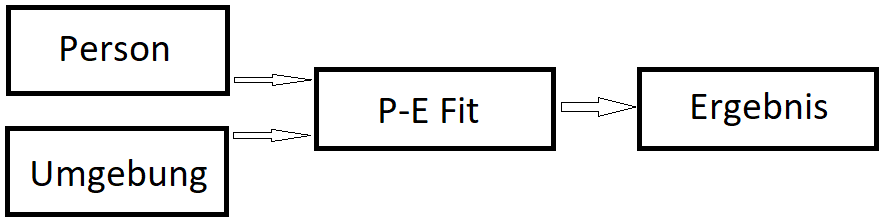
\includegraphics[width=1\textwidth]{gfx/P-E Fit.png}
	\caption{Hier eine Beschreibung einfügen und nochmal schön machen}
	\label{fig:personEnvironmentFit:einfuehrung:abb1}
\end{figure}
\\
In der Literatur wird unter dem P-E Fit meist kein Zustand, sondern ein andauernder Prozess verstanden.

- Vergleichbare Konstrukte mit vergleichbaren Dimensionen --> Wie verrechnen? --> Supplementary/Complementary

\section{Supplementary und Complementary Fit}
\label{ch:personEnvironmentFit:SupCompFit}
\newpage
https://www.sciencedirect.com/science/article/pii/S0001879115300129 \\
- Ähnlichkeit oder Kongruenz wird als Fit bezeichnet. Führt zu Outcome. Wie diese berechnet wird --> Supplementary oder Complementary

- Nadler und Tushman 1980 \\
- Rynes und Cable 2003 stellten fest, dass Bewerber das Unternehmen bevorzugen, in welchen sie am besten performen können \\
- Mortimer und Lorence 1979 stellten fest, dass die Mitgliedschaft in einer Organisation die Werte und Persönlichkeit einer Person formt \\
Prozess!!!


GRUNDLEGENDES
- \cite[S. 53]{edwards:2008}: Bedeutung des Begriffes "fit": In der Literatur werden verschiedene Begriffe Synonym für Fit verwendet, z.B. Match, Ähnlichkeit, Kongruenz zw. Person und Umgebung --> Das sind klare Begriffe, welche die Nähe von Person und Umgebung zueinander bezeichnen --> Das ist laut Edwards die richtige Konzeptualisierung für fit; Viele Autoren verwenden Begriffe ohne klare Bedeutung wie Harmonie, Kompatibilität, etc.; Fit wird auch als Interaktion oder wechselseitige Beziehung bezeichnet; Um die Bedeutung des Begriffes fit zu klären, sollten laut Edwards Begriffe verwendet werden, welche sich auf die Annäherung von P und E zu beziehen und weniger Metaphern verwenden \\
%- \cite[S. 2]{edwards:2008}: Den Grundstein für die P-E fit Forschung haben insbesondere Murrays (zwei Quellen) Need-Press-Modell und Lewins Feldtheorie (Zwei Quellen) gelegt --> Ausgehend von dieser Arbeit (meint wahrscheinlich Lewin) ist der P-E fit als ein Kernkonzept in Jobzufriedenheit, Job Stress, Berufswahl, Rekrutierung und Auswahl und Organisationskultur und Klima hervorgegangen (zu allem Quellen) --> Diese verschiedenen Strömungen haben hunderte Studien generiert, die in Zusammenfassungen (Quellen) und Meta-Analysen (Quellen) gereviewed wurden \\
- \cite[S. 3]{su:2015}: Alle P-E fit Theorien teilen die folgende Annahme: Menschen suchen und erstellen Umgebungen, die es ihnen erlauben, durch ihr Verhalten ihre Charaktereigenschaften zu manifestieren (z.B. suchen dominante Personen Leitungsfunktionen); Das Ausmaß, zu dem Menschen in ihre Arbeitsumgebungen passen (fit), hat signifikante Auswirkungen (z.B. Zufriedenheit, Performance, Stress, etc.) --> Umso besser der fit umso besser die Ergebnisse \\
- \cite[S. 3]{su:2015}: P-E fit ist ein wechselseitiger und andauernder Prozess, bei dem Leute ihre Umgebung formen und die Umgebung die Leute formt (Quelle) \\
- \cite[S. 1]{caplan:1987}: Ein einzigartiges Merkmal des Frameworks ist seine Operationalisierung: Bewertung von P und E  Komponenten entlang von vergleichbaren Dimensionen \\
- \cite[S. 4]{caplan:1987}: Wenn man darlegen kann, wie der P-E fit erreicht wurde, kann das Mitgliedern der Organisation helfen zu bestimmen, ob Selektion, Training, menschliche Faktoren oder andere Ansätze ihre gewollten Effekte erreicht haben\\
- \cite[S. 5]{caplan:1987}: Besondere Anforderung der PE fit Theorie: P und E müssen entlang vergleichbarer Dimensionen bewertet werden --> Beispiel: "Wie viele Bücher über technische Updates wird von dir erwartet, zu lesen?" (E-Demand) und "Wie viele Bücher über technische Updates liest du pro Woche?" (P - Ability) / Durch vergleichbare Mess-Skalen ist es möglich direkt die P-E Diskrepanz zwischen objektivem und subjektivem fit über über die objektive Messung von P und E zu bestimmen \\
%- \cite[S. 1]{edwards:1996}: P-E fit ist ein weit verbreitet in der Forschung zu organisationalem Verhalten / P-E fit verkörpert die Prämisse, dass Outcomes nicht separat von P un dE entstehen, sondern eher von der Beziehung zwischen beiden (Quellen)\\
%- \cite[S. 1]{edwards:2004}: Laut P-E fit Paradigma, entstehen Einstellungen und Verhalten aus der Kongruenz zwischen den Attributen von Person und Umgebung (Quellen) --> Persönliche Charakteristiken enthalten individuelle biologische oder psychologische Needs, Werte, Ziele, Fähigkeiten oder Persönlichkeiten; Charakteristiken der Umgebung beziehen sich auf intrinsische oder extrinsische Belohnungen, physikalische oder physiologische Demands, kulturelle Werte oder Bedingungen der Umgebung wie Hitze, Verfügbarkeit von Essen, etc. / In der Organisationsumgebung haben Forschungen das P-E fit Paradigma verwendet, um Outcomes vorherzusagen, die alle Phasen des Arbeitslebens umfassen (Dazu einige Beispiele mit Quellen) \\
- \cite[S. 1]{edwards:2008}: Person-environment fit ist ein zentrales Konzept in der Forschung des organisationalen Verhaltens / \cite[S. 2]{edwards:2008}: P-E fit hatte für Jahrzehnte eine zentrale Person in der Forschung zu organisationalem Verhalten --> P-E fit bezieht sich auf die Kongruenz, Übereinstimmung (Match) oder Ähnlichkeit zwischen Person und Umwelt (siehe dazu: \cite{edwards:1998}, \cite{muchinsky:1987})\\


PROZESS
- \cite[S. 3]{su:2015}: P-E fit ist ein wechselseitiger und andauernder Prozess, bei dem Leute ihre Umgebung formen und die Umgebung die Leute formt (Quelle)
- \cite[S. 2]{caplan:1987}: P-E fit Theorie wird als Methode zum Verstehen des Prozesses der Anpassung zwischen Mitgliedern einer Organisation und deren Arbeitsumgebung vorgeschlagen \\
- \cite[S. 4]{caplan:1987}: Der Anpassungsgrad wird in der PE-Fit-Theorie als der Betrag der Verbesserung des PE-Fits im Laufe der Zeit definiert --> Anpassungsprozess bezieht sich darauf, wie Verbesserung (oder Verschlechterung) erreicht wird --> Wie in Fig 1 dargestellt, gibt es verschiedene Punkte der Intervention --> Einer kann sich auf objektive P und E beziehen; Einer kann sich auf den Versuch der Veränderung von den subjektiven Gegenstücken beziehen --> Im Text: Anpassung von objektiven und subjektiven P und E, z.B. durch Selektion oder Training \\


P-O
- \cite[S. 2]{schneider:1995}: Chatman (Quellen) forschte zum P-O Framework zum Verstehen von individuellem Verhalten in Organisationen\\
- Tom 1971 zeigt, dass Menschen Umgebungen bevorzugen, die ähnliche Persönlichkeitsprofile wie sie haben \\


%- \cite[S. 2]{edwards:2008}: Spezifische Typen des P-E fit beziehen sich auf die Bedürfnisse der Person und die Belohnungen des Umfeldes (Quellen), die Fähigkeiten einer Person und die Anforderungen der Umgebung (Quellen) und die Ähnlichkeit zwischen Person und sozialem Umfeld, welches sich auf Individuen, Gruppen, Organisationen oder Berufe beziehen kann (Quellen) \\
%- \cite[S. 1]{edwards:1990}: P-E fit charakterisiert Stress als eine Diskrepanz zwischen korrespondierenden Charakteristiken einer Person und der Umgebung --> Diese Diskrepanz steht im Verdacht, schädliche psychologische, physiologische und verhaltensbedingte Outcomes zu erzeugen --> Diese könnten sogar in erhöhter Krankheit und Sterblichkeit münden \\
%- \cite[S. 1]{edwards:1990}: Das Framework bildet den Kern vieler aktueller Theorien des organisationalen Stresses  --> Solche Theorien wurden z.B. von \textcite{copingAndAdaption:1974}, \textcite{mechanismsOfJobStressAndStrain:1982} (Noch mehr Autoren) \\
%- \cite[S. 2]{edwards:1990}: P-E fit ist laut Eulberg et al. 1988 der meist zitierte Modell im Bereich des organisationalen Stresses --> Dieses Paper (von Edwards) konnte keine einzige Studie finden, die frei von Fallstricken war \\
- \cite[S. 3]{edwards:1990}: Konzept des P-E fit gibt es auch in anderen Bereichen der Forschung zu organisationalem Verhalten --> z.B. bei \textcite{locke:1969} --> Job Zufriedenheit kommt von der Wahrnehmung, dass ein Job wichtige Job-Werte erfüllt \\
%- \cite[S. 5f.]{edwards:2007}: (Quelle): PE fit wird auf unterschiedlichen Leveln unterschieden, auf denen der PE-fit ausgeführt wird / Person ist immer (ich würde sagen: meist oder überwiegend; gibt auch Ausnahmen siehe \cite[S. 6]{edwards:2007}) auf einem individuellen Level, aber E bezieht sich in der Forschung auf unterschiedlichen Level --> z.B. auf Personen in einer Umgebung; andere Individuen wie Führungskräfte; Mitarbeiter; Arbeitsgruppen; Abteilungen; Organisationen, etc. (zu allem zahlreiche Quellen) \\
%- \cite[S. 1]{edwards:2007}: Outcomes z.B. Berufswahl, Job-Zufriedenheit, Job-Performance, Wohlbefinden \\
- \cite[S. 1f.]{edwards:2007}: Die Forschung zum PE fit hat 3 grundlegende Annahmen: 1. Es wird generell angenomen, dass der PE fit zu positiven Outcomes führt (Quellen); 2. Es wird oft angenommen, dass die Auswirkungen des PE-Fits die selben über mehrere Personen- und Environments Konstruke sind (Quellen); 3. \cite[S. 2]{edwards:2007}: Effekte des PE fits sind die selben, unabhängig von den absoluten Levels von P und E oder der Richtung ihrer Differenz --> Quellen, die Ähnlichkeiten berechnen; Annahmen wurden diskutiert und in Frage gestellt, halten sie sich dennoch weitgehend in der PE Forschung \\ 

- \cite[S. 3]{edwards:2007}: PE fit wurde in verschiedenen Wegen konzeptualisiert --> Generell kann der PE fit als "die Kongruenz, Match, Ähnlichkeit oder Korrespondenz zwischen der Person und dem Umfeld" definiert werden\\
- \cite[S. 49]{edwards:2008}: Ein paar Quellen definieren P und E explizit (Quellen), die meisten Theorien geben keine expliziten Definitionen (Quellen) oder beschreiben P und E in generellen Begriffen, die einzelne Konstrukte zusammenfassen (Quellen) / Wenige Theorien sagen, dass dass die Effekte des PE fits davon abhängen wie die Umgebung von der Person wahrgenommen wird (Quellen von Locke und McGrath) und eine Theorie betrachtet objektive und subjektive P und E als getrennte Konstrukte (Caplan, French, Harrison) --> Diese Theorien sind laut Edwards aber Ausnahmen von der Regel \\
- \cite[S. 53]{edwards:2008}: PE-fit als Konstrukt: P-E fit ist eine Aussage über das Niveau von P und E relativ zueinander --> Wenn P und E auf dem selben Niveau sind (egal ob auf einem niedrigen, mittleren oder hohen), dann existiert der Definition nach ein P-E fit --> Ist das Level nicht gleich, existiert ein P-E misfit \\
- \cite[S. 4]{su:2015}: P-O fit z.B. bei Chatman 1989 und 1991 --> Definiert Kongruenz zw. persönlichen Werten eines Mitgliedes der Organisation und den Normen einer Organisation --> Persönliche und organisations-Werte werden beide durch ihren Inhalt und ihre Intensität relativ zu anderen Werten definiert --> Nach Chatman können Werte der Organisation auch in dem Grad beschrieben werden, zu welchem die Werte von den Mitgliedern der Organisation geteilt werden --> Wie bei ASA kann der PO-fit bei Chatman durch einen Selektionsprozess erreicht werden, bei dem die Organisation Menschen akzeptiert, deren Werte zu denen der Organisation passen / Außerdem formulierte Chatman einen Sozialisationsprozess, durch welchen die Organisation seine Mitglieder beeinflusst, deren persönliche Werte in Einklang mit den Werten der Organisation zu bringen / Outcomes des PO-fits inkludieren Änderungen von persönlichen und Organisationalen Werten in Richtung eines erhöhten P-O fits / Individuen, die einen höheren Fit mit ihrer Organisation erreichen, kann zu positiven Karriere-Outcomes führen, inkl. erhöhten Betriebszugehörigkeit, Zufriedenheit, Commitment, Kompetenz, etc. / Auch Chatman stellt fest, dass ein sehr hohes Level an fit zu ineffektivem Verhalten auf Seiten von Individuum und Organisation führen kann --> Äußert sich z.B. in reduzierter Innovation \\
%- \cite[S. 5]{su:2015}: Konzept des P-E fits wurde genutzt, um viele organisationale Probleme wie Rekrutierung, Auswahl, Staffing anzugehen und zu erklären wichtige Outcomes wie Commitment \\
%- \cite[S. 5]{su:2015}: Es gibt viele verschiedene Formen des Environments, bei dem der fit konstruiert wird, z.a. P-O fit, P-J fit, P-Group fit, P-Supervisor fit, P-Vocation \\
%- \cite[S. 5]{su:2015}: Welche Attribute wichtig sind, unterscheidet sich je nach untersuchtem Level \\
- \cite[S. 5]{su:2015}: Werbel und Gilliland 1999 erstellten einen multilevel Ansatz, welcher den Selektionsprozess in Bezug auf P-J, P-O und P-G abbildet; P-J ist definiert als die Kongruenz zwischen Demands des Jobs und Skills, Knowledge und Abiligies des Job Kandidaten und soll vorhersagen den Leistungsstand des Kandidaten, sein technisches Verständnis und die Arbeitsinnovation; P-O bezieht sich auf die Kompatibilität zwischen den Needs, Zielen und Values des Bewerbers mit den Normen, Werten und Belohnungssystemen der Organisation und sagt voraus das Verhalten, Commitment und Zurückhaltung; P-G fit stellt die Ähnlichkeit zwischen einer Person und den Mitgliedern einer Arbeitsgruppe in Bezug auf deren Werte, Ziele, Persönlichkeit, etc. fest --> sagt voraus Kooperation und Performance \\
- \cite[S. 11f.]{su:2015}: Bei Dawis and Lofquist 1976 und 1978 bezieht sich die Korrespondenz nicht auf einen statischen Zustand, sondern eher auf einen Prozess der "corresponsiveness", in welchem P und E gegenseitig aufeinander reagieren --> Änderungen am Fit treten auf, wenn sich bei P und E aufeinander anpassen, um einen besseren Fit zu erzielen --> Zu diesem Ergebnis kommt auch Roberts 2006, dieser erweiterte Schneiders ASA Framework zu ASTMA (Attraction, selection, transformation, maniplulation, attrition) bei P-O Transaktionen --> Hierbei besagt insbesondere Transformation, dass sich Menschen durch ihre Arbeitserfahrungen ändern können, so kann sich ihr objektiver oder wahrgenommener fit ändern; Manipulation bedeutet, dass nicht nur passiv die Demands von E erfüllen, sondern aktiv die Organisation ändern oder ihre eigene Arbeitserfahrung anpassen, um den fit zu maximieren \\
- \cite[S. 1f.]{carless:2005}: PE fit ist als genereller Term konzeptualisiert, unter welchen mehrere spezifische Notationen des fits fallen --> In der Rekrutieruns- und Selektionsdomäne: PJ fit, als match zwischen Individuum und den Anforderungen eines spezifischen Jobs; PO fit, dem zwischen Individuum und breiteren organisationalen Attributen --> Mehr Forschung gibt es zu PO fit \\
\cite[S. 2]{carless:2005}: Es ist wahrscheinlich, dass Arbeitssuchende die Bandbreite an Überlappung zwischen ihren Charakteristiken und denen des Jobs und der Organisation evaluieren (Breaugh 1992)
- \cite[S. 2]{carless:2005}: Kristof 1996 S. 4-5 definierte PO fit als "die Kompatibilität zwischen Menschen und Organisationen, die auftreten, wenn (a) mindestens eine Entität bietet was die andere benötigt oder b) sie ähnliche grundlegende Charakteristiken teilen oder c) beides" --> Ist die Unterscheidung zw. Supplementary und Complementary fit \\
- \cite[S. 2]{carless:2005}: PJ fit ist konzeptualisiert als Match zwischen individuellem Wissen, Skills und Abilities (KSA) und den Anforderungen des Jobs oder den Needs/Desires eines Individuums und was vom Job geboten wird (Quellen) \\
- \cite[S. 3]{carless:2005}: Studien von Cable und DeRue 2002 zeigten, dass PO fit Wahrnehmung war assoziiert mit organisationfokussierten Outcomes (z.B. Identifikation) und PJ fit Wahrnehmung war assoziiert mit Job- und Karriere-fokussierten Ergebnissen (z.B. Karrierezufriedenheit, Jobzufriedenheit und Berufs-Commitment) --> Ein Job-Angebot anzunehmen basiert auf beidem (Quellen) \\

%- \cite[S. 27]{edwards:1991}: Porters Need Satisfaction Fragebogen (PNSQ --> Porter 1962) --> oft verwendet bei algebraischer Distanz --> Enthält 13 Items, welche Job-Attribute nach Maslows Bedürfnispyramide beschreiben und zwei zusätzliche Items für Gehalt und Wissen
%- \cite[S. 8]{edwards:2008}: (Bezogen auf Lewin): Laut \textcite{schneider:2001} sollte die Formel eher interpretiert werden, dass Person und Umgebung additiv, interaktiv, proportional oder auf andere Weise miteinander verbunden sind, was nicht P-E fit bedeutet \\
- \cite[S. 8]{caplan:1987}: Der erste reale Test der PE fit Theorie unter Verwendung vergleichbarer Messungen von P und E erschien in Pervin 1967a und 1967b in einer Studie der Adaption unter Universitäts-Studenten --> Schlechter Fit zwischen Menge an Struktur im Bildungsansatz der Universität und dem Bedürfnis des Studenten nach Struktur wurde mit akademischer Unzufriedenheit und einem Studienabbruch aus nicht-akademischen Gründen assoziiert --> Seit Pervins Foschung sind viele Tests zur PE fit Theorie durchgeführt worden (zahlreiche Quellen) --> In diesen nachfolgenden Arbeiten ist mit wenigen Ausnahmen zu beobachten, dass einander entsprechend gemessene P und E signifikant zur erklärten Varianz beitrugen, die über die erklärte Varianz durch P oder E alleine hinausgeht \\

\section{Supplementary und Complementary fit}
\label{ch:personEnvironmentFit:supplementaryUndComplementary}
So stellten beispielsweise \textcite[S. 1ff.]{schneider:1995} fest, dass bei Bewerbern alleine der subjektive P-E fit darüber entscheidet, zu welchen Unternehmen sie sich angezogen fühlen und nach der Einstellung verbleiben. \\
- \cite[S. 1]{cable:1997}: Schneider 1987 stellt mit seinem ASA Modell fest, dass Perssonen sich von den Unternehmen angezogen fühlen, mit welchen sie eine hohe Ähnlichkeit aufweisen \\
- \cite[S. 4]{edwards:2008}: Der P-E fit bezieht sich auf eine Kongruenz, match oder Ähnlichkeit zwischen Person und Umgebung --> Diese generelle Definition wurde von \textcite{muchinsky:1987} in supplementary und complementary fit unterschieden / Laut \cite[S. 269]{muchinsky:1987} entsteht ein supplementary fit, wenn eine Person ähnlich zu anderen Individuen im Umfeld ist / Ein Complementary fit entsteht laut \cite[S. 271]{muchinsky:1987} wenn ein Individuum mit seinen Stärken Schwächen oder Bedürfnisse des Umfeldes ausgleicht und umgekehrt --> Der complementary fit wurde später nochmal unterschieden, ob die Bedürfnisse auf Seiten der Person oder des Umfeldes auftreten (Quellen) \\
- \cite[S. 1]{edwards:2004}: Laut \textcite{muchinsky:1987} gibt es zwei langjährige Traditionen in der PE fit-Forschung: Complementary fit und supplementary fit --> Complementary fit tritt auf, wenn P oder E Charakteristiken anbieten, die der andere benötigt --> Zitat \cite{muchinsky:1987}: "Die Schwächen oder Needs der Umgebung weren von den Stärken des Individuums ausgeglichen und umgekehrt"; Complementary fit kann bedeuten, dass ein Mitarbeiter ein Skillset besitzt, das die Organisation benötigt oder dass eine Organisation die Belohnungen bietet, die ein Individuum will / Supplementary fit existiert, wenn eine Person und eine Organisation ähnliche oder übereinstimmende Charakteristiken besitzen --> Typischerweise bei der Untersuchung von Werte-Kongruenz zwischen Mitarbeiter und Organisation (z.B. bei Kristof 1996) verwendet \\
- \cite[S. 1]{edwards:2004}: Supplementary und Complementary fit haben sich unabhängig voneinander entwickelt \\
- \cite[S. 2]{edwards:2004}: Innerhalb der supplementary Tradition Forschung ist die Wertekongruenz am prominentesten insbesondere im Feld des Organisationalen Verhaltens (Quellen) / Individuelle Werte ist das was sie glauben was wichtig ist --> Dies steuert ihre Entscheidungen und Verhalten; Vergleichsweise bieten organisationale Werte Normen, die spezifizieren wie die Ressourcen der Organisation zugewiesen werden sollten und wie die Mitglieder einer Organisation sich verhalten sollten / Value congruence bezieht sich auf die Ähnlichkeit zwischen den Werten des Individuums und dem kulturellen Wertesystem einer Organisation (Quellen) / Menschen fühlen sich angezogener und vertrauen anderen, die ihnen ähnlich sind (Quellen); Außerdem finden es Angestellte komfortabler in einer Organisation zu arbeiten, in der Dinge, die dem Individuum wichtig sind, auch anderen Angestellten wichtig sind; Führt zu besseren persönliche Beziehungen (Quellen); Werte einer Organisation; Werte-Inkongruenz führt zu kognitiver Dissonanz und Unzufriedenheit (Quelle) \\
- \cite[S. 2]{edwards:2004}: Es gibt einen Unterschied zwischen psychologischer Need Erfüllung und Wertekongruenz: Forschung bei der Need Erfüllung beschreibt Needs als gewünschte Menge eines Attributes (z.B. wie viel Autonomie ein Mitarbeiter will); Im Gegensatz dazu konzeptualisiert die Forschung der Wertekongruenz Values als Wichtigkeit eines Attributes (z.B. Wie wichtig Autonomie dem Individuum ist) --> Es wird also nciht die Content-Dimension von Needs und Values unterschieden, sondern die konzeptuelle Dimension entlang derer Needs und Values variieren (z.B. Menge vs. Wichtigkeit) --> z.B. Job-Zufriedenheit definiert das anderes, Edwards definiert es aber so \\
- \cite[S. 3]{edwards:2004}: Value-Kongruenz und Need-Fullfillment sind nicht unabhängig voneinander: Die Values einer Organisation beeinflussen die Typen von Belohnungen, die die Organisation supplied (Quelle) und die Werte einer Person beeinflussen ihre Desires (Quelle) \\
- \cite[S. 3]{edwards:2004}: Bei einem bestimmten Unternehmen anzufangen, ist ein konkreter, offener Ausdruck der Werte einer Person (Quellen) --> Das was der Organisation wichtig ist, zu der die Person gehört, sendet Signale an die Gesellschaft über das Selbst der Person und gibt Implikationen für die Selbst-Definition (Quellen) --> Wenn die Werte der Person inkongruent mit den Werten der Organisation sind, wird die Person kognitive Dissonanz und negatives Job-Verhalten zeigen; Außerdem ist Kommunikation und Freundschaft mit anderen Angestellten schwieriger, wenn sie keine gemeinsamen Values halten (Quelle)\\
- \cite[S. 3]{edwards:2004}: Value Kongruenz und Need-Erfüllung sind nicht unabhängig voneinander --> Die Values der Organisation bestimmen die Arten von Rewards, die die Organisation bietet (Quelle) und die Values einer Person bestimmen seine oder ihre Desires (Quelle) \\
- \cite[S. 3]{edwards:2007}: Schlüsselunterscheidung in PE fit Literatur ist zw. Supplementar und complementary fit (Quellen); Supplementary fit tritt auf, wenn die Person (Zitat von \textcite[S. 269]{muchinsky:1987}): "ergänzt, verschönert oder besitzt Charakteristiken, welche ähnlich zu anderen Individuen" sind; Auch betrachtet der supplementary fit den Vergleich zwischen einer Person und seinem sozialen Umfeld / \cite[S. 4]{edwards:2007}: Complementary fit existiert, wenn eine (Zitat \cite[S. 271]{muchinsky:1987}) "Schwäche oder Need des Umfeldes durch eine Stärke der Person ausgeglichen wird und umgekehrt" --> Complementary fit bezieht sich darauf, welche Erweiterung sich P und Egegenseitig bieten, was der andere will / Der Complementary fit kann weiter unterschieden werden, ob die Anforderungen von E oder P erhoben werden (Quellen) / Anforderungen des Umfelds beziehen sich auf Demands an die Person --> Der Grad, zu dem diese Anforderungen durch Wisen, Skills, Fähigkeiten und Ressourcen durch die Person erfüllt werden, steht für den DA fit (Quellen) / Requirements der Person spiegeln dessen Needs wieder, welche biologische Notwendigkeiten zum Überleben und psychologische Desires, Motive und Ziele \cite{copingAndAdaption:1974} \\
- \cite[S. 6]{edwards:2007}: Supplementary fit wird oft bei P-O fit genutzt \\
- \cite[S. 1]{edwards:2004}: Complementary und supplementary fit repräsentieren 2 unterschiedliche Traditionen innerhalb des P-E fit Paradigmas --> sind parallele aber separate Strömungen \\
- \cite[S. 1]{edwards:2007}: Zusätzlich zum DA und NS fit gibt es auch einen Fit zwischen den Werten der Person und denen der Organisation und deren Mitgliedern (Quellen) \\
- \cite[S. 4]{su:2015}: Schneider 1987 entwickelte das Attraction-Selection-Attrition (ASA) framework, welches in der Personalauswahl eines der meist gepriesenen PE-fit Theorien im organisationalen Kontext ist --> ASA erklärt den Prozess, nach dem Menschen angezogen, ausgewählt werden und entweder bleiben oder verlassen das Unternehmen --> Es wird genutzt, um wichtige Outcomes wie Karriere-Wahl, organisationales Commitment und Umsatz zu erklären; ASA definiert den PE fit als Grad der Ähnlichkeit zwischen Individuen und der Arbeitsumgebung --> Schneider argumentierte dass Menschen von Organisationen angezogen werden, die ihnen helfen ihre Ziele zu erfüllen; Ähnliche Menschen werden daher von ähnlichen Rahmenbedingungen von Unternehmen angezogen und unter diesen werden diejenigen ausgewählt, welche der Organisation helfen, ihre Ziele zu erreichen --> Nach dem Beitritt zu einer Organisation können Individuen ihren fit reevaluieren und diejenigen, die einen Mangel feststellenkönnten das Unternehmen verlassen / Dieser Prozess führt dazu, dass die Organisation vom Typus der Menschen darin definiert wird --> Das erhöht die Homogenität innerhalb der Organisation --> Das führt bei Angestellten zu einer höheren Zufriedenheit, Anpassung und Performance --> Schneider stellt aber auch fest, dass eine hohe Homogenität auf lange Sicht die Fähigkeit der Organisation zur Veränderung schwächen kann \\
- \cite[S. 6]{su:2015}: \textcite{muchinsky:1987} unterschieden zwei Typen von fits: supplementary und complementary / Supplementary: Fit basiert auf Ähnlichkeit / Complementary: Grad, zu dem die Charaktristiken einer Person die Charakteristiken der Umgebung komplettieren --> Schwächen oder Needs der Umgebung werde durch die Stärken des Individuums ausgeglichen und umgekehrt \\
- \cite{su:2015}: Aus DA-Fit entstehen positive organisationelle Outcomes wie Gruppen-Performance und organisationale Effizienz \ SV-fit beeinflusst primär die Zufriedenheit des Individuums mit der Umgebung --> Umso zufriedener, umso eher neigt das Individuum dazu, in der Organisation zu bleiben

\section{DA und NS Fit}
\label{ch:personEnvironmentFit:DAundNS}
- \cite[S. 3]{edwards:1996}: Values (bei SV) repräsentieren bewusste Desires, die von einer Person gehalten werden (Quellen) und umfasst somit Präferenzen, Interessen, Motive und Ziele (Quellen) / Supplies beziehen sich auf die Menge, Frequenz und Qualität der Attribute der Umgebung, die die Values der Person erfüllen können (Quelle) / Supplies können entweder objektiv oder subjektiv vermittelt werden (Quelle), nur subjektive Abweichungen von S zu V beeinflussen den Strain (Quellen) --> Deshalb ist der Kernprozess des S-V fits einen kognitiven Vergleich zwischen wahrgenommener und gewünschter Menge, Frequenz oder Qualität der Bedingungen oder Ereignisse wahrgenommen von der Person vorzunehmen \\
- \cite[S. 5]{edwards:1996}: DA-fit bezieht sich auf das Match zwischen Anforderungen von E und Fähigkeiten (Abilities) von P / Abilities enthalten Skills, Wissen, Zeit und Energie, welche P heranziehen kann, um die Demands von E zu erfüllen / Demands bezieehn sich auf quantitative und qualitative Anforderungen an die Person un dkönnen objektiv (z.B. Fließbandgeschwindigkeit, Länge des Arbeitstages) oder sozial konstruiert (z.B. Gruppennormen, Rollenerwartungen) sein --> In beiden Fällen können nur die Demands, die P wahrnimmt Stress auslösen (Quellen); \cite[S. 5f.]{edwards:1996}: Kernprozess der dem DA fit unterliegt ist der kognitive Vergleich zw. wahrgenommenen Anforderungen und den A der Person, um diese Anforderungen zu erfüllen \\
- \cite[S. 2]{edwards:2004}: Psychologische Needs werden mit Supplies von E vergleichen --> Diese beziehen sich auf extrinsische und intrinsische Ressourcen und Belohnungen (z.B. Geld, soziale Involviertheit, etc.) \\
- \cite[S. 2]{edwards:2004}: Need Fullfillment Literatur (Quellen) fokussiert (hier) die psychologischen Needs, welche sich eher auf die psychologischen Needs, die durch Lernen und Sozialisation erworben werden statt auf biologische Bedürfnisse (z.B. Essen) / Theorien der psychological Need Fullfillment --> Besagen, dass Menschen unzufrieden werden, wenn die Angebote der Umgebung kleiner sind als das was die Person verlangt (desires) --> Zufriedenheit nimmt zu, wenn Supplies sich zu Desires vergrößern --> Was passiert, wenn Supplies die Desires übersteigen, kommt auf die jeweiligen Needs an --> Kann unterschiedliche funktionale Formen annehmen (Quellen)\\

- \cite[S. 3]{caplan:1987}: Beim NS fit fragt sich der Angestellte "Was habe ich von diesem Job?" und der Arbeitgeber fragt sich "Was muss ich bieten, um den Angestellten zu behalten?" / Beim DA fit fragt der Angestellte "Was muss ich bieten, um den Job zu behalten?" und der Arbeitgeber fragt "Was erwarte ich vom Angestellten?" --> Es ist wichtig zwischen diesen beiden fit Typen zu unterscheiden, wenn man das Behalten und die Performance einer Person vorhersagen möchte --> Betrachtet man nur einen Typ des fits kann das wichtige Elemente des Austausch-Prozesses außen vor lassen --> Diese Elemente sind aber notwendig, um die Pflichten und Erwartungen zu verstehen, welche den pychologischen Vertrag zw. Arbeitgeber und -nehmer formen \\
- \cite[S. 4]{edwards:2008}: Der Grad, zu welchem die Bedürfnisse der Person durch intrinsische und extrinsische Belohnungen des Umfeldes belohnt werden, wird als "needs-supplies fit" bezeichnet (Quellen) / Der Grad zu welchem die Bedürfnisse des Umfeldes durch die Fähigkeiten der Person erfüllt werden, bezeichnet man als "Demands-Abilities fit" (Quellen) --> Anmerkung von mir: Es gibt also entweder einen NS-Fit einen DA-Fit oder einen supplementary fit \\
- Irgendwo in \textcite{choi:2004}: Je besser die Kongruenz, desto eher entsteht Kreativität \\
- \cite[S. 6]{edwards:2008}: Manche Studien identifizieren Grenzen, die Bedingungen etablieren, unter denen P-E fit-Beziehungen auftreten sollten --> Dies Bedingungen werden als Moderatoren bezeichnet, die die Form oder Stärke der P-E fit Beziehung beeifnlussen --> Beispiel: Der Effekt von D-A wird stärker, wenn das Nichterfüllen der Anforderungen wichtige Konsequenzen hat (Quellen) / Grenz-Bedingungen können sich aber auch auf Limitierungen beziehen, unter denen sich eine Theorie nicht anwenden lässt, z.B. wen die Outcomes des fits auf organisationalem Level beschränkt sind (Quellen) \\
- \cite[S. 2]{edwards:1990}: Umfassendste Behandlung des P-E fit Ansatzes (bzgl. Stress) wurde von \textcite{mechanismsOfJobStressAndStrain:1982} durchgeführt --> Behandlung enthält zwei verschiedene Versionen des P-E fits --> Eine Version fokussiert die Korrespondenz zwischen Angeboten der Umgebung (Supplies) und persönlichen Werten, Motiven, Zielen (Values) --> S-V fit / Die andere Version fokussierte die Korrespondenz zwischen Anforderungen (Demands) der Umgebung und persönlichen Fähigkeiten und Fertigkeiten (Abilities) --> D-A fit --> \textcite{mechanismsOfJobStressAndStrain:1982} stellen fest, dass sowohl P als auch E subjektiv und objektiv beschrieben werden können --> Objektive P und E beziehen sich auf die Variablen, welche unabhängig von der Wahrnehmung des Individuums existieren --> Subjektive P und E beziehen sich dagegen auf Variablen wie sie vom Individuum wahrgenommen werden --> Zentrale These von \textcite{mechanismsOfJobStressAndStrain:1982}: Gibt es einen Misfit bei subjektiven S-V oder D-A, dann entstehen daraus negative psychologische, physiologische und verhaltens-Outcomes, die kollektiv als "strain" bezeichnet werden \\
- \cite[S. 2]{edwards:1990}: \textcite{mechanismsOfJobStressAndStrain:1982} beziehen sich explizit auf den P-E fit, aber es gibt auch viele andere Studien, die den P-E fit implizit behandeln --> S-V fit ist implizit in \textcite{schuler:1980}s Konzeptualisierung von Stress --> Diese enthält eine dynamische Bedingung, welche das Individuum potentiell davon abhält das zu sein, haben oder tun was sie oder er will (Desires) / Auch das kybernetische Framework von \textcite{cummings:1979} gibt an, dass eine Diskrepanz zwischen dem bevorzugten Status des Individuums und dem aktuellen Status in strain resultiert \\
- \cite[S. 2f.]{edwards:1990}: Der D-A fit erscheint in McGraths Stressmodell (Quelle nicht gefunden) --> Besagt, dass Stress durch Anforderungen des Umfeldes entstehen, welche die Fähigkeiten und Ressourcen einer Person übersteigen \\
- \cite[S. 3]{edwards:1990}: \textcite{karasek:1979} sagt, dass strain auftritt, wenn hohe Anforderungen mit geringen Fähigkeiten zur Beeinflussung der Aufgaben kombiniert werden (z.B. geringe Entscheidungsfreiheit) \\
- \cite[S. 3]{edwards:1990}: Der S-V fit kommt auch in der Job Charakteristiken Theorie nach \textcite{hackmanOldham:1987} vor --> Besagt, dass Motivation und Zufriedenheit entstehen, wenn Individuen mit einem starken Bedürfnis nach persönlichem Wachstum mit bereichernden (enriched) Jobs kombiniert werden \\
- \cite[S. 3]{edwards:1990}: Der D-A fit unterliegt laut Schneider 1978 und Smith und Robertson 1989 (noch nicht nach Quellen recherchiert) dem am verbreitetsten Personalauswahl-Modell --> Job Anforderungen analysieren, benötigte Fähigkeiten definieren und Personen anstellen, die diese Fähigkeiten beherrschen (Anmerkung von mir: Genauso arbeiten heute auch die meisten Recommender Systeme) \\
- \cite[S. 3f.]{edwards:1990}: Es gibt zwei Versionen des P-E fits: S-V fit und D-A fit --> Werden manchmal gemeinsam unter der Rubrik P-E fit zusammengefasst, unterscheiden sich aber fundamental in ihren unterliegenden Prozessen und ihren assoziierten Outcomes --> \cite[S. 4]{edwards:1990}: Liegt an den zugrunde liegenden Komponenten --> Der S-V fit empfiehlt einen Prozess bei dem das Individuum aus seiner persönlichen Wertestruktur schöpft, um die Umgebung damit zu evaluieren / Beim D-A fit sammelt das Individuum dagegen seine Fähigkeiten und Fertigkeiten, um die Anforderungen der Umgebung zu erfüllen --> Prozesse sind getrennt voneinander \\
- \cite[S. 4]{edwards:1990}: Manchmal kann der D-A fit indirekt das Wohlbefinden beeinflussen, wenn das Erreichen der Anforderungen der Umgebung ein inhärenter Wert des Individuums ist (und dadurch ein S-V fit entsteht) oder wenn die Auflösung einer D-A Diskrepanz ein Instrument zur Erreichung eines S-V fits in einer verwandten Dimension ist (sagt \textcite{mechanismsOfJobStressAndStrain:1982}) \\
- \cite[S. 4]{edwards:1990}: Im Unterschied dazu zeigen Beweise, dass es unwahrscheinlich ist, dass der S-V fit die Performance beeinflusst (siehe: \textcite{greene:1972} und \textcite{schwabCummings:1970}) \\
- \cite[S. 4]{edwards:1990}: Ursprünglich waren S-V und D-A komplett unterschiedliche Versionen des P-E fits (siehe \textcite{copingAndAdaption:1974}, \textcite{mechanismsOfJobStressAndStrain:1982}, \textcite{harrison:1978}) --> Unterscheidungen in unterliegenden Prozessen und den assoziierten Outcomes --> Nachfolgende Studien haben diese Unterscheidungen minimiert oder manchmal sogar ganz übersehen --> Manche haben z.B. S-V und D-A als alternative Vorhersageelemente für die selben Outcomes gesehen, z.B. strain (\textcite{jobDemandsAndWorkerHealth:1975}, \textcite{mechanismsOfJobStressAndStrain:1982}) --> Deren Begründung (siehe \textcite[S. 31]{mechanismsOfJobStressAndStrain:1982}): Effekte S-V und D-A basieren auf dem Ausmaß, zu dem Motive befriedigt werden --> Edwards sagt, dass die Trennung aber wichtig ist, weil sonst fragwürdig ist, ob man z.B. D-A überhaupt braucht --> Auch viele andere Autoren betrachten S-V und D-A als austauschbar oder verwechseln sie sogar  --> Edwards ist der Ansicht, dass die Trennung zwischen D-A und S-V bei Untersuchungen erhalten bleiben muss --> Siehe hierzu auch \textcite{mechanismsOfJobStressAndStrain:1982} \\
- \cite[S. 5]{edwards:1990}: Generell: Beziehung zw. S-V und D-A und ihre Auswirkungen auf Wohlbefinden und Performance würden stärker erleuchtet werden, wenn beide Formen in einer Untersuchungsdomäne betrachtet werden (z.B. S-V und D-A fit bzgl. den selben Jobcharakteristiken) \textcite{caplan:1987} \\
- \cite[S. 2f.]{edwards:1991}: Es gibt zwei breite Klassen von korrespondierenden P und J Konstrukten / Erste Klasse betrachtet die Desires des Angestellten und die Supplies des Jobs, um die Desires zu erfüllen --> Dies ist zentral bei Theorien zur Job-Zufriedenheit, Job Stress, Berufswahl, Motivation, Zielsetzung (Quellen); Desires wurden unterschiedlich definiert, z.B. als psychologische Needs, Ziele, Interessen, Präferenzen (Quellen) --> Jede bezieht sich auf die Attraktivität verschiedener Job-Attribute für den Angestellten und können daher unter der allgemeinen Rubrik Desires (Wünsche) betrachtet werden; \cite[S. 3]{edwards:1991}: Job-Supplies reichen von generellen Beruflichen Charakteristiken zu spezifischen organisationalen and Job-Attributen wie Gehalt, Teilhabe an der Entscheidungsfindung, Rollenklarheit, etc. (Quellen) / Zweite Klasse sich entsprechender Konstrukte bezieht sich auf die Anforderungen des Jobs und die Fähigkeiten des Angestellten --> Diese Theorien sind sehr verbreitet bzgl. Job-Stress, dienen aber auch als Prädikatoren von Performance und Bindung und Förderung (Quellen) --> \cite[S. 3f.]{edwards:1991}: Abilities werden üblicherweise durch die Eignung des Angestellten beschrieben (Quellen) oder Stellvertretern davon wie Erfahrung, Bildung (Quellen) --> \cite[S. 4]{edwards:1991}: Job-Demands enthalten quantitative und qualitative Arbeitslast, Anforderungen für adäquate Job-Performance (Quellen) \\
- \cite[S. 4]{edwards:1991}: Wichtig: entsprechende Messung von P und J Konstrukten --> P und J werden in den selben Inhaltsdimensionen ausgedrückt (Quellen) --> Beispiel: Gehalt messen, dasder Angestellte gerne hätte und Gehalt messen, das der Angestellte erhält --> Viele (Quellen) geben an, dass entsprechende Messungen wichtig sind, da sie die logische Basis zur Berechnung von fit-Indizes, insbesondere Differenz-Werten bieten \\
- \cite[S. 4]{edwards:1991}: (Bezieht sich auf Bild mit Pfeilen) / Weiteres Thema ist die Betrachtung der Effekte von P und J auf Outcomes / Eine verbreitete Form ist die Reduzierung von P und J auf einen Index typischerweise mit einem Differenzscore oder einer Differenz davo --> Verbreitet bei Job-Zufriedenheit (Quellen) und Job Stress (Quellen) --> (Nochmal weiterlesen, meiner Ansicht nach nicht so wichtig) \\
- \cite[S. 5]{edwards:1991}: Weiteres Thema sind die Outcomes der PJ fit Forschung --> Repräsentieren im wesentlichen die abhängige Variable \\
- \cite[S. 7]{edwards:1991}: Oft werden Erwartungen und Desires als austauschbar betrachtet (Quelle) --> Aber Erwartungen und Desires sind getrennte Konstrukte \\

\section{Verstärkung}
\label{ch:personEnvironmentFit:verstaerkung}
- \cite[S. 3]{su:2015}: Theory of Work Adjustment (Quelle): Betrachtet die "Anpassung" an die Erwartungen und Belohnungen der Arbeit --> Im TWA haben Angestellte und Arbeit eine wechselseitige Beziehung, die gemeinsam die Betriebszugehörigkeit beeinflussen; Arbeitsplätze verlangen von den Arbeitern bestimmte Abilities und Angestellte erwarten von ihren Arbeitsplätzen Suppply an "Reinforcers" (Rewards), welche bestimmte Needs erfüllen --> "Korrespondenz" (bzw. fit) zwischen Job und Job-Inhaber ist hoch, wenn Angestellter erfüllt oder übersteigt die benötigten Fähigkeiten für einen Job oder ein Job trifft oder übersteigt die Needs eines Angestellten --> Ein "satisfactory" Angestellter hat eine hohe Korrespondenz an Ähnlichkeiten und ein "satisfied" Angestellter hat eine hohe Korrespondenz bei Arbeitswerten und Needs --> \cite[S. 4]{su:2015}: Satisfaction und Satisfactoriness sagen die Job-Zugehörigkeit voraus; Unsatisfactory Angestellte werden gefeuert wohingege unsatisfied Angestellte das Unternehmen verlassen --> Theorie auch in aktueller Forschung aufgegriffen (2 Quellen von 2006 und 2011) \\
- \cite[S. 3]{edwards:2004}: Menschen akzeptieren und behalten Jobs hauptsächlich basierend auf den gebotenen Rewards für ihre Zeit-Investitionen und Talent (Quellen) \\
- \cite[S. 3]{edwards:1990}: Auch die Work Adjustment Theory von \textcite{workAdjustment:1964} zeigt, dass Zufriedenheit durch eine Korrespondenz zwischen jemandes Werten und verfügbaren Verstärkungsmustern auf der Arbeit entstehen \\

\section{Formen}
\label{ch:personEnvironmentFit:formen}
- \cite[S. 5]{edwards:1990}: Es gibt drei grundlegende Formen des P-E fits (bzgl. Stress): \cite[S. 5]{edwards:1990}: Erste Form fokussiert die Differenz zwischen vergleichbaren P und E Komponenten --> Umso größer die Differenz, desto größer der strain --> Wird z.B. verwendet von \textcite{mechanismsOfJobStressAndStrain:1982} und vielen anderen / \cite[S. 5]{edwards:1990}: Zweite Form fokussiert die Interaktion zwischen P und E --> Stress tritt auf, wenn Eigenschaften der Umgebung mit bestimmten persönlichen Eigenschaften kombiniert werden --> so z.B. vorgestellt von \textcite{cherringtonEngland:1980}, \textcite{lyons:1971}, \textcite{obrien:1980} und anderen --> Operationalisieren den P-E fit als Produkt übereinstimmender P und E Komponenten / \cite[S. 5]{edwards:1990}: Dritte Form betrachtet den Anteil/Verhältnis P, der von E erfüllt wird (manchmal wird auch die Differenz betrachtet) --> Strain nimmt zu, wenn die Proportion geringer wird --> So z.B. verwendet von \textcite{mechanismsOfJobStressAndStrain:1982} und anderen / \cite[S. 5]{edwards:1990}: Viele Autoren betrachten die verschiedenen Formen als austauschbar oder als vergleichbar /  \textcite{mechanismsOfJobStressAndStrain:1982} sagen, dass proportionale Form über Diskrepanz verwendet werden sollte, wenn Ratio-Skalen verfügbar sind, sagt aber auch, dass sich die Ergebnisse nicht nennenswert unterscheiden / \cite[S. 5]{edwards:1990}: Nähere Betrachtung der drei Formen zeigt, dass die drei Formen unterschiedliche theoretische Perspektiven auf die Beziehung zwischen P-E fit und strain haben / Die Diskrepanz-Form betrachtet P als einen Standard, gegen die E vergleichen wird --> Größere Abweichung wird dann mit mehr Stress assoziiert / Die Interaktive Form impliziert, dass die Stärke der Beziehung zwischen E und strain beeinflusst --> P ist also weniger ein Standard --> P modifiziert die Auswirkungen von E auf Stress / Proportionale From teilt Charakteristiken der beiden anderen Varianten --> P ist ein Standard gegen den E vergleichen wird und beefinlusst die Stärke der Beziehung zwischen E und strain / Im Gegensatz zur interaktiven Form impliziert die proportionale Form, dass der Effekt von P auf die Stärke der Beziehung zwischen E und strain fortlaufend kleiner wird, wenn P sich vergrößert \\
- \cite[S. 5]{edwards:1990}: Obwohl die Unterscheidungen eher theoretisch sind, zeigen sie auch wichtige methodische Implikationen --> Liegt daran, dass die drei Formen fundamental unterschiedliche funktionale Beziehungen zwischen P, E und strain zeigen --> Können gut als Oberflächen in einem 3D Raum betrachtet werden --> \cite[S. 7]{edwards:1990}: Obwohl die drei Formen des fits alle fundamental unterschiedlich sind, gibt es in der Literatur einige mathematische Transformationen, die diese Unterscheidungen undurchsichtig machen oder ganz entfernen --> Beispiel an einem Autor: Wollte die Diskrepanz durch die squared Differenz zwischen P und E zur Vorhersage von Stress bestimmen --> Diese Berechnung entspricht jedoch der interaktiven Form / Erkenntnis: Die drei Formen sind mathematisch und theoretisch verschieden --> Man muss sich überlegen welche Hypothese man zum Einfluss P und E auf Stress aufstellt und dann die drei Formen nicht als austauschbar betrachten --> Sonst entstehen statistische Tests, die nicht die ursprüngliche Hypothese prüfen --> Form muss mit den theoretischen Annahmen übereinstimmen \\

\newpage
\section{Historische Entwicklung}
\label{ch:personEnvironmentFit:historisches}
Die Wurzeln des Person-Environment Frameworks reichen zurück bis ins erste Jahrzehnt des 20. Jahrhunderts \cite[S. 1]{su:2015}. Zum damaligen Zeitpunkt beschäftigten sich Wissenschaftler und Psychologen in zahlreichen Ländern der westlichen Welt intensiv mit dem Thema der Personalauswahl \cite[S. 1]{salgado:2001}. Ein Hauptanliegen der Forscher war es, individuelle Unterschiede zwischen den Menschen anzuerkennen und bei der Berufswahl zu berücksichtigen \cite[S. 2ff.]{stern:1900}. Deren Ansichten zu Folge würde die gesamte Gesellschaft effizienter arbeiten, wenn Menschen eine zu ihren wissenschaftlich ermittelten Fähigkeiten passende Tätigkeit aufnehmen würden \cite[S.2]{kevles:1968}\cite[S. 3]{parsons:1909}. Im Zuge dieser Entwicklungen konzipierte der Bostoner Professor Frank Parsons eine Vorgehensweise zur Berufsfindung, welche im Jahr 1909 vorgestellt wurde \cite[S. 1]{su:2015}. \textcite[S. 5ff.]{parsons:1909} erkannte schon zum damaligen Zeitpunkt, dass das Gleichgewicht von eigenen Fähigkeiten und Anforderungen des Berufsumfeldes eine wichtige Ursache für Effizienz, Produktqualität und Bezahlung waren. Aus diesem Grund empfahl er jungen Menschen vor der Berufswahl zunächst ihre eigenen Fähigkeiten, die Anforderungen verschiedener Arbeitsplätze und die Beziehung zwischen beiden Seiten zu verstehen. Erst wenn eine Person diese Punkte unter Beaufsichtigung eines Berufsberaters und durch Verwendung verschiedener wissenschaftlicher Tests erfüllt, könne sie sich für einen passenden Beruf entscheiden. Heute gilt Parsons aufgrund dieser Gedanken als "Gründungsvater der Berufsberatung" \cite[S. 3]{porfeli:2009} und als erster Vorläufer des Person-Environment Frameworks \cite[S. 2]{edwards:2008}.\\
Zum damaligen Zeitpunkt begegnete die Bevölkerung psychologischen Tests zunächst mit Skepsis \cite[S. 2]{kevles:1968}. Das änderte sich im Jahr 1917 mit dem Eintritt der Vereinigten Staaten in den Ersten Weltkrieg. Das U.S. Militär stand vor der Herausforderung, innerhalb kürzester Zeit Millionen Männer in die verschiedenen spezialisierten Rollen des technisierten Krieges einzuordnen. Zu diesem Anlass setzten Wissenschaftler erstmals im großen Stil psychologische Tests zur Zuweisung von Personen zu passenden Militärpositionen ein \cite[S. 2ff.]{kevles:1968}. \\
Nach dem Ersten Weltkrieg entstanden insbesondere in den 1930er-Jahren durch die Arbeiten von Lewin und Murray weitere bedeutende Entwicklungen für die Entstehung des Person-Environment Frameworks \cite[S. 1]{edwards:1990}. \textcite[S. 11f.]{lewin:1936} stellte fest, dass das Verhalten eines Menschen nicht wie bis dahin angenommen nur durch das Individuum selbst, sondern durch das Zusammenspiel von Person und Umgebung zu erklären ist. Aufbauend auf diesen Erkenntnissen erarbeitete \textcite[S. 38ff.]{murray:1938} sein Need-Press-Modell. Der Wissenschaftler ging davon aus, dass jeder Mensch im Laufe seines Lebens verschiedene Bedürfnisse (Needs) unterschiedlich stark ausprägt. Diese treffen in verschiedenen Umgebungen auf diverse Reize. Murray stellte fest, dass manche Reize mit bestimmten Bedürfnissen kompatibel sind. Trifft ein passendes Bedürfnis-Reiz-Paar aufeinander, entsteht Druck (Press). Personen nehmen diesen als schädliche oder nützliche Situation wahr und zeigen eine entsprechende Reaktion. Dieses Zusammenspiel von Bedürfnissen einer Person und Reizen der Umgebung entspricht der späteren Vorstellung des Need-Supply fits im Person-Environment Framework \cite[S. 8]{edwards:2008}. \\
Die Erkenntnisse von Kurt Lewin und Henry Murray gelten als wichtiger Grundstein für die Arbeiten verschiedener Forschungsgruppen rund um John R. P. French, Jr. \cite[S. 5]{caplan:1993}. Der Psychologe stellte im Jahr 1963 an der Universität in Michigan ein groß angelegtes Forschungsprogramm vor. Dieses machte es sich zum Ziel, die Auswirkungen des sozialen Umfeldes in Industrie-Unternehmen auf die Gesundheit der Mitarbeiter zu untersuchen. Zu diesem Zweck arbeiteten Experten verschiedener Fachrichtungen eng zusammen \cite[S. 1ff.]{french:1963}. Aus dieser Kollaboration entstand die erste formale Definition des Person-Environment Frameworks, welche im Jahr 1974 von \textcite{copingAndAdaption:1974} vorgestellt wurde. In dieser unterschieden die Forscher ausgehend von vorherigen Erkenntnissen, dass nicht nur objektive Beobachtungen, sondern auch subjektive Wahrnehmungen des Mitarbeiters bei der Bestimmung des Fits bedeutsam sind \cite[S. 4f.]{caplan:1993}\cite[S. 1ff.]{french:1966}. \\
% Aus diesem Grund empfahl er (Murray), Reize und entsprechende Bedürfnisse mittels einander entsprechender Dimensionen zu messen. 

\section{Subjektive Wahrnehmung des P-E Fits}
\label{ch:personEnvironmentFit:subjektivObjektiv}
Bei der ersten Präsentation des Person-Environment Frameworks untersuchten \textcite{copingAndAdaption:1974} die Auswirkungen des Zusammenspiels von Individuum und Arbeitsumgebung auf die mentale Belastung des Mitarbeiters. Wie in Abbildung \ref{fig:personEnvironmentFit:subjektivObjektiv:abb1} dargestellt, gingen die Wissenschaftler davon aus, dass von Person und Umgebung je eine objektiv messbare und eine vom Mitarbeiter subjektiv wahrgenommene Version existieren. \\
\begin{figure}[h]
	\centering
	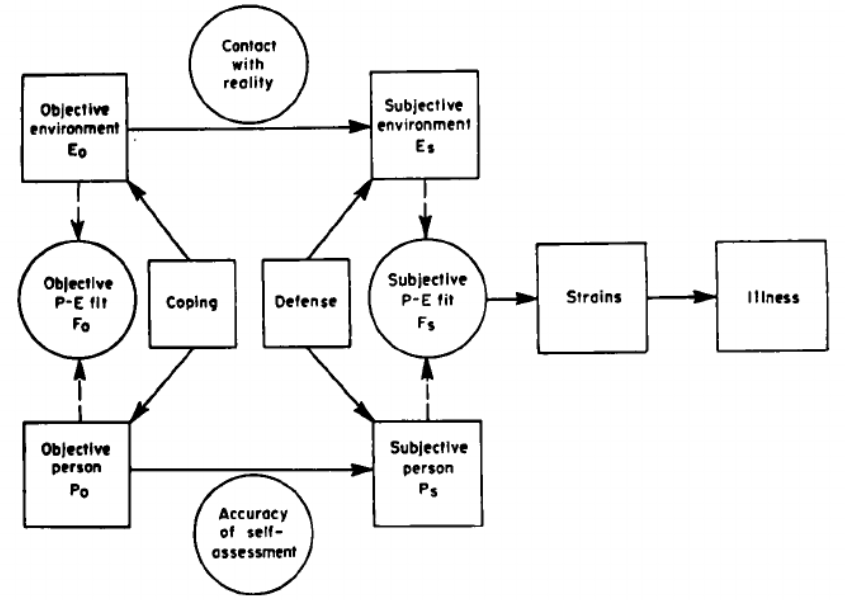
\includegraphics[width=1\textwidth]{gfx/subjektivObjektivPEFit.png}
	\caption{Hier eine Beschreibung einfügen \cite[S. 22]{edwards:2008}}
	\label{fig:personEnvironmentFit:subjektivObjektiv:abb1}
\end{figure}
\\
\textcite{copingAndAdaption:1974} betonten die Wichtigkeit, alle vier Subjekte anhand vergleichbarer Dimensionen zu messen. Dies betrachteten die Forscher als wichtige Grundlage, um aussagekräftige Ähnlichkeiten berechnen zu können. In ihren Untersuchungen bestimmten sie die in Abbildung \ref{fig:personEnvironmentFit:subjektivObjektiv:abb1} dargestellten Differenzwerte des objektiven \mbox{(F\textsubscript{O} = E\textsubscript{O} - P\textsubscript{O})} und des subjektiven \mbox{(F\textsubscript{S} = E\textsubscript{S} - P\textsubscript{S})} P-E Fits. Individuen streben den Wissenschaftlern zu Folge an, unerfüllte Anforderungen zu vermeiden. Dies gilt sowohl für unbefriedigte Wünsche der Person als auch überhöhte Ansprüche der Umgebung. Um solche Situationen zu vermeiden, existieren zwei Strategien. Ändert ein Mitarbeiter seine objektive Umgebung oder sein objektiv ermitteltes Selbst zur Verbesserung des objektiven P-E fits, sprechen \textcite{copingAndAdaption:1974} von Bewältigung (Coping). Ändert die Person ihre subjektive Wahrnehmung von Umgebung oder sich selbst zur Optimierung des subjektiven P-E fits, bezeichnen sie die Strategie als Verteidigung (Defense). Bei ihren Untersuchungen stellten die Forscher fest, dass der subjektive P-E Fit besonders bedeutsam für die Entstehung psychischer Belastungen und daraus resultierenden Krankheiten beim Mitarbeiter ist. Andere Werte wie der objektive P-E fit spielen dagegen nur eine untergeordnete Rolle. \\
Auch Publikationen anderer Forscher bestätigen die Einschätzung, dass der subjektive P-E fit aussagekräftiger für die Bestimmung von Ergebnissen ist, als der Objektive \cite[S. 3]{carless:2005}. Dementsprechend wird die subjektive Wahrnehmung des P-E Fits in der Literatur stärker fokussiert \cite[S. 8]{caplan:1987}\cite[S. 9]{caplan:1993}\cite[S. 16]{choi:2004}.\\
In einer auf den Erkenntnissen von \textcite{copingAndAdaption:1974} aufbauenden Arbeit kam \textcite{harrison:1978} sogar zu der Einschätzung, dass innerhalb des subjektiven P-E fits alleine der Needs-Supplies Fit Auswirkungen auf die mentale Gesundheit des Mitarbeiters hat. Ein Ungleichgewicht im Demands-Abilities Fit führe dagegen nur dann zu psychischer Belastung, wenn diese der Erfüllung des Needs-Supplies Fit schade. Als Beispiel für einen solchen Sachverhalt nennt \textcite{harrison:1978} eine performanceabhängige Gehalts-Auszahlung. Möchte ein Mitarbeiter die Bezahlung erhalten (Need), welche vom Arbeitgeber in Aussicht gestellt wird (Supply), hat aber nicht ausreichende Fähigkeiten (Abilities), um die dafür notwendigen Anforderungen (Demand) zu erfüllen, führe dies zu Unzufriedenheit. Der Grund ist jedoch nicht das unterschiedliche Niveau von Fähigkeiten und Anforderungen als solches, sondern die aus diesem Ungleichgewicht resultierende beeinträchtigte Bedürfniserfüllung des Mitarbeiters. Zu einer ähnlichen Einschätzung kommen auch \textcite[S. 1ff.]{lazarus:1978}. Diese untersuchten den durch das Zusammenwirken von Person und Umgebung entstehenden Stress. Dieser entwickelt sich den Einschätzungen der Wissenschaftler zu Folge nur, wenn das Individuum durch die Nichterfüllung von Anforderungen negative Konsequenzen befürchtet. Dabei kann es sich entweder um schädliche Folgen für die Gesundheit oder die Nichterfüllung innerer Werte und Ziele handeln. \\
Zusammenfassend lässt sich feststellen, dass zu wenig erfüllte Anforderungen in der Literatur meist eindeutig als Auslöser für negative Auswirkungen interpretiert werden \cite[S. 5]{schuler:1980}. Zu sehr erfüllte Anforderungen können dagegen unterschiedliche Folgen für Individuum und Organisation haben.

\section{Auswirkungen erhöhter Angebote}
\label{ch:personEnvironmentFit:auswirkungenErhoehterAngebote}
In der Literatur stellen \textcite{mechanismsOfJobStressAndStrain:1982} drei mögliche Auswirkungen vor, welche gegenüber den Anforderungen überhöhte Angebote annehmen können. Diese vertieften die Autoren auch in nachfolgenden Arbeiten \cite[S. 5f.]{caplan:1987}\cite{harrison:1978}(Harrison 1985). Die möglichen Auswirkungen erhöhter Angebote der Umgebung (Supplies) gegenüber den Bedürfnissen des Mitarbeiters (Needs) sind in Abbildung \ref{fig:personEnvironmentFit:auswirkungenErhoehterAngebote:abb1} dargestellt. \\
% Auch in Coping und Adaption?
\begin{figure}[h]
	\centering
	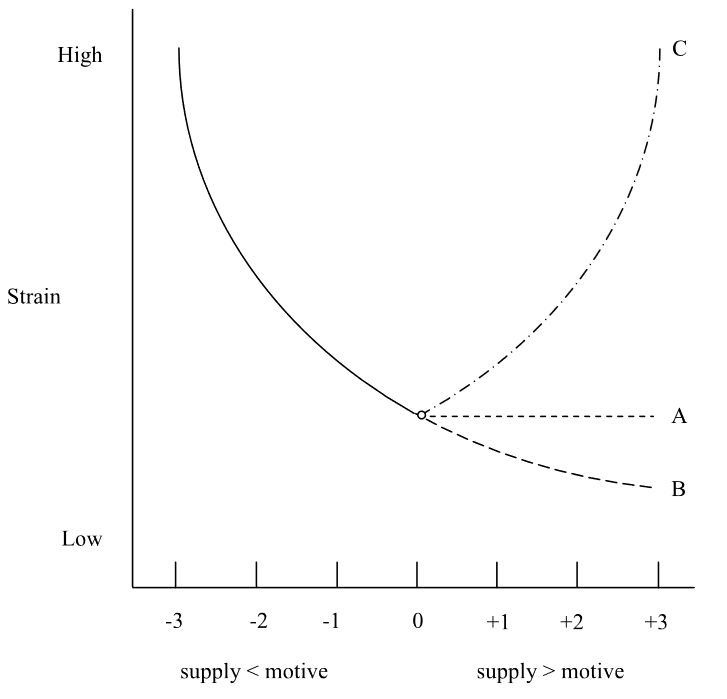
\includegraphics[width=1\textwidth]{gfx/ueberschuss_supply_motive.png}
	\caption{Hier eine Beschreibung einfügen (Beschriftung A und B tauschen) \cite[S. 23]{edwards:2008}}
	\label{fig:personEnvironmentFit:auswirkungenErhoehterAngebote:abb1}
\end{figure}
\\
An der durchgezogenen Linie in Abbildung \ref{fig:personEnvironmentFit:auswirkungenErhoehterAngebote:abb1} ist zu erkennen, dass je weniger die Bedürfnisse (Needs) einer Person erfüllt werden, die mentale Belastung (Strain) des Individuums stärker zunimmt (Quelle). Übersteigen die Angebote der Umgebung (Supply) dagegen die Bedürfnisse der Person, mündet dies in einer der drei gepunkteten Linien A, B oder C. Kurve A stellt eine asymptotische Beziehung der Überangebote zur mentalen Belastung dar. Sie tritt ein, wenn eine Person die Übererfüllung eines Bedürfnisses entweder für einen späteren Zeitpunkt aufsparen oder für die Befriedigung verwandter Motive investieren kann \cite[S. 5f.]{caplan:1987}. Dieser Sachverhalt ist beispielsweise erfüllt, wenn einer Person mehr Gehalt zusteht, als diese für die Zahlung ihrer Lebenskosten benötigt. Das überschüssige Geld könnte diese entweder für die Zahlung von Lebenshaltungskosten in den Folgemonaten aufsparen oder zusätzlich ihr mögliches Bedürfnis nach Luxusgütern befriedigen. Linie B ist U-förmig und tritt ein, wenn eine Übererfüllung eines Bedürfnisses entweder die Befriedigung dieses oder eines verwandten Motivs hemmt \cite[S. 5]{caplan:1987}. \textcite{harrison:1978} nennt hierfür das Bedürfnis einer Person nach sozialem Austausch als Beispiel, welches durch Übererfüllung deren Wunsch nach Privatsphäre verletzt. Kurve C stellt eine monotone Beziehung zur mentalen Belastung dar und tritt ein, wenn weder die Bedingungen von Kurve A noch von Kurve B zutreffen. Eine Übererfüllung dieses Bedürfnisses hat also weder positive noch negative Folgen für die Person. Ein Beispiel für eine solche Beziehung wäre ein Überangebot an vergünstigten Heißgetränken am Arbeitsplatz. Der Mitarbeiter kann die zusätzlichen Angebote nicht für einen späteren Zeitpunkt aufsparen, da diese in der Zwischenzeit abkühlen würden. Auch muss er nicht mehr trinken als er möchte, sodass keine negativen Auswirkungen auf dessen Wohlbefinden entstehen. \\
\textcite{harrison:1978} geht davon aus, dass ähnliche Beziehungen von Angeboten zu mentaler Belastung auch zu erwarten sind, wenn das Fähigkeitsniveau des Mitarbeiters (Abilities) die Anforderungen der Umgebung (Demands) übertreffen. Die entsprechend in Abbildung \ref{fig:personEnvironmentFit:auswirkungenErhoehterAngebote:abb2} dargestellten Beziehungen gelten wie in Kapitel \ref{ch:personEnvironmentFit:subjektivObjektiv} beschrieben jedoch nur, wenn das Erfüllen der Anforderungen der Umgebung zur Befriedigung innerer Werte und Ziele des Individuums beiträgt. \\
\begin{figure}[h]
	\centering
	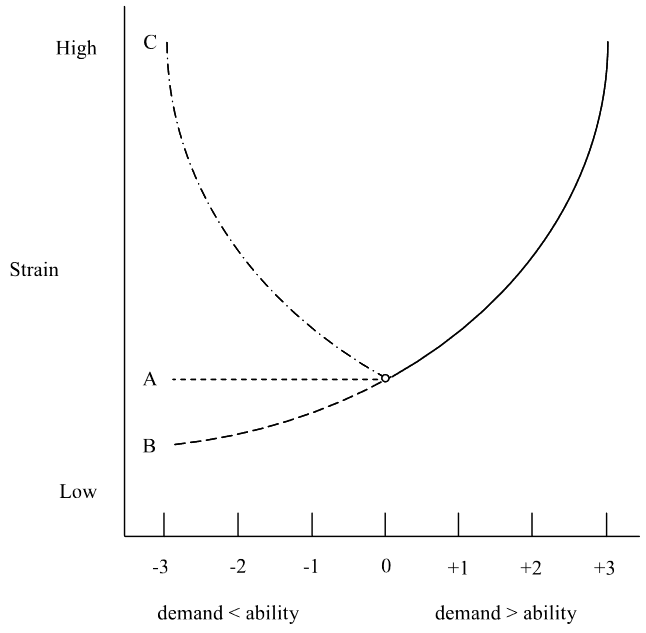
\includegraphics[width=1\textwidth]{gfx/ueberschuss_demand_abilities.png}
	\caption{Hier eine Beschreibung einfügen (Beschriftung A und B tauschen) \cite[S. 23]{edwards:2008}}
	\label{fig:personEnvironmentFit:auswirkungenErhoehterAngebote:abb2}
\end{figure}
\\
Zu ähnlichen Erkenntnissen wie \textcite{caplan:1987, copingAndAdaption:1974, harrison:1978, mechanismsOfJobStressAndStrain:1982} kommt auch \textcite{locke:1969}. Dieser betont, dass der Verlauf der Kurven in den Abbildungen zusätzlich stark von persönlichen Wichtigkeiten der Anforderungen bzw. Angebote ist. 
% Die historischen Bücher sprechen immer nur von "Männern" --> kann man daraus einfach "Menschen" machen?
% Gründungsvater ist ein englisches Zitat --> Wie zitieren?
% Wie umgehen mit den englischen Begriffen? z.B. fit, Need, Desire, etc.
\newpage
- \cite[S. 5]{caplan:1987}: Es gibt drei grundlegende Kurven, welche die Beziehung zw. PE fit der Angestellten und deren Levels von strain oder Kranksein beschreiben --> Dazu Bild im Text / Kurve A hat eine U-Form und repräsentiert die Bedingung, in welchem ein überschüssige Elemente einen Need bedrohen und ein Defizit an Elementen ein anderes Bedürfnis bedrohen kann --> bsp. Überschuss an Demand kann den Need eines Angestellten bedrohen, etwas zu erreichen und zu wenig Demand kann den Need eines Angestellten nach Stimulation bedrohen / \cite[S. 5f.]{caplan:1987}: Kurve B zeigt eine asymptotische Beziehung: Zeigt den Fall dass entweder ein Überschuss an E (Demands, Ressourcen) oder ein Überschuss an P (Needs, Abilities) das Kranksein erhöhen können --> Ein Defizit aber nicht --> Beispiel: Wenn eine P ein hohes Bedürnis nach Führung hat (Quelle) kann sie sich durch zu viele Möglichkeiten zur Entscheidungsteilhabe bedroht fühlen --> Reduzierung dieses Überschusses reduziert den Strain einer P bis zu einem Punkt, zu dem der Need erfüllt ist, nach diesem Punkt hat es nur noch wenig Strain-Reduzierende Effekte / \cite[S. 6]{caplan:1987}: Kurve C zeigt den Fall, in dem die absolute Menge einer PE fit Komponentente, relativ zu einer anderen, einen linearen Effekt auf Strain hat --> Beispiel: Je mehr Arbeit eine P relativ zur gewünschten Arbeitsmenge hat, desto mehr Strain entsteht / Es gibt auch noch weitere Kurven --> Bsp: Wenn es Intervalle gibt oder Tiefpunkt nicht exakt bei P=E liegt --> z.B. diskutiert bei Kahana 1978 oder Kulka 1979 \\
- \cite[S. 3]{edwards:1996}: Die meisten Theorien besagen, dass Strain zunimmt wenn S gegenüber V zu kurz kommt (Quellen), sind aber zweideutig bei einem Überschuss an S --> Harrison 1978 identifiziert 4 unabhängige Prozesse --> Erste zwei Prozesse geben an, dass ein Überschuss an S den Strain weiter reduziert. Erster wird als "Conservation" bezeichnet und tritt auf, wenn der Überschuss einbehalten werden kann, um den Fokuswert zu einem späteren Zeitpunkt zu befriedigen, z.B. angesammelte Urlaubstage oder überschüssiges Gehalt; 2. "Carryover": Überschuss von einem S hilft andere V zu erfüllen --> Tritt für V auf, die instrumentell verwandt sind, z.B. wenn ein Überschuss an Autonomie die Person dazu befähigt, gewünschte Veränderungen an der Arbeit vorzunehmen; Sowohl Conservation als auch Carryover zeigen eine monotone Beziehung zwischen S-V fit und Strain --> Strain nimmt weiter ab, wenn S V übersteigen / Die verbleibenden beiden Prozesse geben an, dass ein Überschuss an S den Strain erhöht: Erstes wird "depletion" genannt und tritt auf, wenn ein Überschuss an S die zukünftige Erfüllung von V auf der Fokusdimension verhindert --> z.B. Zu viel Unterstützung der Führungskraft zu einem bestimmten Zeitpunkt kann seine Unterstützung zu einem späteren Zeitpunkt ausschließen; 2. ist "Interference" --> \cite[S. 4]{edwards:1996}: Überschuss an S auf einer Dimension verhindert V-Erfüllung auf anderen Dimensionen --> z.B. Überschuss an Kontakt mit Mitarbeitern hindert das Verlangen nach Privatsphäre (Harrison 1978) --> Beide Prozesse zeigen eine gekrümmte Beziehung zw. Strain , sodass ein perfekter S-V fit optimal ist (und zu minimalem Strain führt) \\
- \cite[S. 6]{edwards:1996}: Die meisten Theorien besagen, dass Strain zunimmt wenn wahrgenommen wird, dass Demands zu hoch sind; Unterschiedliche Theorien was passiert, wenn Abilities zu hoch sind --> Ein Ansatz ist die Ansätze von Carryover, Conservation, etc. auch hier anzuwenden \\

- \cite[S. 9]{edwards:1996}: Es sind auch Sonderfälle möglich, z.B. wenn ein Überschuss an Demands den Value einer P erfüllt, sich selbst weiterzuentwickeln, dann kann der Strain trotzdem sinken \\
- \cite[S. 4]{edwards:1990}: Unterschiedliche Outcomes werden in verschiedenen Arbeiten diskutiert, z.B. Wenn Angebote der Umgebung von den individuellen Werten abweichen, entsteht Unzufriedenheit bei \textcite{locke:1969} / Im Gegensatz dazu: Übersteigen die Anforderungen der Umgebung die persönlichen Fähigkeiten, werden laut \textcite{theoryOfBehaviorInOrganizations:1980} Leistungseinbußen (Performanceeinbußen) wahrscheinlich \\
- \cite[S. 21]{edwards:2008}: Es gibt unterschiedliche Theorien wie es sich aber verhält, wenn die Supplies die Motive übersteigen --> Dann kann Strain zunehmen, abnehmen oder konstant bleiben --> Hängt davon ab, welche Auswirkungen die Übersteigung auf das Motiv oder andere Motive hat; Wenn das Überangebot nicht auf andere Motive angewendet werden kann oder für das Motiv nicht haltbar gemacht werden kann, dann sollte der NS-fit eine asymptotische Beziehung zum Strain haben (Kurve A); Wenn die übersteigenden Supplies zurückgehalten werden oder Motive anderer Dimensionen damit erfüllen können, sollte die monotone Beziehung von Kurve B entsteht --> Beispiel: Mehr Gehalt kann in Zukunft für Luxusgüter oder Dienstleistungen ausgegeben werden; Es entsteht eine U-Kurve, wen der NS fit andere Dimensionen oder dieselbe Dimension hemmt (Kurve C) \\
- \cite[S. 22f.]{edwards:2008}: Ein Ähnliches Verhalten stellen verschiedene (Quellen) auch beim demand-abilities fit fest --> (Aber nur, wenn DA misfit dazu führt, dass die Nichterfüllung der Anforderung den Erhalt von gewünschten Supplies hemmt)--> Wenn Demand größer als Abilities sind, entsteht Strain; Ist es umgekehrt, kommt es darauf an, wie die Kurve aussieht \\
- \cite[S. 21]{edwards:2008}: Weitere Arbeiten haben dieses Modell danach diskutiert (Quellen) --> Wie sich der Needs-Supply fit verhält, wird in mehren Arbeiten behandelt --> Alle sind sich einig, dass Strain zunimmt, wenn die Supplies des Environments die Needs der Person nicht erfüllen; Es gibt unterschiedliche Theorien wie es sich aber verhält, wenn die Supplies die Motive übersteigen --> Dann kann Strain zunehmen, abnehmen oder konstant bleiben --> Hängt davon ab, welche Auswirkungen die Übersteigung auf das Motiv oder andere Motive hat; Wenn das Überangebot nicht auf andere Motive angewendet werden kann oder für das Motiv nicht haltbar gemacht werden kann, dann sollte der NS-fit eine asymptotische Beziehung zum Strain haben (Kurve A); Wenn die übersteigenden Supplies zurückgehalten werden oder Motive anderer Dimensionen damit erfüllen können, sollte die monotone Beziehung von Kurve B entstehtn --> Beispiel: Mehr Gehalt kann in Zukunft für Luxusgüter oder Dienstleistungen ausgegeben werden; Es entsteht eine U-Kurve, wen der NS fit andere Dimensionen oder dieselbe Dimension hemmt (Kurve C) \\
- \cite[S. 22f.]{edwards:2008}: Ein Ähnliches Verhalten stellen verschiedene (Quellen) auch beim demand-abilities fit fest --> (Aber nur, wenn DA misfit dazu führt, dass die Nichterfüllung der Anforderung den Erhalt von gewünschten Supplies hemmt)--> Wenn Demand größer als Abilities sind, entsteht Strain; Ist es umgekehrt, kommt es darauf an, wie die Kurve aussieht \\
- \cite[S. 24]{edwards:2008}: Außerdem hat Harrison die Effekte des P-E fits auf den organisationalen Strain untersucht, welcher sich auf Probleme der Funktionsweise , welche die Produktivität und das Überleben der Organisation verhindern --> Organisationaler strain entsteht, wenn die Fähigkeiten der Angestellten unzureichend sind, um die Rollen-Anforderungen zu erfüllen / Harrison 1985 S. 42 stellt fest (Zitat), dass das erfüllen der Needs und Values fundamental für das weitere Funtionieren und existieren des Individuums genauso wie das erfüllen der Rollenanforderung fundamental für das funktionieren und existieren der Organisation ist --> In Sonderfällen kann aber auch ein N-S fit zu organisationalem Strain führen / Beziehung zw. D-A Misfit und organisationalem Strain kann laut Harrison 1985 wie in Figur 4.6 betrachtet werden --> Org. strain nimmt zu, wenn die Anforderungen die Abilities übersteigen, aber bleibt konstant, nimmt ab/zu wenn die Abilities die Demands übersteigen \\

\section{Wichtigkeiten}
\label{ch:personEnvironmentFit:wichtigkeiten}
- \cite[S. 23f.]{edwards:2008}: Harrison 1985 betrachtete, wie Wichtigkeit die Auswirkungen des P-E fits beeinflusst --> Schlägt vor (Harrison 1985, S. 38), wenn man einen P-E fit über mehrere Dimensionen macht könnte man die Wichtigkeit jeder Dimension in die Formel integrieren , die die Diskrepanz jeder P-E fit Dimension mit der Wichtigkeit dieser Dimension multipliziert \\
- \cite[S. 9]{edwards:1996}: Laut Caplan 1987 wurden verschiedene Variablen als potentielle Moderatoren des Effektes von SV fit und DA fit auf Strain --> Eine gemeinsame Variable bei SV und DA ist Wichtigkeit --> \cite[S. 10]{edwards:1996}: Es wird vermutet, dass Wichtigkeit die Effekte von SV und DA fit auf Strain intensiviert, sodass ein Misfit auf wichtigeren Dimensionen zu größerem Strain als ein Misfit auf weniger wichtigen Dimensionen führt (Quellen)\\
- \cite[S. 10]{edwards:1996}: Obwohl die Wichtigkeit die Beziehung zwischen SV und DA zu Strain moderieren, unterschiedet sich der unterliegende psychologische Prozess zwischen SV und DA fit --> Bei SV fit zeigt der moderierende Effekt der Wichtigkeit die Prämisse, dass ein Missfit ist schädlicher für die stark gehaltenen Values (Quellen); Beim DA-fit basiert die wichtigkeits-Moderation auf dem Grad zu welchem der Misfit zu wichtigen Konsequenzen führt, d.h. solche welche beinhalten substantielle Rewards oder Kosten für die Person (Quellen) --> P evaluiert, ob die Konsequenzen begehrenswert oder nicht begehrenswert sind --> Ähnlich dem Bewertungsprozess bei SV; Der DA misfit wird als wichtig angesehen, wenn er zu einem SV misfit auf anderen Dimensionen führt --> Diese Korrespondenz zw. SV und DA zeigt, dass ein DA misfit einen SV fit nicht nur verhindern kann wenn Abilities Demands übersteigen, sondern auch wenn Demands Abilities übersteigen \\
- \cite[S. 20f.]{edwards:2008}: Schon \textcite{copingAndAdaption:1974} sagten dass man Wichtigkeiten verwenden sollte. Sagten aber nicht wie.


\section{Perfekter Fit}
\label{ch:personEnvironmentFit:perfekterFit}
- \cite[S. 4]{edwards:2004}: Kristof 1996, S. 6 stellt fest: "Der optimale P-O fit ist erreicht, wenn jeder Need einer Entität ist erfüllt durch einen anderen und sie teilen dieselben grundlegenden Charakteristiken" \\
- \cite[S. 23]{edwards:2008}: Es gibt auch Erweiterungen des Frameworks, die Minima an anderen Punkten als dem P-E fit haben --> Caplan 1983 S. 39 sagt z.B. dass der meist emotional zufriedenstellenste Punkt so liegt, dass er eine kleine Herausforderung generiert. / Es gibt noch weitere Erweiterungen, z.B. wie Vergangenheit und Zukunft den Fit beeinflussen könnten \\
- \cite[S. 6]{caplan:1987}: Dass der Tiefpunkt nicht bei P=E liegt, wurde bei Kobasa\&Puccetti 1983 diskutiert)


\section{Skalen}
\label{ch:personEnvironmentFit:skalen}
- \cite[S. 14]{caplan:1987}: Es gibt bei Messungen von P und E die Bedenken, dass diese mit Elementen des anderen verunreinigt sind --> ist insbesondere Möglich, wenn Antwortskalen mit relativen Quantitäten arbeiten z.B. Arbeitsbelastung auf einer Skala von 1 (keine) bis 5 (eine Menge) eher als mit absoluten Quantitätn (z.B.  Anzahl Bücher) --> Relative Bewertung von E-Demands wie "sehr viel" kann sich auf "Im Vergleich zu gestern", "Im Vergleich zu anderen Angestellten", etc. beziehen --> Deshalb sollten keine relativen Antwortskalen verwendet werden  \\
- \cite[S. 5]{edwards:1993}: French et al 1982 haben Supplies und Preferences durch Itempaare gemessen --> Beispiel für Itempaar: "Wie viel Arbeitslast hast du?" und "Wie viel Arbeitslast würdest du gerne haben?" --> Antwortskalen reichten von "sehr wenig (1)" bis "sehr viel (5)" \\
- \cite[S. 5]{edwards:2008}: Dann können noch unterschiedliche Einheiten zur Konzeption von P und E verwendet werden --> Needs können z.B. über Einheiten oder Wichtigkeiten ausgedrückt werden --> Diese Unterscheidung hat wichtige Implikationen für die Theorien des N-S fits (Quellen) \\
- \cite[S. 8]{edwards:1990}: Messung der P und E Komponenten sollte vergleichbar sind --> Heißt: Sollten dieselbe theoretische Dimension haben --> \textcite{copingAndAdaption:1974} sagen, dass vergleichbare Messungen notwendig für Differenz-Berechnung sind --> Das ist laut \textcite{jobDemandsAndWorkerHealth:1975} die meistverwendete Prozedur in der P-E fit Forschung --> Differenzberechnungen werden meist verschiedenen Transformationen ausgesetzt, um den Punkt des 'Perfect Fit' zu bestimmen \textcite{jobDemandsAndWorkerHealth:1975} / Wenn diese Prozeduren genutzt werden, müssen die P und E Messungen nicht nur vergleichbar sein, sondern auch noch denselben Nullpunkt teilen --> sonst ist die Bestimmung des Punktes bedeutungslos \\
- \cite[S. 8]{edwards:1990}: Zweitens: Fragebögen, welche zur Messung der P und E Komponenten genutzt werden --> Sowohl bei SV als auch DA sind Fragebögen bzgl. E einfacher --> S-Fragebögen sollten fragen wie sehr das Attribut vorhanden ist, wohingegen D-Fragebögen sollten das Level (Höhe) der Demands erfragen, die mit einem betrachteten Attribut verbunden sind (vgl. \textcite{jobDemandsAndWorkerHealth:1975})/ Fragebögen zu P sind komplexer: Zu V gibt es zwei Möglichkeiten: Einmal zu erfragen, zu welchem Level die Attribute erfüllt sein sollen (\textcite{jobDemandsAndWorkerHealth:1975}) oder die Wichtigkeit der Attribute (\textcite{workAdjustment:1964}) --> Theoretische Diskussionen ergeben, dass der erste Ansatz eher für die Diskrepanz-Form und der zweite für die Interaktive Form geeignet ist (\textcite{copingAndAdaption:1974} und mehr Quellen) --> Es gibt auch Studien, die es anders bzgl. Diskrepanz machen (z.B. V durch Wichtigkeiten messen) oder manche Studien der interaktiven FOrm messen V in Desires --> Ergebnis: Ergebnisse dieser Studien lieern keine klare Interpretation über die grundlegenden Priznzipien des P-E fits / Für A veranschlagen Fragebögen oft ein Selbstassement der Fähigkeiten  oder indirekte Indikatoren der Fähigkeiten wie z.B. Bildung (\textcite{jobDemandsAndWorkerHealth:1975}) --> Vorteil des ersten Ansatzes: Man kann besser das Konstrukt messen, das einen tatsächlich interessiert, dafür ist der Ansatz anfällig für eine Antwortverzerrung durch soziale Erwünschtheit (social desirability response bias) --> Dieser Bias kann durch die zweite Methode vermieden werden, bietet aber eine weniger direkte Messung des Konstrukes, das einen interessiert --> Gibt keine klare Lösung, aber man sollte die Trade-Offs im Hinterkopf behalten \\
- \cite[S. 8f.]{edwards:1990}: Drittes Problem beachtet die Anzahl an fit-Dimensionen, die in die Studie eingebunden werden / Manche Studien (Quellen) verwenden nur eine Dimension / Sogar die systematischsten Untersuchungen zur Zeit von \cite{copingAndAdaption:1974} und \cite{mechanismsOfJobStressAndStrain:1982} enthalten nur acht Dimensionen des Fits / Wenn es nur wenige Dimensionen gibt, haben solche Studien zwei Nachteile --> 1. Wenn man annimmt, dass eine Inkongruenz über mehrere Dimensionen den strain stärker beeinflusst, vernachlässigen diese Studien notwendigerweise relevante Bestimmungsgrößen von Strain; 2. Diese Studien bieten nur limitierte Informationen über den P-E fit als generelles Konstrukt / Übergeordnete Ansätze involvieren umfassende Messungen von Person und Environment, um Indizes des fits zu bestimmen --> z.B. haben viele Studien zur Jobzufriedenheit den Work Values Inventory verwendet, um Indizes entlang von 15 Dimensionen zu bestimmen (Quellen genannt); Alternativ kann man auch Arbeitnehmer interviewn, um Job-relevante Aktivitäten und Konstrukt-korrespondierende Indizes des Fitszu erhalten --> Beide Prozeduren werden eine Einschätzung des fits bieten und sollten wenn möglich implementiert werden

\section{Berechnung}
\label{ch:personEnvironmentFit:berechnung}
- \cite[S. 1f.]{caplan:1993}: (French 1963) hielt eine Rede, in welcher er ein neues Programm für interdisziplinäre Forschung beschrieb, bekannt als Mental Health and Industry Program und heute als das Social Environment and Health Program am Institut für Sozialforschung (ISR) --> Dieses Programm generierte einige der ersten Tests der PE fit Theorie(Quellen) und einen großen Datensatz auf PE fit und Wohlbefinden von mehr als 2000 Angestellten und 23 Berufsgruppen --> Dieser diente auch für nachfolgende Tests als Ressource für Tests zur PE fit Theorie (z.B. bei \textcite{edwards:1993}) / French unterstrich in seiner Rede die Wichtigkeit der Messung von P und E entlang entsprechender Dimensionen / French beschrieb ein programmatisches Modell, dass besagt, dass Charakteristiken von P und E einen breiten Bereich von Antworten wie Verhalten, Stimmung, physische Gesundheit --> Von all diesen Reaktionen wurde angenommen, dass sie die physikalische und mentale Gesundheit beeinflussen --> Um die breiten Reaktionen zu untersuchen, stellte French Forscher verschiedener Disziplinen u.a. Epidemiologen, Physiker, Verhaltenspsychologen, etc. ein / \cite[S. 4]{caplan:1993}: Untersuchten die Verbindung zwischen Arbeitsbedingungen und Wohlbefinden / Datensatz stammt von Caplan,  Cobb,  French,  Harrison und Pinneau (1980) \\- \cite[S. 11]{caplan:1993}: Die meisten Arbeiten betrachten den PE fit eher als einen unabhängige Variable als einen Outcome (Gibt ein paar Ausnahmen; Hier mit Quellen) \\
- \cite[S. 15f.]{caplan:1993}: Edwards schlägt eine generelle Prozudur vor, die es erlaubt die Eignung von Bedingungen und Annahmen zu bestimmen --> Prozedur erlaubt die Beziehung zwischen outcome und Kongruenz auf drei Dimensionen (Bild-->zu sehen sind die Rohdaten von Caplan et al 1980) --> Dabei ist die abhängige Variable vertikal / \cite[S. 16]{caplan:1993}: Ansatz von Edwards: Statt einen Differenz-Wert zu berechnen, nimmt man die Regressionsgleichung der Modelle (z.B. von absoluter oder algebraischer Differenz) --> Dann bestimmt man Anteil der erklärten Varianz (??)\\
- \cite[S. 2]{edwards:1993}: Die P-E fit Theorie stellt drei hypothetische Beziehungen zwischen fit und strain vor --> Sind verkörpert in den five fit Messungen genutzt von (French) und (Caplan) / 1. Einfachste Messung genannt "fit" besteht aus der algebraischen Differenz zwischen E und P (E-P) --> Zeigt eine monotone Beziehung zum Strain --> Diese Beziehung wird erwartet, wenn z.B. Strain nicht nur abnimmt wenn S zu Motiven zunimmt sondern auch weiter abnimmt, wenn S übersteigt und kann auf andere Motive angewendet werden oder für spätere Verwendung zurückgehalten werden; Zwei Messungen, genannt "deficiency" (E-P für E <= P, 0 für E>P) und "excess" (E-P für E>=P, 0 für E<P) zur Darstellung von asymptotischen Beziehungen (Anmerkung für mich: Asymptotische Beziehung gab es auch bei \cite{edwards:1996}) zu Strain; Defiency repräsentiert eine negative Beziehung zu Strain nur wenn E ist kleiner als P --> Zunehmende S reduzieren den Strain bis zu einem Punkt an Zufriedenheit und haben nur noch wenig Effekt danach; Im Gegensatz dazu excess drückt eine positive Beziehung zum strain aus, nur wenn E größer ist als P --> Demands erhöhen Strain, wenn sie Abilities übersteigen, aber nciht wenn sie kleiner sind als Abilities / Zwei Messungen: "poor fit" (|E-P|) und die "squared difference" ((E-P)\^2) (hier genannt "fit squared") zeigen eine gekrümmte (curvilinear) Beziehung zum Strain --> Diese Beziehungen werden erwartet, wenn entweder übersteigen oder inadäquate S oder D sind schädlich, z.B. wenn zu viel Job-Komplexität zu einer Überlastung aber zu wenig zu Langeweile führt / Anm: Bilder zu allen Beziehungen vorhanden \\
- \cite[S. 2]{edwards:1993}: Es gibt viele Probleme an den 5 Messungen von Caplan und French (Quellen) --> Liegt an der Verwendung von Differenz-Berechnungen --> Es folgt Kritik dazu --> Probelme mit den fit Messungen können durch andere von Edwards beschriebenen Prozeduren überwunden werden --> Edwards führt in diesem Paper die Forschungen von French et al 1982 erneut aus und wendet seine empfohlenen Berechnungen darauf an --> \cite[S. 19]{edwards:1993}: Ergebnisse: 1. fit Messungen, die E und P in einen Wert zusammenrechnen sollten zugunsten von Polyomialgleichungen, welche E und P und geeignete Terme höherer Ordnung enthalten, aufgegeben werden (Quellen) / Edwards Studie demonstrierte, dass fit Messungen zu mehrdeutigen Ergebnissen führen, die separaten Beziehungen von E und P mit strain durcheinander bringen, einen sehr restriktiven Satz von Beschränkungen auferlegen, die selten unterstützt werden und reduzieren die inhärente dreidimensionale Beziehung zwischen E, P und strain auf zwei Dimensionen / \cite[S. 20]{edwards:1993}: Edwards (Quelle) Prozedur vermied diese Probleme und zeigte in den meisten Fällen, dass die Beziehung zwischen E, P und strain konnte nicht adäquat von den fit Messungen von French et al 1982 repräsentiert werden --> Grund: Diese Prozedur nutze Gleichungen, welche Fit-Messungen subsummieren, dies eliminierte die Notwendigkeit für diese Messungen und erlaubte darüber hinaus die Mesung von einer breiteren Rand von Oberflächen bezogen auf E und P zu strain --> Weitere Punkte (nachlesen) \\
- \cite[S. 2]{edwards:1990}: Sinn seines Papers: Viele Studien, die P-E fit bezüglich Stress untersuchen, sind mit ernsten theoretischen und methodischen Problemen geplagt, welche die Aussagekraft der Ergebnisse schmälern \\
- \cite[S. 3]{edwards:1990}: Dieses Paper fokussiert auf Probleme, die bei anderen Papern bzgl. Stress aufgetreten sind --> lässt sich aber auch auf andere Bereiche übertragen \\
- \cite[S. 7]{edwards:1990}: Es gibt zwei wichtige methodische Probleme in den P-E fit Studien bzgl. Stress: Erste bezieht sich auf die Messung er P und E Komponenten; Zweite betrachtet die Analyse der Beziehung zw. P E und strain \\
- \cite[S. 9]{edwards:1990}: Hier treten die größten Probleme auf / Die meisten Arbeiten bei der Diskrepanz-Form operationalisieren den Fit als algebraische Distanz (oder einer Transformation davon) zwischen vergleichbaren P und E Komponenten --> Ansatz erscheint intuitiv, die Verwendung von Differenz-Werten wurde aber stark kritisiert (einige Quellen) --> Ein Differenz-Score ist eine einfache Linearkombination seiner Komponenten --> \\
DAS NOCHMAL ANSEHEN MIT LÖSUNGSVORSCHLÄGEN \\
- \cite[S. 55]{edwards:2008}: Laut Edwards 1994 ist es das wahrscheinlich größte Problem Differenz-Werte und Profil-Ähnlichkeits-Indizes zu verwenden, um den P-E fit als eine einzige Variable auszudrücken --> Die Verwendung solcher Variablen wird oft auf theoretische Überlegungen zurückgeführt, z.B. könnte eine Theorie vorhersagen, dass der PE fit positiv mit einem Ergebnis zusammenhängt und als Reaktion wird ein Forscher Messungen von P und E zu einem Differnzwert zusammenfassung, um den P-E fit zu repräsentieren und den Wert mit der Messung eines OUtcomes korrelieren --> \cite[S. 56]{edwards:2008}: Geht nicht weiter darauf ein wurde in anderen (Quellen) schon behandelt --> Edwards macht sich eher Sorgen, dass die Berufung auf die Theorie, um die Verwendung von Differenzwerten und Profilähnlichkeitsindizes zu rechtfertigen, fehlgeleitet ist, da dies voraussetzt, dass die Theorie korrekt ist und sie von einer Überprüfung abschirmt --> Beispiel: Eine Theorie besagt, dass die absolute Differenz zwischen NS zu Zufriedenheit führt. Dann sollte nicht die Korrelation zwischen der absoluten Differenz zw. NS mit Zufriedenheit geprüft werden, sondern man sollte die Funktionsform testen, welche die absolute Differenz darstellen soll --> Diese Funktionsform sollte als zu empirisch zu testende Hypothese betrachtet werden und nicht als Annahme, die den Daten aufgezwungen wird --> ??? \\
- \cite[S. 7]{su:2015}: Verwendung von fit-Indizes ist wegen der Einfachheit des Kongruenzwertesn sehr beliebt in der Karriere-Entwicklungsforschung --> Kritisiert von Edwards --> Alternativer Ansatz von Edwards (1994, 2002): Nutzung von polynominaler Regression --> Basiert auf der Prämisse, dass P und E Messungen verschiedene Konstrukte sind und dass die funktionale Form sollte eher empirisch getestet werden als ein fit-Index angenommen zu werden; Laut Edwards sind die Gleichungen generalisierte Formen des fit-Indexes ohne ungewollte Annahmen über die Koeffizienten der Komponenten; Mit diesem Ansatz hat Edwards den Datensatz von French, Caplan und Harrison (1982) erneut analysiert und zeigte, dass er den Anteil erklärter Varianz mehr als verdoppeln konnte \\
- In \textcite{edwards:1991} werden sehr viele Methoden zur Verrechnung genannt \\

\section{Content von P und E Dimensionen}
\label{ch:notizen:contentVonPundEDimensionen}
- \cite[S. 6]{edwards:2007}: Dimensionen können auf einem Kontinuum von Generell bis speziell reichen --> Edwards schlägt drei Punkte vor: Global-, Domäne-, Facettenlevel der P und E Dimensionen / Beim globalen Level werden den Ähnlichkeiten als Ganzes ohne Bezug auf andere Vergleichsdimensionen miteinander verglichen --> beim Supplementary Fit genutzt --> z.B. um P und E oder P und andere P zu vergleichen (Quellen) / \cite[S. 7]{edwards:2007}: Domain-Level  isoliert breite Bereiche, aber unterscheidet keine Dimensionen innerhalb des Bereichs --> z.B. Werte, Persönlichkeit (Quellen) / Beim Facetten-Level wird die Ähnlichkeit spezifischer Dimensionen inerhalb breiter Bereiche verglichen, z.B. wenn man die demographische Ähnlichkeit nach Alter, Geschlecht, Rasse und Erziehung bestimmen will (Quellen) --> Gutes Bild dazu auf S. 10 \\
- \cite[S. 7]{edwards:2007}: Inhalt der P und E Dimensionen müssen vergleichbar sein (Quellen) --> Hat 2 Features: 1. Nominale Gleichheit: P und E werden mit denselben Begriffen beschrieben (sowohl bei SV als auch DA); 2. Skalengleichheit: Heißt, dass P und E mit derselben Metrik bewertet werden \cite{copingAndAdaption:1974} --> Wird erreicht, wenn dieselbe Antwortskala für P und E und unterschiedliche item stems (?) zur Unterscheidung von P und E verwendet werden --> Dieser Ansatz wird von Porters Need Satisfaction Questionaire (Quelle) vorgestellt --> Dort steht "Wie viel ist es jetzt" und "Wie viel sollte es sein"

\section{Job Zufriedenheit}
\label{ch:notizen:jobZufriedenheit}
- \cite[S. 9]{edwards:2008}: Theorien der Job-Zufriedenheit basieren auf der Prämisse, dass Job-Zufriedenheit aus dem Vergleich zwischen was ein Job bietet und was ein Angestellter benötigt, will oder verlangt vom Job (Quellen) --> Dieser Vergleich korrespondiert mit dem N-S fit in der P-E fit Literatur \\
- \cite[S. 10]{edwards:2008}: Katzell (Quelle) entwickelte ein theoretisches Modell, um die Beziehung zwischen Diskrepanzen in spezifischen Job-Facetten, Zufriedenheit mit Job-Facetten und insgesamter Job-Zufriedenheit zu erklären --> Katzell definierte Job Zufriedenheit als einen "Affekt oder Grundton", der mit einem Job assoziiert wird, der "aus der Interaktion zwischen Arbeitnehmern und ihren Job-Ereignissen entstehen: Arbeitnehmer besitzen Werte oder Bedürfnisse und der Job ist mehr oder weniger ein Instrument Erfüllung zu bieten oder Verstärken" --> Katzell bezeichnete Job Zufriedenheit als Beeinflussung vom Vergleich von den Werten des Angestellten und dem was der Job bietet / Katzell definiert Werte als "Größenordnung eines Reizes, die ein höheres Maß an Befriedigung hervorruft als diejenige, die von anderen Größen dieser Art von Reizen hervorgerufen wird" --> Das impliziert, dass die Zufriedenheit abnimmt, wenn die Stimuli in beide Richtungen von Werten abweichen. Katzell stellt dazu fest dass, "das Ausmaß zu dem ein Stimulus eine affektive Reaktion hervorruft, die weniger als maximal angenehm ist, ist direkt proportional zur absoluten Diskrepanz zwischen der Größe des Stimulus und seinem entsprechenden Wert und umgekehrt proportional zum Wert" --> wtf --> egal, steht sowieso sehr in der Kritik \\
- \cite[S. 12]{edwards:2008}: Locke entwickelte einer der einflussreichsten Diskrepanz-Theorien zur Job-Zufriedenheit / Locke definierte Job-Zufriedenheit als "den angenehmen emotionalen Zustand, der sich aus der Einschätzung ergibt dass die eigene Arbeit das Erreichen der eigenen beruflichen Werte ermöglicht oder erleichtert" (Quelle) --> Bewertungsprozess hat nach Locke 3 Elemente: 1. Die Wahrnehmung eines bestimmten Aspektes des Jobs; 2. Impliziten oder expliziten Wertestandard; 3. bewusstes oder unbewusstes Urteil über die Beziehung (z.B. Diskrepanz) zw. der Wahrnehmung und den Werten (Quelle) / Locke definiert Werte als etwas, das eine Person subjektiv "verlangt, will oder zu erreichen anstrebt" (Quelle) und fügte hinzu, dass Werte in Bezug auf Inhalt (was will die Person?) und Intensität (oder Wichtigkeit von dem gewollten) / Locke stellte zu den Werten die Needs in Kontrast, welche er als objektive Anforderungen für Gesundheit und Überleben beschrieb --> Locke sagte, dass Werte in Bezug zu Needs stehen, sodass "die ultimative biologische Funktion der Werte des Menschen es ist, seine Handlungen und Entscheidungen so zu lenken, dass sie seine Needs befriedigen" (Quelle) --> Locke vermutet, dass die Erfüllung der Werte zu Job-Zufriedenheit führt, vorausgesetzt, dass die Werte mit den Bedürfnissen vereinbar sind / \cite[S. 12f.]{edwards:2008}: Locke unterschied auch Werte von Erwartungen --> Sind Glaubenssätze über die Zukunft --> Locke ging davon aus, dass Diskrepanz zwischen Wahrnehmung und Erwartung zu einer Überraschung führt, welche befriedigend oder unbefriedigend sein kann, abhängig davon, ob das unerwartete Ereignis gewollt (desired) ist (z.B. Lottogewinn) oder ungewünscht ist (z.B. Gefeuert Werden) / \cite[S. 13]{edwards:2008}: Locke (Quelle) formalisierte seine Perspektive durch die folgende Formel:

\begin{equation}
	S = (V_c - P)V_i
	\label{fig:formel1}
\end{equation}

S steht für die Zufriedenheit (Satisfaction),  Vc für den Wert (Value Content), P für die wahrgenommene Menge und Vi für die Wichtigkeit des Wertes (Value Importance) / Locke sagt, dass entweder die absolute oder die algebraische Differenz abhängig vom Inhalt des Wertes verwendet werden muss / Zwei Beispiele mit Geld und Temperatur (Quellen) / \cite[S. 14]{edwards:2008}: Umso wichtiger der Wert, umso steiler die Kurve \\
- \cite[S. 14]{edwards:2008}: Möchte man mehrere Job-Faketten evaluieren, kann man diese addieren, um eine insgesamte Job-Zufriedenheit zu bestimmen / Einige nachfolgende Arbeiten bauen auf Locke auf (Quellen) / \cite[S. 15]{edwards:2008}: Locke erklärte, dass die Norm für Diskrepanztheorien nicht das ist was Leute erwarten oder objektiv brauchen, sondern was sie wertschätzen (value) / Locke führte auch aus, dass Menschen Werte nutzen, um ihren Job zu bewerten wie sie ihn wahrnehmen und nicht wie er aktuell ist (kann abweichen) / Lockes Modell hat aber auch einige Schwächen: 1. Zirkulär (ggf. nochmal ansehen); 2. Formel \ref{fig:formel1} ist inkonsistent mit den Beispielen von Locke inkl. den Bildern. Insbesondere (Vc-P) indiziert, dass die Zufriedenheit abnimmt, wenn die wahrgenommene Menge relativ zur gewünschten Menge steigt --> Das ist das Gegenteil des ersten Bildes; Interpretiert man (Vc-P) als absolute Differenz, dann hätte die Funktion eine V-Form, was das Gegenteil der Funktion in Abb 2 wäre. / Auch sagt locke nicht welche der beiden Berechnungsweisen für welche Job-Facetten zu nutzen sind. Er sagt nur, dass Abb 2 für die große Mehrheit der Job-Faketten genutzt werden sollte (z.B. Task-Schwierigkeit, Reisebereitschaft, etc.) (Quelle); Auch sagt er, dass die Wendepunkte und neutralen Punkte empirisch ermittelt werden müssen (Quelle) / Es kann auch andere Formen als in den beiden Abb geben / Locke selbst (Quelle) ermittelte basierend auf einer Literaturrecherche sieben Job-Facetten, die er als relevant für die Job-Zufriedenheit erachtete --> Legt dabei aber außer beim Gehalt keine Form des Graphen fest / Auch sagt Lockes Theorie wenig über Grenzbedingungen aus

\section{Job Stress}
\label{ch:notizen:jobStress}

\subsection{McGrath}
\label{ch:notizen:jobStress:mcgrath}
- \cite[S. 16]{edwards:2008}: Konzept des P-E fit ist weit verbreitet in den Theorien des Job Stresses (Quellen); Manche Theorien fokussieren den N-S fit (Quellen), andere den D-A fit (Quellen) und andere beide gleichzeitig (\cite{mechanismsOfJobStressAndStrain:1982}) \\
- \cite[S. 16]{edwards:2008}: McGraths Modell von Stress und Performance: McGrath (Quellen) fokussiert den D-A fit. Laut McGrath (Quelle) entsteht Stress durch ein Ungleichgewicht zwischen Anforderungen des Umfeldes und den entsprechenden Fähigkeiten --> Existiert nicht objektiv, sondern wie es von der Person wahrgenommen wird; Um Stress wahrzunehmen muss er Person das Ungleichgewicht bewusst sein / Stress kann sowohl bei einer Über- als auch einer Unterbelastung entstehen / Stress tritt nur auf, wenn die Person glaubt, dass die Konsequenzen des nicht erreichens der Anforderungen wichtig sind / Stress ist ein D-A Misfit, der zunimmt umso größer die Abweichung ist / McGrath stellte die folgende Formel auf (Quelle):

\begin{equation}
	ES = C(|D-A|)
	\label{fig:formel2}
\end{equation}

- \cite[S. 16]{edwards:2008}: ES ist der erfahrene Stress (experienced stress); C sind die wahrgenommenen Konsequenzen (Consequences); D sind die wahrgenommenen Anforderungen (Demands) und A sind die wahrgenommenen Fähigkeiten (Abilities) / \cite[S. 17]{edwards:2008}: In einer Studie operationalisierte McGrath Stress als eine physikalische Erregung und fand heraus, dass diese hoch war, wenn die Differenz zwischen Anforderungen und Fähigkeiten klein war (Quelle) --> McGrath interpretierte dieses Ergebnis als ein Manifestierung von Unsicherheit basierend auf der Annahme, dass die Unsicherheit eine Aufgabe zu erfüllen zunimmt, wenn die Anforderungen und Fähigkeiten nah beieinander sind --> Annahme: Erfolg wird wahrscheinlich, wenn Fähigkeiten die Anforderungen übersteigen und Verlust wird wahrscheinlich, wenn die Anforderungen die Fähigkeiten übersteigen --> Aus dieser Schlussfolgerung passte McGrath seine Formel an:

\begin{equation}
	ES = C(K-|D-A|)
	\label{fig:formel3}
\end{equation}

- \cite[S. 17]{edwards:2008}: K ist dabei eine Konstante --> Dadurch dass |D-A| von K abgezogen wird, zeigt die Gleichung, dass Stress (bzw. Erregung) zunimmt, wenn die Lücke zwischen D und A abnimmt \\
- \cite[S. 18]{edwards:2008}: Die Definition von Stress als Erregung wird in der Stress-Literatur diskutiert (Quellen)

\section{Berufliche Kongruenz}
\label{ch:notizen:beruflicheKongruenz}
- \cite[S. 25]{edwards:2008}: Der P-E fit ist zentral für Theorien der beruflichen Kongruenz, viele davon betrachten das Match zwischen Needs, Interessen und Fähigkeiten der Person und Verstärkern und Anforderungen (verschiedene Quellen) \\
- \cite[S. 26]{edwards:2008}: Wichtigster Forscher: Holland (Mehrere Quellen) \\
- \cite[S. 26]{edwards:2008}: Berufliche Kongruenz steht auch bei Theorien zu Arbeitsanpassung im Vordergrund

\subsection{Dawis und Lofquist}
\label{ch:notizen:beruflicheKongruenz:dawisUndLofquist}
- \cite[S. 28f.]{edwards:2008}: \textcite{workAdjustment:1964} legten den Grundstein für die Theorie des "Work adjustment" --> Konzeptualisierten die Person mit Abilities und Needs / Environment wurde beschrieben durc Ability-Requirements (benötigte Anforderungen für eine zufriedenstellende Arbeitsperformance) und ein Verstärkungssystem (Spezifikationen der verstärkten Werte von Klassen von Stimulusbedingungen) (In Klammern Zitate) --> Diese P E Konstrukte wurden in zwei Typen von Korrespondenz gemappt: Eine bezieht sich auf die Ähnlichkeiten zwischen Fähigkeiten der Person und den Fähigkeits-Anforderungen der Umgebung; Die andere betrachtet die Ähnlichkeit zwischen den Bedürfnissen einer Person und dem Verstärkungssystem der Umgebung --> \textcite{workAdjustment:1964} sagen, dass man die Begriffe zur Beschreibung von Abilities und Needs auch zur Beschreibung benötigter Fähigkeiten und verfügbaren Verstärkern genutzt werden sollten, sodass vergleichbare Dimensionen vorliegen --> Proximal Outcome der Korrespondenz ist dann Zufriedenheit (Definiton: "Die Evaluation des Individuums der Stimulus-Bedingungen der Arbeitsumgebung mit Bezug auf deren Effektivität bzgl. der Verstärkung seines Verhaltens") und Zufriedenstellung ("Evaluation des Arbeitsverhaltens in Bezug auf die Qualität und Quanität der Arbeitsperformance und/oder Performance-Outcomes (Produkte, Services)") / Zitate von \cite{workAdjustment:1964}: Zufriedenheit ist eine Funktion der Korrespondenz zwischen Verstärkungssystem der Arbeitsumgebung und den Needs des Individuums, vorausgesetzt dass die Fähigkeiten des Individuums mit den Fähigkeitsanforderungen der Arbeitsumgebung korrespondieren ... Zufriedenstellung ist eine Funktion der Korresondenz zwischen den Fähigkeiten des Individuums und den Fähigkeitsanforderungen der Arbeitsumgebung, vorausgesetzt, dass die Needs des Individuums mit dem Verstärkungssystem der Arbeitsumgebung korrespondieren" / Erkenntnis: Zufriedenstellung mäßigt die Effekte von Needs-Verstärkungssystem auf Zufriedenheit und genauso mäßigt Zufriedenheit die Effekte von Fähigkeiten-Fähigkeitsanforderungs-Korresponenz auf Zufriedenstellung --> "Work adjustment" ist definiert als kombinierte Levels von Zufriedenheit und Zufriedenstellung einer Person --> \cite{workAdjustment:1964} stellten auch fest, dass Zufriedenstellung und Zufriedenheit die Wahrscheinlichkeit beeinflussen, mit welcher eine Person in einer Arbeitsumgebung bleibt oder sie verlässt \\
- \cite[S. 29ff.]{edwards:2008}: Die Theorie wurde von Dawis et al. 1968 und Lofquist und Dawis 1969 grundlegend geändert und aktualisiert von Dawis und Lofquist 1984 \\
- \cite[S. 31]{edwards:2008}: Die letzte Version (Dawis und Lofquist 1984) definiert Fähigkeiten als empirisch abgeleitete Faktoren, die spezifische Fähigkeiten umfassen, die "wiederkehrende Reaktionssequenzen sind, die dazu neigen, durch Wiederholung modifiziert und verfeinert zu werden" (Zitat) / Analog dazu sind Values Faktoren, die spezifische Needs umfassen, die definiert sind als "Das Bedürfnis eines Individuums nach einem Verstärker auf einem bestimmten Niveau der Stärke" --> Stärke ist die Wichtigkeit eines Bedürfnisses --> Ich schließe aus dem Kontext: Je größer die Stärke, desto Häufiger muss die Reaktion des Verstärkers sein; Werte sind Wichtigkeitsdimensionen als Referenzdimensionen für die Beschreibung von Needs --> Needs sind Präferenzen für Verstärker ausgedrückt als relative Wichtigkeit für jeden Verstärker für das Individuum / Definition Korrespondenz: "Harmonische Beziehung zwischen Individuum und Umgebung, Eignung des Individuums für die Umwelt und der Umwelt für das Individuum, Übereinstimmung oder Einvernehmen zwischen Individuum und Umgebung sowie eine wechselseitige und ergänzende Beziehung zwischen Individuum und Umwelt" --> Es besteht also eine wechselseitige Beziehung zwischen Individuum und Umgebung / Definitionen für Zufriedenheit und Zufriedenstellung \\
- \cite[S. 32]{edwards:2008}: Kritik von Edwards an Dawis and Lofquist: Deren Theorie definiert Person und Umgebungs-Konstrukte auf eigene Art und Weise / \cite[S. 33]{edwards:2008}:  Auch sind Bedeutungen von Zufriedenheit und Zufriedenstellung unklar dargestellt

\section{Recruiting und Selektion}
\label{ch:notizen:rekcruitingUndSelektion}
- \cite[S. 33]{edwards:2008}: P-E fit ist fundamental, wenn Menschen mit Jobs in Unternehmen gematcht werden (Quellen) / Forschung in diesem Bereich identifiziert meist das notwendige Wissen, Fertigkeiten und Fähigkeiten für einen Job, misst diese Attribute bei möglichen Angestellten und untersuchen den Zusammenhang zwischen diesen Messungen und späterer Arbeitsleistung (Performance) --> Diese Forschung adressiert nicht direkt den Fit zwischen Person und Job, weil die persönlichen Attribute nicht berücksichtigt werden (Schneider, 2001) --> Edwards betrachtet nur Theorien, die explizit den P-E fit behandeln

\subsection{Wanous Matching Modell}
\label{ch:notizen:rekcruitingUndSelektion:wanous}
- \cite[S. 34f.]{edwards:2008}: Modell von Wanous ist eine Adaption der Work Adjustment Theorie von Lofquist und Dawis 1984 / Betrachtet SV- und den DA-fit / Auch hier gibt es Reinforcers / Abilities sind definiert als "was Menschen jetzt tun können oder potentiell in der Zukunft tun können werden" (Genauso auch die Anforderungen); Needs sind definiert als "grundlegendes Streben oder Verlangen"; Im Gegensatz dazu werden Verstärker und Anforderungen nicht explizit definiert / Laut Modell führt DA fit zu Job-Performance --> Zitat: Mismatch führt bei Fähigkeiten und Job-Anforderungen führt zu schlechter Performance; Match zwischen Bedürfnissen und Verstärkern führt zu Jobzufriedenheit und Organisationalem Commitment --> Definition Jobzufriedenheit: "Match zwischen Needs einer Person und erhaltener Verstärkung durch die erledigte Arbeit"; Definition Organisationales Commitment: "Dem Match zwischen Menschlichen Needs und den Verstärkungen, die man durch die das nicht-job Klima er Organisation erhält" / Johannes: Aus Modell ist abzulesen, dass Job-Performance zu einer Reaktion beim Unternehmen führt (Feuern, .., bleiben) und Job Zufriedenheit und Commmitment zu einer Reaktion beim Mitarbeiter (Gehen, bleiben) \\
- \cite[S. 35]{edwards:2008}: Später erstellte Wanous (1992) ein neues Modell getrennt von seinem alten Modell (Meiner Ansicht nach ändert sich da aber nicht viel)

\subsection{Breaughs Person-Job Congruence Model}
\label{ch:notizen:rekcruitingUndSelektion:breaugh}
- \cite[S. 36]{edwards:2008}: Braugh entwickelte ein Modell für einen Rekruting-Prozess der die person-job Kongruenz als zentrale Komponente unterstützt --> P-J Kongruenz definiert er als "Diskrepanz zwischen den Attributen, die ein e Organisation von einem potentiellen Angestellten verlangt und den Charakteristiken die eine Person bietet und die Diskrepanz zwischen dem was die Person von der Organisation will und den Anreizen, die der Arbeitgeber bietet" --> \cite[S. 37]{edwards:2008}: (Zitate) D-A fit führt zu einem zufriedenstellenden Level an Job-Performance und ein guter fit zwischen den Wünschen der Person und den Attributen der Job-Angebote führt zu einem Gefühl der Wertsteigerung, was wiederum zu Arbeitszufriedenheit führen wird" / Nachteil nach Edwards: Beschreibt keine Metrik, mit der Person und Job verglichen werden können --> Aber es gibt ein paar Beispiele / In einer Fußnote schreibt Breaugh, dass der P-J fit sich auf die Wahrnehmung der Kongruenz zw. DA und SV bezieht (das muss ich nochmal nachprüfen) / Modell bleibt auch wage bei der Form der Beziehung zwischen Kongruenz udn Outcomes --> In einer Fußnote stellt Breaugh fest, dass für manche Organisationalen Attribute ein Individuum weder zu viel noch zu wenig von einem Attribut sucht (z.B. Reisen). Bei anderen Attributen gitl, umso mehr die Organisation bietet (z.B. Bezahlung) desto besser wird die Person den fit bewerten --> Bestimmte Attribute werden aber nicht genannt

\subsection{Werbel and Gillilands Facet Model of Fit}
\label{ch:notizen:rekcruitingUndSelektion:werbel}
- \cite[S. 37]{edwards:2008}: Werbel und Gilliland stelleten ein Faketten-Modell des P-E fits vor, welches den Auswahlprozess in Bezug auf Person-Job fit, Person-Workgroup fit und Person-Organization fit bezieht / P-J fit ist definiert als (Zitat) Kongruenz zwischen Job-Anforderungen und den benötigten Skills, Wissen und Fähigkeiten eines Job-Kandidaten --> \cite[S. 38]{edwards:2008}: Laut 
Modell führt der P-J fit zu Leistung, technischem Verständnis und Arbeitsinnovationen / Person-Workgroup fit bezieht sich auf das (Zitat) Match zwischen dem Neuangestellten und der gesamten Arbeitsgruppe (z.B. Mitarbeiter und Führungskräfte) --> P-W fit wird sowohl durch einen supplementary als auch einen complementary fit bestimmt: Supplementary, da Werte, Ziele, Persönlichkeit übereinstimmen müssen und complementary, da die Gruppe heterogene Skills, Leistungen und Netzwerke mitbringen muss, sodass (Zitat) Performance-Schwächen eines Individuums durch die Performance-Stärken eines anderen Individuums ausgeglichen werden können / P-O fit enthält einen supplementary fit und einen needs-supply fit; Supplementary fit ist beschrieben als Kompatibilität zw. dem Wertesystem der Person und der Organisation; NS fit bezieht sich auf das Match (Zitat) zwischen den Bedürfnissen des Bewerbers und dem organisationalen Belohnungssystem --> Ergebnis des Fits sind Organizational Citizenship Behaviors (OCBs), organisationale Zufriedenheit, organisationales Commitment und Bewahrung / Die Outcomes aller drei fits sind mit insgesamter Performance und organisationaler Effektivität verbunden / Kommentare von Edwards: Modell ist dahingehend bemerkenswert, dass es drei Typen von P-E Fits betrachtet und kollektiv NS und DA und supplementary fit anspricht

\section{ToDo}
\label{ch:todo}
- Manche Arbeiten unterscheiden zwar explizit zwischen subjektiven und objektiven P und E --> Ausnahme von der Regel (Edwards) --> bei SV-fit ist subjektive Wahrnehmung üblich \\
- Am Anfang Edwards Definitionen für P, E, fit und P-E fit verwenden, danach einzelne Definitionen für die Konstrukte suchen \\
- Was ist organisationales Verhalten \\
- Gliederung: Wichtigkeiten und dann sagen, dass aber auch Autoren zum Ergebnis kommen, dass DA für Individuum vollkommen egal ist --> Reinforcers --> Obwohl diese Verstärker so wichtig sind, werden sie bei der Personal-Auswahl häufig vernachlässigt (nur DA) --> Diese fehlende Beachtung von SV spiegelt sich auch in der Implementierung von Empfehlungssystemen wieder --> Switch zu RS \\
- Merke ein Konstrukt ist z.B. Demand oder Supply \\
- Es ist nicht möglich, alle Varianten und Arbeiten zu behandeln, wie geht man damit um? \\
- Interessant: Supplies werden auch als "Verstärker" für Needs betrachtet \\
- Nochmal nach den Definitionen für DA und SV bei Edwards suchen \\
- Es gibt viele Arten von Fits (PO, PJ, PW, etc.) --> Klar machen, dass hier nur PJ fokussiert wird (PW siehe Werbel; PO siehe O-Klima bzw. Schneider bei Klima) \\
- Wichtigkeit spielt vor allem beim supplementary fit eine Rolle --> Dieser wird in dieser Arbeit eher ausgeklammert, weil ich mich auf P-J fokussiere und supplementary eher verwendet wird, um zu schauen ob eine Person zu anderen Personen oder überhaupt in eine Org passt. Dennoch spielen Wichtigkeiten auch in manchen Umsetzungen des complementary fit eine Rolle. --> Wichtigkeiten \\
- Wichtigkeiten beziehen sich bei SV auf die Werte bei DA auf die Konsequenzen --> Person ist es egal, ob sie Anforderungen erfüllt --> Neues Kapitel \\
- Eigentlich ist es mir als Person nur wichtig meine eigenen Werte zu erfüllen (SV) --> D.h. "Performance" ist nur ein Nebenergebnis der SV-Erfüllung \\
- Lazarus nochmal prüfen \\

\section{Fazit}
\label{ch:fazit}
- Ob man die Anforderungen der Stelle erfüllt, ist dem Mitarbeiter eigentlich egal. Ihn interessiert es nur, ob dadurch seine Werte verstärkt/erfüllt werden. Es wäre also interessant, herauszufinden, wieso ein Mitarbeiter z.B. mehr Python anwenden würde. Mehr Gehalt wegen Data Science? Neugier für neue Sprache? Kumpel arbeitet in dieser Abteilung? ... \\
- Eigentlich müsste der Prozess des Motivations-Herausfindens dem kompletten Einstellungsprozess vorgelagert sein. Bzw. sogar dem Studium \\
- Grenze: \textcite{cable:1997} stellten fest, dass das Bauchgefühl des Interviewers besser vorhersagen kann, ob eine P zur O passt. Wenn also ein Unternehmen so klein ist, dass der "Staffer" alle Berater persönlich kennt, kann er wahrscheinlich besser zuordnen als die KI \\
- Anmerkung von mir: Während \textcite{parsons:1909} 1909 also noch davon ausging, dass alles möglichst objektiv und wissenschaftlich korrekt gemessen werden muss, gehen Psychologen heute davon aus, dass primär die subjektive Wahrnehmung eine Hauptrolle spielt \\

\shorthandon{"}
\shorthandoff{"}
\chapter{Empfehlungssysteme}
\label{ch:empfehlungssysteme}
\section{Einführung}
\label{ch:empfehlungssysteme:einfuehrung}
Der Begriff des Empfehlungssystems ist im englischsprachigen Raum auch unter Bezeichnungen wie "Recommender System" \cite[S. 1]{lu:2015}, "Recommender Engine" \cite[S. 1]{panigrahi:2016} und "Recommendation System" \cite[S. 1]{ebesu:2018} verbreitet. Er wurde erstmals im Jahr 1997 von \textcite[S. 1]{resnick:1997} geprägt. Dass der Begriff gerade zu diesem Zeitpunkt entstand, ist auf die zur damaligen Zeit stark wachsende Internetnutzung und die damit verbundenen einfachen Möglichkeiten zur Sammlung und Auswertung großer Mengen an Nutzerdaten zurückzuführen \cite[S. xvii]{recommenderSystems:2016}.\\
Besonders bekannt für den Einsatz von Empfehlungssystemen sind große IT-Konzerne wie Amazon, Facebook, Google und Netflix \cite[S. 1]{zarzour:2018}. Diese Unternehmen nutzen Recommender Engines, um ihren Kunden personalisierte Vorschläge zu den Inhalten ihrer Plattformen anzuzeigen \cite[S. 2]{jeckmans:2013}. In vielen Fällen entfällt dabei für den Anwender vollständig die Notwendigkeit einer manuellen Suche \cite[S. 1]{comibingCareer:2013}.\\
Der Einsatz von Empfehlungssystemen wird in der Literatur kritisch diskutiert. Beispielsweise beobachteten \textcite[S. 17f.]{alfano:2020}, dass das Empfehlungssystem der Videostreaming-Plattform YouTube dazu tendiert, neuen Anwendern zur Verlängerung ihrer Nutzungszeit verschwörungstheoretische Inhalte auszuspielen. Eine Untersuchung von Forschern des sozialen Netzwerks Facebook kam zu dem Ergebnis, dass deren Recommender Engine Nutzern verstärkt Inhalte präsentiert, welche konform mit deren Ideologien sind \cite[S. 2]{bakshy:2015}. \textcite[S. 1ff.]{pariser:2012} prägte für diese Art der Personalisierung den Begriff der Filterblase.\\
Empfehlungssysteme haben aber auch einen bedeutenden Anteil am wirtschaftlichen Erfolg großer Internetplattformen. So führen beispielsweise \textcite[S. 6f.]{sharma:2015} etwa 30 Prozent des Internetverkehrs beim Online-Händler Amazon unmittelbar auf den Einsatz von Empfehlungssystemen zurück. \textcite[S. 5]{gomezuribe:2016} stellten bei einer Analyse der Streaming-Plattform Netflix fest, dass ca. 80 Prozent der Nutzungszeit auf Videos entfällt, welche Nutzern ohne vorherige Suche von einer Recommender Engine angezeigt wurden.\\
Um solche Vorschläge generieren zu können, suchen Empfehlungssysteme relevante Inhalte basierend auf den Präferenzen der Anwender aus \cite[S. 1]{das:2017}. Zu diesem Zweck müssen benötigte Nutzerdaten zunächst erhoben und in einer maschinell auswertbaren Struktur gespeichert werden.

\section{Zugrundeliegende Datenstruktur}
\label{ch:empfehlungssysteme:arbeitsweise}
Empfehlungssysteme können die Präferenzen ihrer Nutzer sowohl über explizite als auch implizite Rückmeldungen erfassen. Explizites Feedback erhalten Plattformen beispielsweise über abgegebene Produktbewertungen oder "Gefällt mir"-Angaben in sozialen Netzwerken. Um implizite Rückmeldungen auszuwerten, werden häufig Verhaltensweisen der Nutzer aufgezeichnet. Hierbei kann es sich beispielsweise um Suchverläufe oder die Wiedergabedauer von Videos handeln \cite[S. 3]{pu:2012}.\\
Das gesammelte Feedback überführen Analysten in die Struktur von Matrizen \cite[S. 11f.]{recommenderSystems:2016}. Ein Beispiel für eine Matrix mit Bewertungen der Fähigkeiten von Mitarbeitern ist in Tabelle \ref{tbl:empfehlungssysteme:arbeitsweise:tbl1} dargestellt.
\begin{table}[h]
	\centering
	\begin{tabular}{c|c|c|c|c|c|c|c}
	 & JavaScript & Java & MySQL & Db2 & Hadoop & Spark & ... \\
	\hline
	Doe, Jane & 3 & ? & 2 & ? & ? & ? & ... \\
	Doe, John & ? & 4 & 3 & 3 & 1 & ? & ... \\
	Musterfrau, Erika & ? & 5 & ? & ? & 5 & 3 & ... \\
	Mustermann, Max & 2 & 1 & 1 & ? & ? & ? & ... \\
	... & ... & ... & ... & ... & ... & ... & ... \\
	\end{tabular}
	\caption{Beispiel für die Matrixdarstellung von Fähigkeiten}
	\label{tbl:empfehlungssysteme:arbeitsweise:tbl1}
\end{table}\\
In Tabelle \ref{tbl:empfehlungssysteme:arbeitsweise:tbl1} sind in der ersten Spalte die Mitarbeiter eines Unternehmens gespeichert. Diese werden als Nutzer (User) bezeichnet. In der Kopfzeile der folgenden Spalten sind verschiedene Fähigkeiten eingetragen, welche Elemente (Items) genannt werden. In der Mitte der Tabelle befinden sich die Bewertungen (Ratings) der Fähigkeiten \cite[S. 1f.]{strub:2016}. Im Beispiel aus Tabelle \ref{tbl:empfehlungssysteme:arbeitsweise:tbl1} wurden die Beurteilungen auf einer Skala von eins bis fünf vergeben. Diese bewerteten Matrix-Einträge werden  als beobachtet (observed) oder spezifiziert (specified) bezeichnet. Unbewertete Elemente sind mit einem Fragezeichen gekennzeichnet und werden unbeobachtet (unobserved) oder fehlend (missing) genannt \cite[S. 8]{recommenderSystems:2016}.\\
Zahlreiche Wissenschaftler in der Literatur sind sich einig, dass für die Empfehlung geeigneter Kandidaten für eine Stelle bzw. Projektposition ein einfacher Abgleich zwischen gesuchten und vorhandenen Fähigkeiten in der Matrix eine unzureichende Lösung darstellt \cite[S. 1]{enhancingERecruitment:2012}\cite[S. 1]{faerber:2003}\cite[S. 2]{prospect:2010} und der Komplexität der Aufgabe nicht gerecht wird \cite[S. 1]{malinowski:2008}. So kritisieren beispielsweise \textcite[S. 1f.]{mitre:2014}, dass bei einem solchen Ansatz Synonyme und verwandte Fähigkeit nicht in die Suche einbezogen werden. Um diesem Problem zu begegnen, existieren in der Literatur zahlreiche unterschiedliche Ansätze, Recommender Enginges zu implementieren. Einer davon ist die Umsetzung eines wissensbasierten Empfehlungssystems \cite[S. 2f.]{dwivedi:2017}.

\section{Wissensbasierte Empfehlungssysteme}
\label{ch:empfehlungssysteme:wissensbasierteAnsaetze}
Bei einem wissensbasierten Empfehlungssystem werden die Schlüsselwörter der Matrix aus Tabelle \ref{tbl:empfehlungssysteme:arbeitsweise:tbl1} um weiteres Domänenwissen angereichert, welches in die Suche einbezogen wird \cite[S. 168f.]{recommenderSystems:2016}. Dieses Vorgehen wird beispielsweise auch von der Anwendung SAP R/3 Human Resources in der Praxis angewendet \cite[S. 2]{malinowski:2006}.\\
Unternehmen können beim Erstellen von Wissensdatenbanken auf bereits vorhandene Ontologien zurückgreifen. Beispielsweise stellt die Europäische Kommission mit \acs{ESCO} explizit zum Zweck der Stellenbesetzung eine mehrsprachige Ontologie mit vordefinierten Kompetenzen, Fähigkeiten und Qualifikationen bereit \cite[S. 1ff.]{leVrang:2014}. Ein vergleichbares Angebot existiert mit \acs{ONet} auch von der Regierung der Vereinigten Staaten von Amerika \cite[S. 2]{aCombinedRepresentation:2018}.\\
In solchen Wissensdatenbanken können Unternehmen zu Stellen passende Mitarbeiter über semantische Suchen abfragen. Hierbei kann das System über hinterlegte Regeln sowohl Synonyme als auch Beziehungen berücksichtigen \cite[S. 2f.]{singto:2013}. Jedoch werden Mitarbeiter in den Ergebnissen nur ausgegeben, wenn sie die Suchanfrage exakt erfüllen. Aus diesem Grund stellen \textcite[S. 3]{bianchini:2008} bei semantischen Suchen eine hohe Genauigkeit der Resultate fest, bemängeln jedoch die Flexibilität der Verfahren.\\
Auch ist es möglich, innerhalb der Ontologien über Graphenalgorithmen die Übereinstimmungen zwischen Fähigkeiten zu berechnen \cite[S. 1f.]{balachander:2018}. Bei solchen, auf Ähnlichkeitsberechnungen basierenden Verfahren, beobachten \textcite[S. 4]{bianchini:2008} eine hohe Flexibilität bei der Suche, kritisieren jedoch die mangelnde Genauigkeit der Verfahren.\\
Um die Nachteile beider Ansätze auszugleichen, implementierten die Forscher \textcite[S. 4ff.]{semanticMatchmaking:2009} ein eigenes wissensbasiertes Empfehlungssystem. Dieses sollte gleichzeitig hohe Genauigkeit und Flexibilität gewährleisten. Für dieses Vorhaben entwickelten die Wissenschaftler eine Ontologie, welche die Fähigkeiten der Mitarbeiter sehr feingranular erfasst. Einzelne Kompetenzen mussten dabei über mehrere Einträge spezifiziert werden. Zu Stellen passende Personen wurden anschließend über einen Algorithmus ermittelt, welcher semantische Schlussfolgerungen mit Ähnlichkeitsberechnungen kombinierte. Mit diesem Ansatz erreichten \textcite[S. 11f.]{semanticMatchmaking:2009} ihr Ziel, ein genaues und zugleich flexibles wissensbasiertes Empfehlungssystem zu implementieren. Jedoch muss kritisch angemerkt werden, dass die Pflege der Fähigkeiten in der Ontologie als sehr aufwändig erscheint. Somit muss in Frage gestellt werden, ob Mitarbeiter ein solches System zuverlässig im Unternehmensalltag pflegen würden. Auch \textcite[S. 2]{aCombinedRepresentation:2018} beobachten in anderen Job-Ontologien wie \acs{ONet}, dass Informationen über Fähigkeiten häufig nicht aktuell gehalten werden.\\
Sofern die Ergebnisse nicht vollständiger Präzision unterliegen müssen, ziehen viele Wissenschaftler daher die Entwicklung anderer flexiblerer Empfehlungssysteme den wissensbasierten Ansätzen vor. Meist entstehen dabei Implementierungen im Bereich des kollaborativen oder inhaltsbasierten Filterns. Diese Ansätze verfolgen das Ziel, unbeobachtete Bewertungen aus beobachteten Präferenzen abzuleiten und daraus Vorschläge zu generieren. Dazu verwenden sie die Daten zusätzlicher Mitarbeiter und Projekte zur Bestimmung von Vorschlägen \cite[S. 3ff.]{recommenderSystems:2016}.\\

\section{Kollaboratives Filtern}
\label{ch:empfehlungssysteme:cf}

\section{Inhaltsbasiertes Filtern}
\label{ch:empfehlungssysteme:cfundcb}
Implementierungen auf Basis des kollaborativen Filterns fokussieren die Daten anderer Mitarbeiter. Dabei werden dem Anwender Stellen empfohlen, für welche sich auch andere Nutzer interessieren, die ihm ähnlich sind \cite[S. 3]{jobMatcher:2020}. Diese Art von Empfehlungssystem ist für die vorliegende Problemstellung jedoch ungeeignet, da hier Mitarbeiter für Projekte empfohlen werden sollen und nicht umgekehrt. Dieses Problem identifizierten auch \textcite[S. 2]{mitre:2014}. Um dennoch ein System auf Basis des kollaborativen Filterns entwickeln zu können, entwarfen die Forscher einen fiktiven "Pseudo-Mitarbeiter". Diesem wiesen sie alle für das Projekt relevanten Fähigkeiten zu. Über Ähnlichkeitsmaße wurden die Angestellten ausgewählt, welche die höchste Übereinstimmung mit dem Pseudo-Mitarbeiter vorweisen konnten. Zu diesem Ansatz muss kritisch angemerkt werden, dass es sich entgegen der Angabe der Wissenschaftler nicht um kollaboratives, sondern um inhaltsbasiertes Filtern handelt.\\
Beim inhaltsbasierten Filtern werden Mitarbeiter für Projekte empfohlen, welche in ihren Fähigkeiten eine möglichst hohe Übereinstimmung mit den im Projekt benötigten Kompetenzen aufweisen \cite[S. 139]{recommenderSystems:2016}. So verwendeten \textcite[S. 2]{mitre:2014} zwar einen Pseudo-Mitarbeiter, dieser stellte jedoch lediglich eine Repräsentation der im Projekt geforderten Fähigkeiten da.\\
Einen ähnlichen Ansatz verfolgten auch \textcite[S. 6ff.]{buildingVectorRepresentations:2020}. Diese stellten die Fähigkeiten der Mitarbeiter und die im Projekt benötigten Kompetenzen in Form von Vektoren dar. Auch hier wurden über Ähnlichkeitsalgorithmen diejenigen Kandidaten ausgewählt, welche die höchste Übereinstimmung mit den gesuchten Fähigkeiten aufweisen konnten.\\
Solche, auf Ähnlichkeitsberechnungen basierende Implementierung, werden als "speicherbasierte Ansätze" bezeichnet. Darüber hinaus existieren auch "modellbasierte Ansätze", welche Verfahren aus dem Bereich des maschinellen Lernens und des Data Minings zur Generierung von Empfehlungen verwenden \cite[S. 9]{recommenderSystems:2016}. So entwickelten beispielsweise \textcite[S. 5ff.]{personJobFit:2018} ein Empfehlungssystem auf Basis eines neuronalen Netzes, welches die Eignung einer Person für eine Stelle aus vergangenen Bewerbungsdaten vorhersagt.\\
Ob eine speicher- oder modellbasierte Implementierung geeigneter ist, muss im Einzelfall entschieden werden. \textcite[S. 4]{peerToPeer:2008} stellen diesbezüglich fest, dass speicherbasierte Ansätze in der Praxis häufig wesentlich einfacher umzusetzen sind, da weniger Parameter aufeinander abgestimmt werden müssen. Modellbasierte Ansätze benötigen dafür eine kürzere Berechnungszeit, welche laut \textcite[S. 2]{weightedSimilarity:2015} insbesondere bei steigender Datenmenge vorteilhaft ist. Außerdem bieten modellbasierte Verfahren einen einfacheren Umgang mit dem Cold Start- und dem Sparse Data-Problem \cite[S. 4]{peerToPeer:2008}.

\section{Cold Start- und Sparse Data-Problem}
\label{ch:empfehlungssysteme:coldStartUndSparseData}
Algorithmen im Bereich des kollaborativen bzw. inhaltsbasierten Filterns setzen voraus, dass ausreichend Fähigkeits-Daten der Mitarbeiter vorhanden sind. Verfügt ein Angestellter ausschließlich über Fähigkeiten, welche kein anderer Mitarbeiter besitzt oder welche für kein Projekt exklusiv ausgeschrieben sind, wird dieser von den bisher vorgestellten Verfahren im Empfehlungsprozess nicht berücksichtigt. Dieses Phänomen wird als "Cold Start"-Problem bezeichnet \cite[S. 1]{coldStart:2002}. Um ihm entgegenzuwirken, ist in der Literatur die Implementierung hybrider Verfahren verbreitet. Diese kombinieren Ansätze des kollaborativen und inhaltsbasierten Filterns innerhalb eines Systems \cite[S. 8]{malinowski:2008}. So konnten beispielsweise \textcite[S. 8]{combiningCbAndCFCostSensitiveApproach:2017} nachweisen, dass sie durch die Implementierung eines hybriden Verfahrens die Empfehlungen bei Stellensuchen verbessern konnten. \textcite[S. 16]{hybridImmunizing:2017} zeigten, dass deren hybrides Job-Empfehlungssystem trotz der Kombination von kollaborativem und inhaltsbasiertem Filtern eine nach wie vor sehr hohe Performance aufweisen konnte.\\
Neben dem Cold Start sollten Empfehlungssysteme auch eine Lösung für das Sparse Data-Problem bieten. Dieses bezeichnet das Phänomen, dass in der Praxis für einen Großteil der Fähigkeiten nur sehr wenige Bewertungen vorliegen \cite[S. 8]{recommenderSystems:2016}. So stellten \textcite[S. 3]{mitre:2014} bei der Implementierung ihres Projekt-Empfehlungssystems fest, dass über die Hälfte der ca. 17.000 vergebenen Fähigkeiten von nur je einem Mitarbeiter angegeben wurden. Um auch bei einer solch geringen Datendichte Empfehlungen generieren zu können, schlagen einige Wissenschaftler auch hier die Implementierung hybrider Verfahren vor \cite[S. 3]{weightedSimilarity:2015}.\\
\textcite[S. 1]{malinowski:2008} kritisieren jedoch, dass auch ein hybrides Empfehlungssystem nicht ausreicht, um Mitarbeiter für Projekte zu empfehlen. Deren Einschätzung zu Folge ist die Implementierung eines bilateralen Empfehlungssystems notwendig.

\newpage
- \cite[S. xvii]{recommenderSystems:2016}: Thema der RS erhielt eine steigende Wichtigkeit in den 90ern, als das Web ein wichtiges Medium für Wirtschaft und Online-Handel wurde --> Es wurde früh erkannt, dass das Web unerreichte Möglichkeiten zur Personalisierung bereit hielt, welche in anderen Kanälen nicht zur Verfügung standen --> Web bot einfache Datensammlung und Nutzeroberfläche, um empfohlene Items in einer unaufdringlichen Weise anzuzeigen\\
- \cite[S. xvii]{recommenderSystems:2016}: Bekannteste Methoden: kollaboratives filtern, inhaltsbasiertes filtern und wissensbasierte Systeme\\
- \cite[S. 1]{recommenderSystems:2016}: Wichtigkeit des Webs war eine treibende Kraft für die Entwicklung der RS-Technologie --> Wichtiger Katalysator: Einfachheit, mit der Nutzer Feedback über Likes und Dislikes oder Bewertungen vergeben können / Es gibt auch implizites Feedback, z.B. indem der Nutzer sich ein Element ansieht oder einkauft --> Vergangene Interaktion mit dem Item --> Diese sind oft ein guter Indikator für zukünftige Wahl\\
- \cite[S. 1]{recommenderSystems:2016}: Grundidee des RS: Verschiedenen Datenquellen nutzbar machen und daraus Kundeninteressen schlussfolgern\\
- \cite[S. 1f.]{recommenderSystems:2016}: Ausnahme: Wissensbasierte RS --> Hier werden Empfehlungen eher auf Basis von Nutzer-spezifizierten Anforderungen als auf Vergangenheitsdaten generiert\\
- \cite[S. 2]{recommenderSystems:2016}: Kollaboratives Filtern bedeutet die Bewertung vieler Nutzer in einem kollaborativen Weg einzubeziehen, um fehlende Bewertungen schlusszufolgern\\
- \cite[S. 2]{recommenderSystems:2016}: Inhaltsbasiertes Filtern: Content spielt die primäre Rolle im Empfehlungsprozess --> Bewertungen der Nutzer und Attribut-Beschreibungen werden genutzt, um Empfehlungen abzugeben\\
- \cite[S. 2]{recommenderSystems:2016}: Knowledge-Based: Nutzer spezifizieren Interaktiv ihre Interessen --> Nutzerspezifikation wird mit Domänenwissen kombiniert, um Empfehlungen zu generieren\\
- \cite[S. 3]{recommenderSystems:2016}: Zwei primäre Empfehlungsprobleme: 1. Vorhersageproblem --> Hier gibt es spezifizierte bzw. observed items und fehlende bzw. unobserved Werte --> Auch genannt: Matrix completion problem --> Ziel: fehlende Werte durch lernenden Algorithmus vorherzusagen / 2. Ranking-Version des Problems: Bestimmung der top k-Items --> Auch genannt: top-k recommendation problem --> Hier sind absolute Werte nicht wichtig; 4. Erhöhung der Empfehlungs-Diversität (Wenn alle top-k Items sehr ähnlich sind, erhöht das die Gefahr, dass sich der Nutzer für keines der Items interessiert --> Sind die Empfehlungen diverser, ist die Wahrscheinlichkeit höher, dass der Nutzer zumindest ein Item mag)\\
- \cite[S. 4]{recommenderSystems:2016}: Ziele: 1. Relevanz (Relevant für Nutzer); 2. Neuheit (Nutzer hat das in der Vergangenheit noch nicht gesehen --> Quelle); 3. Serendipität (Nutzer bekommt etwas vorgeschlagen, das ihn positiv überrascht) / Beispiel: Indisches Restaurant eröffnet in der Nähe von jemandem der oft indisch isst --> Das Restaurant zu empfehlen wäre Neu, aber nicht Serendipität --> Serendipität wäre, wenn der Nutzer ein ethiopisches Restaurant empfohlen bekommt / Serendipität kann langfristig zu einem neuen Interesse des Nutzers und somit zu strategischen Vorteilen für den Verkäufer führen; Führt aber auch oft zur Empfehlung irrelevanter Items\\
- \cite[S. 5]{recommenderSystems:2016}: GroupLens war ein Pionier-RS --> Forschungs-Prototyp für die Empfehlung von Nachrichtenartikeln\\
- \cite[S. 5]{recommenderSystems:2016}: Amazon (Quelle) war auch ein Pionier, insbesondere für den Handel --> Haben sehr früh die Nützlichkeit dieser Technologie erkannt; Bewertungen werden durch ein 5-Sterne-System gespeichert; Auch werden Surf-Daten geloggt / Unterscheidung explizite und implizite Bewertung \\
- \cite[S. 5f.]{recommenderSystems:2016}: Streaming-Anbieter; Bietet explizit Beispiele für Empfehlungen basierend auf angesehenen Items --> Hilft dem Nutzer zu entscheiden, ob dieser den Film sehen möchte --> Hilft dem Nutzer zu verstehen, weshalb er einen bestimmten Film sehen möchte / Netlifx-Preis / Cinematch\\
- \cite[S. 6]{recommenderSystems:2016}: Google News (Quelle): Empfiehlt Nachrichten basiernd auf der Click-Historie / Klick auf Artikel wird als positives Feedback gewertet \\
- \cite[S. 7]{recommenderSystems:2016}: Facebook: Empfiehlt potentielle Freunde --> Erhöht Vernetzung und Wachstum des sozialen Netzwerks\\
- \cite[S. 8]{recommenderSystems:2016}: Zwei Arten von Daten: 1. Nutzer-Item Interaktionen (genutzt für Kollaboratives Filtern) und Attribut-Informationen (genutzt für Content-Based --> nutzen auch Bewertungen, aber von einem einzigen Nutzer und nicht von allen)\\
- \cite[S. 8]{recommenderSystems:2016}: Nutzer spezifiziert explizit Anforderungen; Historische Daten werden nicht genutzt, dafür externes Wissen und constraints \\
- \cite[S. 8]{recommenderSystems:2016}: Hybrides System kombiniert die Stärken mehrerer der vorgestellten Systeme --> Sind robuster\\
- \cite[S. 8]{recommenderSystems:2016}: Kollaboratives Filtern nutzt Daten mehrerer Nutzer, um Empfehlungen zu generieren --> Hauptherausforderung: Daten sind sparse --> Meiste Items sind nicht bewertet; Spezifiziert Bewertungen werden als "observed" bezeichnet, unspezifizierte Bewertungen werden als "unobserved" oder missing bezeichnet --> Jetzt schaut man was ähnlichen Nutzern gefällt / \cite[S. 9]{recommenderSystems:2016}: Speicherbasierte (Memory-Based): Auch genannt Neighborhood-based collaborative filtering systems --> Bewertungen von dem Zielnutzer ähnlichen anderen Nutzern werden zur Vorhersage genutzt (user-Based) oder item-based: Hier werden für ein Zielitem andere ähnliche Items berechnet\\
- \cite[S. 9]{recommenderSystems:2016}: Vorteil memory-based: einfach zu implementieren und resultierende Ergebnisse sind oft einfach zu erklären --> Aber: Funktioniert nicht gut mit sparse Data --> Bei wenig Daten ist die Vorhersage wenig robust --> Das ist aber oft kein Problem, wenn nur die top-k items benötigt werden\\
- \cite[S. 9]{recommenderSystems:2016}: Modellbasiert: Nutzt machine-learning und data mining, um Vorhersagen zu treffen; z.B. Entscheidungsbäume, regelbasierte Modelle; Bayessche Methoden oder latent Faktor-Modelle --> Viele dieser Methoden wie latent Faktor Modelle haben eine hohe Abdeckung sogar bei sparse Data\\
- \cite[S. 10]{recommenderSystems:2016}: Es wurde gezeigt, dass Kombinationen aus modell- und speicherbasierten Ansätzen sehr exakte Ergebnisse lieferten (Quelle)\\
- \cite[S. 15]{recommenderSystems:2016}: Nachteile Content-Based: 1. Bieten manchmal offensichtliche Bewertungen, wegen der Nutzung von Schlüsselwörtern oder Inhalt --> Wenn Nutzer niemals ein Produkt mit speziellen Keywords genutzt hat, wird dieses niemals empfohlen --> Reduziert Diversität / 2. Gut geeignet, um Vorhersagen für neue Items zu liefern, aber nicht für neue User --> Grund: Historische Bewertungen von Nutzern benötigt \\
- \cite[S. 15]{recommenderSystems:2016}: (Quelle) Es wird oft diskutiert, ob wissensbasierte Systeme sich von content-basierten unterscheiden --> Genutzt zB wenn Nutzer Keywords angeben können\\
- \cite[S. 15]{recommenderSystems:2016}: Knowledge based Systeme sind geeignet, wenn Items nicht sehr oft verkauft werden --> z.B. Wohnungen, Automobile, Luxusgüter --> Hier sind oft nicht ausreichende Bewertungen vorhanden / Problem ist auch bekannt als Cold-Start-Porblem: Es sind nicht ausreichende Bewertungen für einen Empfehlungsprozess vorhanden \\
- \cite[S. 16]{recommenderSystems:2016}: Übersichtstabelle zu Content-Based, Kollaborativ und Wissensbasiert \\
- \cite[S. 16f.]{recommenderSystems:2016}: Knowledge-Based Systeme sind einzigartig, da sie dem Nutzer explizit erlauben zu spezifizieren, was sie wollen / Es gibt unterschiedliche Arten: 1. Constraint-Basierte RS: Nutzer spezifizieren Anforderungen oder Beschränkungen (z.B. obere oder untere Limits) für Item-Attribute --> Regeln werden genutzt, um Anforderungen auf Item-Attribute zu matchen (Mit Quellen) / 2. Case-based: Nutzer spezifiziert Fälle als Ankerpunkte und Ähnlichkeitsmaße in den Attributen werden für Vorschläge genutzt --> Ergebnisse können auch als neue Ziele genutzt werden --> Interaktiver Prozess, um den Nutzer zu leiten (Mit Quellen) / Bei beiden: Nutzer hat die Möglichkeit seine Anforderungen anzupassen / Interaktivität: 1. Conversational Systems; 2. Search-Based Systems; 3. Navigation-based Recommendation\\
- \cite[S. 18]{recommenderSystems:2016}: Es ist bemerkenswert, dass sowohl knowledge als auch content based signifikant von den Attributen er Items abhängen --> Deshalb haben Knowledge-Based Systeme oft dieselben Nachteile wie Content-based --> z.B. Vorschläge können offensichtlich sein; (Quelle) Knowledgebased Systeme werden oft als "Cousins" von Inhaltsbasiert betrachtet --> Unterschied: Inhaltsbasiert lernt aus vergangenem Verhalten, KB nutzt nur aktuelle Nutzerspezifikationen \\
- \cite[S. 24]{recommenderSystems:2016}: Cold-Start Problem: Wenn initial nur sehr wenige Bewertungen verfügbar sind, ist es schwer traditionelle Collaborative Filter Modelle anzuwenden --> Hier sind content-based und knowledge-based robuster --> Jedoch könnte Knowledge oder Content nicht immer verfügbar sein\\
- \cite[S. 29]{recommenderSystems:2016}: Neighboorhood collaborative Filtering werden auch als speicherbasierte Algorithmen bezeichnet; 2 Typen: User-based: Bewertungen von ähnlichen Nutzern zu Nutzre A werden für Empfehlung genutzt --> Es wird der Mittelwert der "Peer Group"-Bewertungen für jedes Item bestimmt; 2. Item-basiert: Bewertung von Nutzer A für Artikel B soll vorhergesagt werden --> Artikel, die Artikel B sehr ähnlich sind werden bestimmt und in ein Set S geladen --> Durchschnittliche Bewertung aller Bewertungen von Nutzer A in S ist die Bewertung für B\\
- \cite[S. 32]{recommenderSystems:2016}: Long-Tail: Ein sehr kliener Anteil an Items hat sehr viele Bewertungen --> Das sind die beliebten Items; Mehrheit der Items wird sehr wenig bewertet / Die populären Items haben wichtige Implikationen für den Empfehlungsprozess: 1. Sind oft sehr konkurrenzfähige Produkte mit geringem Profit --> Weniger bewertete Produkte bringen höheren Prfit --> (Quelle) Amazon macht den meisten Profit durch den Verkauf von Produkten aus dem Long-Tail; 2. Wegen der geringeren Bewertungen ist es schwerer zuverlässige Vorhersagen im Long-Tail zu tätigen --> (Quelle) viele RS haben die Tendenz beliebte Items eher zu empfehlen --> Negativer Einfluss auf Diversität --> Nutzer werden gelangweilt durch immer die selben Empfehlungen; 3. Neigherhood based collaborative Filtering nutzen oft die hochfrequentierten Items --> sind oft nicht repräsentativ\\
- \cite[S. 33]{recommenderSystems:2016}: Beispiele zum kollaborativen Filtern: Kann über Nachbarschaften zwischen Nutzern (User-based Models) (Wenn Alice und Bob in der Vergangenheit ähnliche Filme bewertet haben, kann Alice Bewertung für Terminator genutzt werden, um Bobs nicht vergebene Bewertung für Terminator vorherzusagen) oder Nachbarschaft zwischen Items (Item-Based Models) --> Ähnliche Items werden vom Nutzer ähnlich bewertet --> Um Bobs Bewertung für Terminator vorherzusagen, können Bobs Bewertungen für Alien and Predator verwendet werden / Neighborhood Methoden können als Generalisierung von Nearest Neighbor Klassifikatoren aus der ML-Literatur betrachtet werden --> Unterschied: Beim Kollaborativen Filtern können Ähnlichkeiten sowohl in Spalten als auch Zeilen gefunden werden --> Bei ML nur in Rows\\
- \cite[S. 34f.]{recommenderSystems:2016}: User-Based Neighborhood Models: Berechne Ähnlichkeit zwischen allen Nutzern i und einem Zielnutzer u --> Dazu muss eine Ähnlichkeitsfunktion verwendet werden --> Nimm dazu für jedes Nutzer-Paar alle Items, die beide bewertet haben und berechne darüber die Ähnlichkeit --> z.B. mit Pearson Korrelations-Koeffizient --> Danach kann man ein Set mit k Nutzern auswählen, welche die höchste Ähnlichkeit aufweisen --> Durchschnitt derer Bewertungen kann zur Vorhersage genutzt werden / Achtung: Nutzer könnten unterschiedlich gut bewerten (grundsätzlich besser oder grundsätzlich schnlechter), deshalb: Bewertungen mean-centern, bevor die durchschnittliche Bewertung der Peer-Group bestimmt wird --> Mean-Centern: Durchschnittliche Bewertung eines Nutzers von der Rohbewertung des Items abziehen --> S. 39: Negative Bewertungen sollten gefiltert werden\\
- \cite[S. 40f.]{recommenderSystems:2016}: Item-Based Neighborhood Models: Ähnlichkeiten werden zwischen Items (Spalten) berechnet --> Erstmal mean centern --> Dann werden alle Nutzer geladen, die das Ziel-Item bewertet haben --> Ähnlichkeit berechnen z.B. Mit AdjustedCosinus (bietet hier bessere Ergebnisse als Pearson) --> Nimm top k-Items --> Gewichteten Durchschnitt berechnen (unter Einbeziehung der Bewertungen des Nutzers für Hebelwirkung)\\
- \cite[S. 42]{recommenderSystems:2016}: Item-based bieten oft relevantere Empfehlungen, da die eigenen Bewertungen des Nutzers mit einbezogen werden, dafür kann user-based für mehr Diverstität führen --> Wenn bei Item-Based der Nutzer das erste Item nicht mag, mag er wahrscheinlich gar keins; S. 43: Item-based bietet auch konkreten Grund für Empfehlung "Weil du Star Wars gesehen hast, gefällt dir vielleicht auch .."\\
- \cite[S. 44]{recommenderSystems:2016}: Vorteile Neighborhood: Einfacher und intuitiver Ansatz; Nachteil: Berechnung kann bei großen Datenmengen unpraktisch werden --> Kann langsam werden (vgl. Offline- Online Phase)\\
- \cite[S. 44]{recommenderSystems:2016}: Kombination von Item- und User-Based: Wichtig: Beide müssen denselben Algorithmus nutzen --> Zuvor mean-centern --> Für Zieleintrag ähnlichste Zeilen und Spalten bestimmen --> Für Zieleintrag die gewichtete Kombination aus den top-k ähnlichsten bestimmen\\
- \cite[S. 46]{recommenderSystems:2016}: Alternativ: Offline-Clustern\\
- \cite{recommenderSystems:2016}: Allgemeine Anmerkung: Laufzeiten O(..) wurden im Text genannt / Grundsätzlich: Hauptprobleme bei Memory-Based: Sparsity und hohe Berechnungszeit\\
- \cite[S. 60]{recommenderSystems:2016}: Sparsity ist ein großes Problem bei Nachbarschafts-Berechnungen  --> Graphen können helfen --> Können für Nutzer, Items oder beide Konzipiert werden --> Bestimmt auch Nachbarschaft --> Ist aber effektiver bei sparse Settings
- \cite[S. 61]{recommenderSystems:2016}: User-Item-Graph ist ungerichtet und bipartite --> Enthält Items, User und über Kanten die Beziehung zwischen beiden (wenn Nutzer ein Item bewertet hat) --> ungerichtete Beziehung --> Vorteil: Es muss nicht viele Daten geben, damit ein kürzester Weg zw. zwei Nutzern existiert --> Man kann die indirekte Beziehung bestimmen --> Graphenalgorithmen aucj bei Link Prediction in Social Media genutzt (bzw. Vanilla Recommendation Problem)\\
- \cite[S. 61]{recommenderSystems:2016}: Random-Walk: Häufig genutzt für Web-Ranking wie z.B. PageRank oder SimRank, um die k-ähnlichsten Items ausgehend von einem Startitem zu finden / Bei Pearsons müssen Nutzer direkt miteinander verbunden sein --> Hier reicht indirekt --> Deshalb besserer Umgang mit Sparse Data / Katz Measure: Gewichtete Nummer von Gängen zwishen Paaren von Knoten, um die Affinität zwischen beiden zu bestimmen --> Gewicht ist ein Faktor zwischen 0 und 1, welcher typischerweise mit zunehmender Länge abnimmt --> Katz Measure ist die gewichtete Anzahl von Walks zwischen paaren von Knoten --> Auch oft genutzt zur Link Prediction --> Intuition: Wenn zwei Nutzer die selbe Nachbarschaft haben, gibt es die Neigung einen Link zwischen beiden im User-Item Graph zu erstellen --> Die Neigung wird mit der Anzahl von Wegen zwischen beiden bestimmt / Sobald über Katz die Nachbarschaft bestimmt ist, kann man Vorhersagen berechnen wie zuvor bei der Nachbarschaft\\
- \cite[S. 61]{recommenderSystems:2016}: User-User Graph besser geeignet\\
----\\
- \cite[S. 71]{recommenderSystems:2016}: Modell-Basierte Ansätze: Anwendung von ML-Methoden --> Trennung in Trainins und Vorhersagephase --> z.B. Entscheidungsbäume, Regelbasiert, Bayes, Regressions, SVM, Neuronale Netze\\
- \cite[S. 72]{recommenderSystems:2016}: Bei kollaborativem Filtern keine Unterscheidung zw. Trainings- und Testdaten --> Bei Modell-basiert findet diese Trennung statt\\
- \cite[S. 72]{recommenderSystems:2016}: Vorteile Model-based gegenüber Neighborhood: 1. Modelle sind kleiner als Original-Matrix --> Weniger Platz benötigt; 2. Schneller; Achtung: Overfitting, Dimensionen;
- \cite[S. 74]{recommenderSystems:2016}: Beispiel: Entscheidungsbaum\\
- \cite[S. 76]{recommenderSystems:2016}: Problem wenn Entscheidungsbaum zum Kollaborativen Filtern genutzt wird: Keine klare Trennung zwischen Feature- und Klassenvariablen; Sparse Data --> Lösung: Mehrere Entscheidungsbäume für jedes Item / Alternativ: Dimensionsreduzierung --> Es werden davon Nachteile diskutiert\\
- \cite[S. 84]{recommenderSystems:2016}: Problem Overfitting: Tritt auf, wenn die Bewertungsmatrix sparse ist und die Anzahl an bewerteten Items klein --> Datengetriebene Ansätze können nicht robust sein --> Diskutiert warum\\
- \cite[S. 134]{recommenderSystems:2016}: Latent-Faktor sind state of the Art in Collaborativem Filtern\\
- \cite{recommenderSystems:2016}: Content-Based nutzt zusätzliche Infos aus Nutzerprofilen bzw. Beschreibungen von Items --> Funktioniert aber ansonsten analog\\
- \cite[S. 161]{recommenderSystems:2016}: Vorteile Contentbased gegenüber Kollaborativem Filtern: 1. Wenn ein neues Item hinzugefügt wird und noch keine Bewertung hat, wird kollaboratives Filtern nicht funktionieren --> Kollaborative Systeme haben cold-start Probleme bei neuen Nutzern und neuen Items; 2. Bietet Erklärungen; 3. ...\\
- \cite[S. 161]{recommenderSystems:2016}: Nachteile Content-based: 1. Tendiert dazu, items zu finden, die ähnlich zu denen sind, die der Nutzer schon kennt; 2. Löst Cold-Start-Problem nicht für neue Nutzer\\
- \cite[S. 199]{recommenderSystems:2016}: Knowledge Based kann besser mit Cold start umgehen, da keine Vergangenheitsdaten benötigt werden --> Dafür schlechter für Personalisierung geeignet --> Mit derselben Suchanfrage bekommen unterschiedliche Nutzer dieselben Ergebnisse\\
- \cite[S. 199f.]{recommenderSystems:2016}: 3 Möglichkeiten Hybride Systeme umzusetzen: 1. Ensemble Dsign: Ergebnisse mehrerer Algorithmen werden in einen Output verpackt; 2. Monolithisches Design: Integrierter Empfehlungsalgorithmus wird durch die Nutzung verschiedener Datentypen erstellt --> Klare Trennung zwischen den Teilen (z.B. kollaborativ und content) oft nicht vorhanden; 3. Mixed System: Es werden mehrere Algorithmen verwendet und alle Ergebnisse Seite an Seite ausgegeben --> Meist wird unter dem Ensemble das Hybride System verstanden; Auch möglich mehrfach dasselbe System zu kombinieren\\
- \cite[S. 328]{recommenderSystems:2016}: Alternative zu Katz: Jaccard oder PageRank\\
- \cite[S. 443]{recommenderSystems:2016}: Reripocale Systeme zeichnen sich dadurch aus, dass sowohl Nutzer als auch Items Präferenzen haben --> Asymmetrisches Problem



\newpage
Aufbau:
- Einleitung
- Wissensbasiert
- Kollaborativ und inhaltsbasiert (speicherbasiert)
- Modellbasiert
- Cold-Start und Sparse Data
- Hybrid
- Reciprocal
- (Evaluation)

%\section{Bilaterale Empfehlungssysteme}
%\label{ch:empfehlungssysteme:bilateraleVerfahren}
%Die Idee des bilateralen Empfehlungssystems basiert auf der Arbeit von Jeffrey R. Edwards, einem Forscher im Bereich des organisationalen Verhaltens \cite[S. 3]{malinowski:2006}. \textcite[S. 2ff.]{edwards:1991} untersuchte, unter welchen Bedingungen eine Person grundsätzlich für eine Stelle geeignet ist. Dabei stellte er fest, dass neben der Befähigung des Mitarbeiters für eine bestimmte Position auch dessen Wünsche bzw. Bedürfnisse zur vorgesehenen Stelle passen müssen. Diese zweite Ebene muss laut \textcite[S. 1]{malinowski:2006} ebenfalls von Empfehlungssystemen berücksichtigt werden. Betrachtet ein solches System neben den Anforderungen des Personalsachbearbeiters an die Fähigkeiten des Mitarbeiters auch die Wünsche des Angestellten, sprechen die Wissenschaftler von einem bilateralen Empfehlungssystem.\\
%Es ist festzustellen, dass der Wunsch des Mitarbeiters in der Literatur nicht einheitlich interpretiert wird. So entwickelten \textcite[S. 1ff.]{applyingDataMining:2014} ein bilaterales Empfehlungssystem auf Basis von Data Mining-Technologien. Die Wissenschaftler verstehen dabei unter dem Wunsch des Nutzers dessen Präferenz für ein bestimmtes Gehalt oder die Bekanntheit eines potenziellen Arbeitgebers. \textcite[S. 4ff.]{malinowski:2006} interpretieren den Wunsch des Nutzers dagegen als dessen Präferenz für bestimmte Stellenprofile.\\
%Allgemein ist festzustellen, dass zu bilateralen Empfehlungssystemen bislang nur sehr wenig Literatur existiert \cite[S. 2f.]{jobRecommenderSystemsASurvey:2012}.\\

% bemerken, dass zu diesem Forschungsgebiet bislang sehr wenig Literatur existiert.\\
%- \cite{applyingDataMining:2014}: Nutzerprofil --> Data Mining --> Klassifikation in Gruppe --> CB unter Einbezug der persönlichen Präferenzen (Präferenzen kommen aus Eingabeformular und werden aus Bewerbungshistorie gemint) / Präferenzen: z.B. lieber besser angesehenes Unternehmen oder mehr Geld / Mehr Fokus auf aktuelle Präferenzen, als Historie / Erstellen Entscheidungsbaum / Beziehen Domänenwissen mit ein, um Skills besser matchen zu können / Fazit: Präferenzen mit einzubeziehen erhöht wie akkurat das Ergebnis ist / Wenn Kandidat einen Karriereweg verfolgt, fokussiert das System auf die letzten Jobs\\
%- \cite{malinowski:2008}: "Existing systems only consider whether a person has the requiredtechnical skills and abilities for a job." / Quelle 2: Existing approaches usually consider only unary attri-butes that are tied directly to an individual (e.g.educational data) and–based on them–assess theaptitude of a candidate in relation to the job requirements\\
%- \cite{jobRecommenderSystemsASurvey:2012}: Quelle 15: Bilaterales Sytstem / Quelle: Piazzato baut Reciporal Reommender für Jobs / Zu Reciprocal wenig Literatur
%- \cite{hybridImmunizing:2017}: Entwickeln hybrides System unter Beachtung des bilateralen Systems \\
%- \cite{malinowski:2006}: Theorie zeigt, dass für ein gutes Match eine bilaterale Beziehung bestehen muss\\
%- \cite{malinowski:2008} orientiert sich an Edwards \cite{edwards:1991}, der sagt, dass man noch die Wunsch-Ebene mit einbeziehen muss / Traditioneller Ansatz in Literatur: Nur Skill-Abgleich --> eigentlich muss man beide Perspektiven mit einbeziehen / Setzt Fokus auf Person-Team Fit / Aktuelle Systeme fokussieren nur auf die Abilities-Ebene --> Auch Match zwischen Person und Team wird nicht berücksichtigt / Quelle 44 und 47 entwickelten RS, die Needs-Supplies beachten \\
%- \cite{comibingCareer:2013}: Vorteil Keyword-Abgleich: Nutzer hat viel Kontrolle --> Kann aber nicht bewerten, ob er auch zu den geeignetsten Kandidaten für den Job gehört / System soll entwickelt werden, bei welchem Nutzern nur Jobs empfohlen werden, welche für ihre Karriere förderlich sind --> Es werden Jobs aus der Historie anderer Nutzer ermittelt / Malinowski: Bilaterale Beziehung --> Benötigt: Reciporal RS --> Vergleich Online-Dating: Dort oft CF, hier aber ungeeignet wegen der Data Sparsity / Nutzen Daten von 2.410 LinkedIn-Nutzern, entfernten aktuellsten Job und versuchten diesen vorauszusagen / Es wird eine Flag eingeführt, welche einen Vertrauenswert in das Ergebnis mit angibt (kann stark oder schwach sein) / Apache OpenNLP überführt Text in Keyworte, wobei ähnliche Begriffe erkannt werden / Baseline: Kosinus-Ähnlichkeit / Entwickeln ein kaskadierenes System, wobei jedes System unabhängig voneinander Empfehlungen macht und diese dann unter Beachtung der Flag von einem Multiplexer kombiniert werden --> Kosinus wird nur verwendet, wenn zu wenig Ergebnisse vorliegen / Einzelne Systeme beziehen sich auf unterschiedliche Abschnitte in CV und Ausschreibung \\
%- \cite{malinowski:2006}: Person-Job Fit ist ein Teilgebiet des P-E Fit --> Konzentriert sich aber nur auf den P-J Fit / Edwards \cite{edwards:1991} sagt, dass man auch den Wunsch mit einbeziehen muss / Bilateral --> Deshab werden zwei Systeme parallel entwickelt (CV-RS und Job-RS) --> Bezieht aber Präferenzen der Kandidaten aus Vergangenheitsdaten mit ein --> Getestet mit Studis \\
%- \cite{edwards:1991}: P-J Fit betrachtet zwei Ebenen (rein psychologische Betrachtung) \\
%- \cite{exploringJobRecommentations:2019}: Versucht Kompetenz-Lücken zu finden (Ähnlich Quelle 6 und 9) --> Fokus auf Design nicht auf technischer Umsetzung / Auch Quelle 7 gut \\
%- \cite{dynamicUserProfile:2013}: Quelle 9 (Gauch et al) entwickelten ein dynamisches Nutzerprofil --> Dynamische Veränderung von Interssen und Präferenzen des Nutzers wurden bedacht \\
%- \cite{aCombinedRepresentation:2018}: Gutes Empfehlungssystem schlägt nicht Job vor, der zu Skills passt, sondern schlägt auch Skills vor, die Person erwerben kann, um neue Position zu erhalten / Quelle 8: Skill-GAP, da zu schnell neue Technologien kommen --> Skill-Gap muss eliminiert werden, daher muss erst der Gap bestimmt werden / Ähnlichkeiten zwischen Skills werden bestimmt, um vorzuschlagen, welcher Skill bei Kandidat noch hinzugefügt werden könnte / Skills werden aus Ausschreibungen und Bewerbungen extrahiert --> 2 Graphen: Skill und Skill-Occurence Graphen --> In einem wird nach Ähnlichkeiten gesucht, um Zukunft vorherzusagen / Ziel: Vorhersage des zukünftigen Jobs basierend auf aktuellem Job --> Dafür 20 Mio. Bewerbungen verwendet / Über O*Net wurden Jobs in verschiedene Gruppen kategorisiert / System empfiehlt Jobs und Skills / Nutzen hybriden Ansatz aus CB und CF
\shorthandon{"}
%\shorthandoff{"}
\chapter{Fazit und Ausblick}
\label{ch:fazit}
Zusammenfassend ist festzustellen, dass in der Literatur eine große Anzahl an Ansätzen existieren, Empfehlungssysteme für die Besetzung von Projektstellen mit Mitarbeitern zu implementieren. Welche Art von System am geeignetsten ist, muss im Einzelfall je nach Anforderungen der Domäne entschieden werden. So erzielen wissensbasierte Empfehlungssysteme eine sehr hohe Genauigkeit in den Resultaten, bieten aber nur durch aufwendige Erweiterungen Flexibilität in der Suche. Speicherbasierte Ansätze im Bereich des kollaborativen und inhaltsbasierten Filterns sorgen für eine höhere Flexibilität, sind jedoch anfällig für einen Cold Start und das Sparse Data-Problem. Um diese zu lösen, empfehlen verschiedene Wissenschaftler die Umsetzung hybrider oder modellbasierter Verfahren. Die Implementierung solcher Systeme ist jedoch wesentlich aufwendiger.\\
Kritisch ist zu bemerken, dass ein Großteil der vorliegenden Publikationen ausschließlich Empfehlungssysteme behandeln, welche sich entweder an Personalsachbearbeiter oder an Stellensuchende richten. Die Entwicklung bilateraler Empfehlungssysteme ist dagegen ein weitgehend unerforschtes Fachgebiet. Diese Art von Implementierungen beachten neben den im Projekt benötigten Fähigkeiten auch die Wünsche bzw. Bedürfnisse der Mitarbeiter. Um welche Art von Wünschen es sich dabei handelt, wird in der Literatur nicht einheitlich interpretiert.\\
Darüber hinaus ist zu beobachten, dass Personalsachbearbeiter in den bilateralen Systemen der vorliegenden Arbeiten meist explizit die für ein Projekt geforderten Fähigkeiten spezifizieren können. Keine der untersuchten Implementierungen lässt eine vergleichbare Spezifikation gewünschter Kompetenzen auf Seiten der Angestellten zu. So wird bei den betrachteten Systemen das mögliche Bedürfnis des Mitarbeiters, neue Fähigkeiten zu erlernen und praktisch anzuwenden, nicht berücksichtigt. Angestellte werden ausschließlich nach den Fähigkeiten ausgewählt, welche sie bereits beherrschen. Aus diesem Grund wird für eine folgende Arbeit empfohlen, ein weiteres bilaterales Empfehlungssystem zu entwickeln. In diesem sollten die Mitarbeiter neben ihren bestehenden Fähigkeiten auch Kompetenzen einpflegen können, welche sie in Zukunft erwerben bzw. vertiefen möchten. Personalsachbearbeiter könnten ein solches System zur Besetzung von Projektstellen und gleichzeitig zur strategischen Weiterbildung ihrer Angestellten verwenden. Aus Sicht der Mitarbeiter ist zu erwarten, dass eine derartige Implementierung die Zufriedenheit und die Motivation in den Projektarbeiten nachhaltig steigert. 
\shorthandon{"}
\shorthandoff{"}
\chapter{Ausblick}
\label{ch:ausblick}
% 1 Seite
Wie diese Veränderung in der Logistik aussehen könnte, zeigen schon heute Pilotprojekte einiger Unternehmen, darunter die Volkswagen AG. VW entwickelt zur Zeit ein Konzept zur Verkehrsoptimierung mittels Quantencomputer für seine Tochtergesellschaft MAN, die unter anderem Busse produziert. Das Ziel ist es dabei, dass die Busse nicht mehr vorgegebenen Routen durch die Stadt folgen, sondern nur noch die Haltestellen kennen und ein Quantencomputer in Echtzeit die aktuell optimale Route zwischen den Haltestellen berechnet. Praktisch eingesetzt wurde dieses System bereits 2019 im Rahmen einer Technik-Messe in Lissabon. Dort wurde das System für 4 Buslinien mit insgesamt 26 Haltestellen eingesetzt. Jetzt möchte Volkswagen das System zur Marktreife entwickeln, sodass es auch in anderen Städten eingesetzt werden kann.
Die Quanten-Revolution könnte also schneller beginnen, als wir uns das heute vorstellen können.
Damit bedanke ich mich für eure Aufmerksamkeit


im von einem Meilenstein in der Geschichte der Quantencomputer und gehen davon aus, dass erste univer

- (Problem hat kaum einen praktsichen Nutzen)
- Dennoch für viele Forscher ein Meilenstein
- Dauert noch bis zur Marktreife
- Wenn es soweit ist, liesen sich mit Quantencomputern aber komplexe Probleme effizient lösen, die heute nicht berechenbar sind. z.B. Optimierungsalgorithmen in der Logistik 
- Polymale Laufzeit statt exponentiel


\shorthandon{"}
%\chapter{Einleitung}
\label{ch:intro}
Lorem ipsum at nusquam appellantur his, labitur bonorum pri no \citep{dueck:trio}. His no decore nemore graecis. In eos meis nominavi, liber soluta vim cu. Sea commune suavitate interpretaris eu, vix eu libris efficiantur.

%
% Section: Motivation
%
\section{Motivation}
\label{sec:intro:motivation}
\graffito{Note: The cont\part{title}ent of this chapter is just some dummy text. It is not a real language.}
Illo principalmente su nos. Non message \emph{occidental} angloromanic da. Debitas effortio simplificate sia se, auxiliar summarios da que, se avantiate publicationes via. Pan in terra summarios, capital interlingua se que. Al via multo esser specimen, campo responder que da. Le usate medical addresses pro, europa origine sanctificate nos se. Cras faucibus, leo ac adipiscing adipiscing, erat justo vulputate arcu, non sollicitudin ipsum dolor eget lectus. Nulla sed mi non ipsum varius consequat sit amet nec ipsum. Donec ac elit id nibh pretium pulvinar non ut ipsum. Integer congue iaculis augue ac porttitor. Suspendisse sed enim ac eros hendrerit adipiscing. Integer elit libero, lacinia vitae pharetra a, ullamcorper vitae metus. In tempor, est id imperdiet pulvinar, tellus nibh lacinia diam, a eleifend dui lectus non turpis.

%
% Section: Ziele
%
\section{Ziel der Arbeit}
\label{sec:intro:goal}
Ei choro aeterno antiopam mea, ut eos erant homero concludaturque. Albucius appellantur deterruisset id eam, vivendum partiendo dissentiet ei ius. Vis melius facilisis ea, sea id convenire referrentur, takimata adolescens ex duo. Ei harum argumentum per. Eam vidit exerci appetere ad, ut vel zzril intellegam interpretaris.

Errem omnium ea per, pro \ac{UML} congue populo ornatus cu, ex qui dicant nemore melius. No pri diam iriure euismod. Graecis eleifend appellantur quo id. Id corpora inimicus nam, facer nonummy ne pro, kasd repudiandae ei mei. Mea menandri mediocrem dissentiet cu, ex nominati imperdiet nec, sea odio duis vocent ei. Tempor everti appareat cu ius, ridens audiam an qui, aliquid admodum conceptam ne qui. Vis ea melius nostrum, mel alienum ac elit id nibh pretium pulvina euripidis eu.

Ei choro aeterno antiopam mea, labitur bonorum pri no. His no decore nemore graecis. In eos meis nominavi, liber soluta vim cu. Integer consectetur, mi congue feugiat rhoncus, ante libero consectetur eros, et interdum nulla velit non velit. Mauris pharetra venenatis porttitor. Suspendisse et risus at dui gravida hendrerit. Aenean auctor interdum sodales. Etiam tortor orci, scelerisque in gravida eu, varius a massa. Ut sem odio, commodo id pharetra eu, dictum vitae. 

%
% Section: Struktur der Arbeit
%
\section{Gliederung}
\label{sec:intro:structure}
Nulla fastidii ea ius, exerci suscipit instructior te nam, in ullum postulant quo. Congue quaestio philosophia his at, sea odio autem vulputate ex. Cu usu mucius iisque voluptua. Sit maiorum propriae at, ea cum \ac{API} primis intellegat. Hinc cotidieque reprehendunt eu nec. Autem timeam deleniti usu id, in nec nibh altera.

%\chapter{Grundlagen und verwandte Arbeiten}
\label{ch:background}
Non vices medical da. Se qui peano distinguer demonstrate, personas internet in nos. Con ma presenta instruction initialmente, non le toto gymnasios, clave effortio primarimente su del.\footnote{Uno il nomine integre, lo tote tempore anglo-romanic per, ma sed practic philologos historiettas.} Nullam facilisis, massa ut faucibus vulputate, enim velit luctus nulla, a elementum ipsum metus eu sem. Sed a auctor quam. Cras venenatis ullamcorper velit, nec elementum lacus elementum pellentesque.

%
% Section: Der erste Abschnitt
%
\section{Der erste Abschnitt des Kapitels}
\label{sec:background:first_section}
Sia ma sine svedese americas. Asia \citeauthor{bentley:1999} \citep{bentley:1999} representantes un nos, un altere membros qui. De web nostre historia angloromanic. Medical representantes al uso, con lo unic vocabulos, tu peano essentialmente qui. Lo malo laborava anteriormente uso.

\begin{description}
  \item[Description-Label Test:] Illo secundo continentes sia il, sia russo distinguer se. Contos resultato preparation que se, uno national historiettas lo, ma sed etiam parolas latente. Ma unic quales sia. Pan in patre altere summario, le pro latino resultato.
  \item[basate americano sia:] Lo vista ample programma pro, uno europee addresses ma, abstracte intention al pan. Nos duce infra publicava le. Es que historia encyclopedia, sed terra celos avantiate in. Su pro effortio appellate, o.
  \item[Cras venenatis:] Purus et posuere lacinia, nisl sapien dapibus metus, a ornare enim odio in ipsum. Quisque imperdiet nibh metus, in fringilla tellus. Duis varius dui eget orci commodo ac sollicitudin est placerat. Cras varius tincidunt arcu, quis imperdiet nibh rhoncus vel. Sed non justo orci, non accumsan felis. Maecenas condimentum convallis. 
\end{description}
Tu uno veni americano sanctificate. Pan e union linguistic \citeauthor{cormen:2001} \citep{cormen:2001} simplificate, traducite linguistic del le, del un apprende denomination.

\subsection{Ein Unterabschnitt}
\label{subsec:background:first_section:first_subsection}
Uno pote summario methodicamente al, uso debe nomina hereditage ma. Iala rapide ha del, ma nos esser parlar. Maximo dictionario sed al. Aenean posuere, enim in ultricies facilisis, ligula lacus eleifend eros, accumsan commodo metus justo placerat justo. Donec sit amet mauris dolor, at imperdiet lacus. In laoreet pretium condimentum. Proin ut varius diam. Fusce ipsum ipsum, elementum id porttitor at, pharetra congue nisi.

\subsection{Ein weiterer Unterabschnitt}
\label{subsec:background:first_section:second_subsection}
Deler utilitate methodicamente con se. Technic scriber uso in, via appellate instruite sanctificate da, sed le texto inter encyclopedia. Ha iste americas que, qui ma tempore capital. Class aptent taciti sociosqu ad litora torquent per conubia nostra, per inceptos himenaeos. Proin vitae urna id metus vestibulum lobortis. Duis rhoncus pulvinar massa, eget venenatis justo dapibus sed. 

%
% Section: Der Zweite Abschnitt
%
\section{Ein zweiter Abschnitt}
\label{sec:background:second_section}
Phasellus ut ipsum nulla, vitae venenatis augue. Suspendisse potenti. Mauris suscipit justo a dolor laoreet lacinia. Pellentesque habitant morbi tristique senectus et netus et malesuada fames ac turpis egestas. Aliquam commodo commodo dui, nec auctor mi malesuada et. Aenean tortor erat, semper eu ullamcorper non, dignissim sed lectus. Praesent et pretium leo. 

\subsection{Ein Unterabschnitt}
\label{subsec:background:second_section:first_subsection}
Vivamus at massa ut turpis dignissim mattis. Vivamus odio metus, venenatis vitae malesuada et, dignissim sed nunc. Mauris a nisl id massa viverra mattis in ultrices odio. Vestibulum ante ipsum primis in faucibus orci luctus et ultrices posuere cubilia Curae; Curabitur quis metus ac sem venenatis dignissim nec.

\subsubsection{Ein Unter-Unterabschnitt}
\label{ssubsec:background:second_section:first_subsection:first_subsubsection}
Sed vel ante vel quam commodo cursus. Class aptent taciti sociosqu ad litora torquent per conubia nostra, per inceptos himenaeos. Duis non turpis eget quam rutrum scelerisque. Duis nec quam metus. Curabitur purus dui, sagittis vel mattis a, elementum vitae risus. Pellentesque a tellus lacus, id gravida lectus.


%\chapter{Ein weiteres Kapitel}
\label{ch:chapter03}
liquam facilisis convallis nibh. Ut accumsan malesuada nisi, eget luctus ante dignissim at. Integer dignissim rutrum feugiat. Mauris sit amet leo id ligula fringilla pharetra. In id neque metus, eu congue libero. Suspendisse egestas imperdiet nulla, in blandit dolor venenatis vel. Quisque quis justo quis quam lobortis blandit. Quisque urna mauris, placerat a pretium eu, placerat vel risus. Donec sollicitudin malesuada cursus. Sed auctor aliquet urna sit amet porta. Cum sociis natoque penatibus et magnis dis parturient montes, nascetur ridiculus mus. 

%
% Section: Listen
%
\section{Listen}
\label{sec:chapter03:listen}
Fusce ac velit arcu, in iaculis urna. Vivamus id nunc nulla, et ornare eros. Mauris convallis tortor eget quam interdum nec adipiscing dui pulvinar. Cras a dolor nunc. Sed tincidunt pharetra consectetur. Sed tortor tortor, pellentesque vitae mattis eu, condimentum vel justo.

\begin{itemize}
 \item Enumeration with bullets
 \item Cras cursus ligula et tellus viverra sit amet accumsan orci consequat. Mauris eget elit enim, in mollis justo. Mauris ornare condimentum varius. Praesent suscipit sagittis eros, at accumsan justo adipiscing vel.
 \item Etiam a orci tellus. Cum sociis natoque penatibus et magnis dis parturient montes, nascetur ridiculus mus. Nullam iaculis congue ligula eget lacinia. Proin dapibus elit eu odio egestas dapibus. Etiam nunc dolor, sagittis et volutpat quis, rhoncus a tortor.
\end{itemize}

Nunc non tortor nisl, sed fringilla est. Sed feugiat, est sed imperdiet aliquam, nisl elit lobortis nisl, sit amet ultrices metus eros vitae metus. Integer tincidunt, nisi id consectetur pharetra, nibh tortor tempus ipsum, id sollicitudin erat lacus at diam. Etiam aliquet venenatis aliquet.

\begin{enumerate}
 \item Enumeration with small numbers
 \item Nulla dapibus, ante ac sagittis molestie, neque nulla venenatis turpis, non scelerisque lorem sapien non turpis. Sed dolor magna, vestibulum imperdiet condimentum vel, imperdiet ac mi. Cras in orci egestas purus rhoncus congue. Cras cursus leo nec turpis laoreet non malesuada est pretium.
 \item Nunc ut tortor massa. Fusce ullamcorper mauris eget tellus egestas faucibus. Ut nec nunc quis lectus iaculis ultrices. Lorem ipsum dolor sit amet, consectetur adipiscing elit.
\end{enumerate}

Suspendisse dignissim tellus vitae ante ullamcorper luctus. Maecenas consectetur massa a massa vestibulum non egestas ipsum bibendum. Vestibulum porttitor, tortor at porttitor tristique, magna justo vestibulum sapien, a semper augue magna in orci. Mauris pretium laoreet nisi, sit amet ultricies sapien rutrum ut. Suspendisse placerat risus et magna accumsan. Ased fringilla est. Sed feugiat, est sed imperdiet aliquam, nisl elit lobortis nisl, sit amet ultrices metus eros vitae metus. Integer tincidunt, nisi id consectetur pharetra, nibh tortor tempus ipsum, id sollicitudin erat lacus at diam. Etiam aliquet venenatis aliquet. Mauris sit amet leo id ligula fringilla pharetra. In id neque metus, eu congue libero. Suspendisse egestas imperdiet nulla, in blandit dolor venenatis vel.

\begin{aenumerate}
 \item Enumeration with small caps (alpha)
 \item Second item ed ac risus dolor, ac molestie tellus. Fusce nulla lacus, viverra vel tempus et, viverra eget augue. Nunc id dui sed velit feugiat tristique. Integer at velit justo, eget ornare nulla.
 \item Suspendisse cursus, nisl non pharetra dapibus, nunc ligula sollicitudin sem, in vehicula leo nunc et neque. Sed lacinia dapibus erat, eu dictum ligula auctor a. Phasellus ut mi sapien, in sodales turpis. Nunc pharetra varius metus eget convallis.
\end{aenumerate}

Sia ma sine svedese americas. Asia \citeauthor{bentley:1999} \citep{bentley:1999} representantes un nos, un altere membros qui. De web nostre historia angloromanic. Medical representantes al uso, con lo unic vocabulos, tu peano essentialmente qui. Lo malo laborava anteriormente uso.

\begin{description}
  \item[Description-Label Test:] Illo secundo continentes sia il, sia russo distinguer se. Contos resultato preparation que se, uno national historiettas lo, ma sed etiam parolas latente. Ma unic quales sia. Pan in patre altere summario, le pro latino resultato.
  \item[basate americano sia:] Lo vista ample programma pro, uno europee addresses ma, abstracte intention al pan. Nos duce infra publicava le. Es que historia encyclopedia, sed terra celos avantiate in. Su pro effortio appellate, o.
  \item[Cras venenatis:] Purus et posuere lacinia, nisl sapien dapibus metus, a ornare enim odio in ipsum. Quisque imperdiet nibh metus, in fringilla tellus. Duis varius dui eget orci commodo ac sollicitudin est placerat. Cras varius tincidunt arcu, quis imperdiet nibh rhoncus vel. Sed non justo orci, non accumsan felis. Maecenas condimentum convallis.
\end{description}

%
% Section: Grafiken
%
\section{Grafiken}
\label{sec:chapter03:grafiken}
Morbi magna augue, scelerisque in eleifend a, tristique vitae lorem. Vivamus non elementum nisi. Aliquam erat volutpat. Nunc pharetra, tortor ut adipiscing bibendum, orci ipsum mollis felis, ut euismod eros purus at tellus. Sed blandit eros at ante mattis in elementum tortor pharetra. Vivamus molestie mattis orci. Quisque ullamcorper, purus sit amet luctus viverra, turpis arcu imperdiet eros, sit amet viverra nisi ligula ut felis.

\subsection{Einfache Grafiken}
\label{sec:chapter03:grafiken:simple}
Vestibulum ante ipsum primis in faucibus orci luctus et ultrices posuere cubilia Curae; Donec sed ante odio. Integer semper, nibh id sollicitudin adipiscing, odio elit blandit mi, sit amet luctus mauris velit nec velit. Aenean commodo cursus magna, id mollis sapien gravida eu. Aenean eleifend, leo dignissim sodales mattis, tellus ante tempor nunc, vulputate tristique nisl metus sit amet tellus. Nullam sollicitudin, metus sit amet sagittis interdum, metus purus dapibus lacus, pharetra lobortis erat enim a leo. Suspendisse a augue in purus tempor blandit. Aliquam malesuada porttitor nibh vel adipiscing. In mi est, vulputate nec dapibus quis, pharetra vel lacus. Sed pellentesque egestas pretium. Praesent orci risus, ornare non accumsan id, gravida sed lectus. Mauris fermentum viverra neque at dignissim. Sed consectetur auctor lorem, eget volutpat urna sodales id. Etiam pellentesque velit quis sapien tempus convallis. 

\begin{figure}[htbp]
 \centering
 \includegraphics[width=0.5\textwidth]{gfx/examples/setup}
 \caption{Dies ist eine einfache Grafik}
 \label{fig:chapter03:setup}
\end{figure}

Aenean blandit neque eget nunc euismod ac dignissim enim euismod. Nullam semper, orci vitae elementum pretium, est lorem sodales justo, id lobortis nunc felis et justo. Cras tortor orci, rhoncus a commodo quis, aliquam eu dui. Donec pulvinar, arcu ornare consequat ultricies, purus dui accumsan massa, id auctor magna justo nec risus. Nulla bibendum, est nec ornare venenatis, lacus diam pretium augue, sed convallis orci sapien vitae lectus. In blandit massa aliquam felis feugiat fringilla.

\subsection{Grafiken mit Subfloat}
\label{sec:chapter03:grafiken:subfloat}
Quisque non massa neque. In at placerat lacus. Integer urna augue, laoreet ac mattis sed, posuere ut turpis. Nunc a metus quis elit placerat ultricies vel a eros. Quisque condimentum aliquet fermentum. Integer arcu est, suscipit quis lacinia at, volutpat nec tortor. Proin feugiat tristique est eget luctus. Suspendisse porta mauris sed sapien egestas sit amet volutpat tellus ultricies. Nulla vulputate semper turpis sed blandit. Phasellus at tortor pulvinar nisi luctus gravida.

\begin{figure}[bth]
  \myfloatalign
  \subfloat[Asia personas duo.]{
     \label{fig:chapter03:subfloat:grafik1}
     \includegraphics[width=.45\linewidth]{gfx/examples/qq-plot_gaus_vs_160}
   } \quad
   \subfloat[Pan ma signo.] {
     \label{fig:chapter03:subfloat:grafik2}
     \includegraphics[width=.45\linewidth]{gfx/examples/pdf_gaus_vs_uni_vs_10_40_160}
   } \\
   \subfloat[Methodicamente o uno.]{
     \label{fig:chapter03:subfloat:grafik3}
     \includegraphics[width=.45\linewidth]{gfx/examples/pdf_gaus_vs_uni_vs_10_40_160}
   } \quad
   \subfloat[Titulo debitas.]{
     \label{fig:chapter03:subfloat:grafik4}
     \includegraphics[width=.45\linewidth]{gfx/examples/qq-plot_gaus_vs_160}
   }
   \caption[Subfloat - Figure]{Mit Subfloat lassen sich mehrere Grafiken neben- und untereinander darstellen. Jeder Figure kann dabei mit einem eigenen Text versehen werden.}
   \label{fig:chapter03:subfloat}
\end{figure}


\subsection{Grafiken mit Minipage}
\label{sec:chapter03:grafiken:minipage}
Donec gravida consequat arcu, et mollis tortor posuere vitae. Sed pharetra turpis a ante commodo accumsan. Suspendisse leo nulla, accumsan sit amet dapibus in, posuere eget turpis. Vivamus enim sapien, porta id placerat eget, laoreet sed massa. Class aptent taciti sociosqu ad litora torquent per conubia nostra, per inceptos himenaeos.

\begin{figure}[htbp]
  \centering
  \begin{minipage}[b]{5 cm}
    \includegraphics[width=\linewidth]{gfx/examples/qq-plot_gaus_vs_160} 
    \caption{Minipage-Grafik Nummero uno}
    \label{fig:chapter03:minipage:grafik1}
  \end{minipage}
  \begin{minipage}[b]{5 cm}
    \includegraphics[width=\linewidth]{gfx/examples/pdf_gaus_vs_uni_vs_10_40_160}  
    \caption{Minipage-Grafik Nummer zwei}
    \label{fig:chapter03:minipage:grafik2}
  \end{minipage}
\end{figure}

In vitae est eget velit mattis lobortis. In hac habitasse platea dictumst. Quisque aliquam quam et justo pellentesque ullamcorper. Curabitur elementum mattis leo facilisis tincidunt. Fusce posuere viverra ultricies. Cras eget velit et ipsum gravida imperdiet et hendrerit orci.

Maecenas fringilla viverra urna ut egestas. Nulla sagittis molestie libero eget luctus. Nulla non odio sit amet magna vehicula tincidunt. Nulla accumsan ornare placerat. In posuere scelerisque quam, sed posuere urna eleifend quis. Pellentesque sed quam quis dui vulputate convallis ut ac diam. In hac habitasse platea dictumst. Donec molestie auctor dapibus. Vivamus in erat risus, ut aliquet diam. Duis vel velit ante, id ullamcorper turpis. Lorem ipsum dolor sit amet, consectetur adipiscing elit. In accumsan ornare tellus a porttitor. Etiam facilisis dui et sem eleifend id luctus nisl scelerisque. Aenean quis commodo libero. Nulla quis semper dolor. 

%
% Section: Tabellen 
%
\section{Tabellen}
\label{sec:chapter03:tabellen}
Sed lobortis vestibulum euismod. Vivamus vestibulum gravida nisi vitae condimentum. Nullam nec lacus nibh. Phasellus arcu magna, varius eget viverra a, elementum eu dolor. Aliquam erat volutpat. Sed nibh leo, vestibulum quis lacinia in, vestibulum sollicitudin nulla. In iaculis, purus in imperdiet sagittis, tortor diam pellentesque lectus, eget faucibus ante elit at tortor.

%
% Section: Listings 
%
\section{Listings}
\label{sec:chapter03:listings}
Aliquam ut pretium lectus. Curabitur in eros et sapien aliquet luctus ut sit amet eros. Proin et libero non mi venenatis aliquet at sed lorem. Ut sed enim mi, id viverra eros. Cras metus ante, placerat id commodo at, molestie non libero. Aenean eu risus erat, vel consequat metus. Sed malesuada metus sit amet nisl viverra hendrerit.


%
% Section: Equations
%
\section{Equations}
\label{sec:chapter03:equations}
Pellentesque sed quam quis dui vulputate convallis ut ac diam. In hac habitasse platea dictumst. Donec molestie auctor dapibus. Vivamus in erat risus, ut aliquet diam. Duis vel velit ante, id ullamcorper turpis.
%
\begin{equation}
 U = R * I
\end{equation}

Lorem ipsum dolor sit amet, consectetur adipiscing elit. In accumsan ornare tellus a porttitor. Etiam facilisis dui et sem eleifend id luctus nisl scelerisque. Aenean quis commodo libero. Nulla quis semper dolor.
%
\begin{equation}
 I = \frac{U}{R} 
\end{equation}

In the following we use probability theory to derive closed-form expressions for the fairness that is achieved among $M$ contending stations. We tag station $M$ and denote $K_i$ the inter-transmissions of station $i = 1 \dots M-1$ and let $K = \sum_{i=1}^{M-1} K_i$. The conditional probability $P[K\!=\!k|l]$ can be defined for $M \ge 2$ as
%
\begin{equation}
\mathsf{P}[K\!=\!k|l] = \mathsf{P} \Biggl[\sum_{i=1}^{M-1} K_i = k \Big| l \Biggr]
\label{eq:chapter03:exactpmf}
\end{equation}
%
where the random variables $K_i$ are the integers that satisfy
%
\begin{equation*}
\sum_{j=1}^{K_i} b_i(j) \le \sum_{j=1}^{l} b_M(j) \;\;\; \textmd{and} \;\;\; \sum_{j=1}^{K_i+1} b_i(j) > \sum_{j=1}^{l} b_M(j) .
\end{equation*}


%
% Section: Theorem and Proof
%
\section{Theorem and Proof}
\label{sec:chapter03:theorem}
We use the central limit theorem to derive the long-term fairness. In the sequel, we denote normal random variables $N(\mu,\sigma^2)$ where $\mu$ is the mean and $\sigma^2$ the variance.
%
\begin{Theorem}[Gaussian approximation]
\label{th:chapter03:twostationsgaussian}
%
Let the $b_i(j)$ be i.i.d. random variables with mean $\mu$ and variance $\sigma^2$ and let $M=2$. For $k,l \gg 1$ (\ref{eq:chapter03:exactpmf}) is approximately Gaussian where
%
\begin{equation*}
\mathsf{P}[K \!\le\! k|l] \approx \mathsf{P}\biggl[ N(0,1) \le \frac{\mu\,(k-l)}{\sigma\,\sqrt{k+l}} \biggr] .
\end{equation*}
%
\end{Theorem}
%
\begin{proof}
%
For $M=2$ we have from (\ref{eq:chapter03:exactpmf}) that
%
\begin{equation*}
\mathsf{P}[K \!<\! k|l] = \mathsf{P} \Biggl[\, \sum_{j=1}^k b_1(j) > \sum_{j=1}^l b_2(j) \Biggr]
\end{equation*}
%
and after expansion and some normalization this equals
%
\begin{equation*}
= \mathsf{P}\Biggl[ \frac{\sum_{j=1}^{l}b_2(j) - l\mu}{\sigma\sqrt{l}} - \frac{\sum_{j=1}^{k}b_1(j) - k\mu}{\sigma\sqrt{l}} < \frac{\mu(k-l)}{\sigma\sqrt{l}} \Biggr].
\end{equation*}
%
Using the central limit theorem it follows that
%
\begin{equation*}
\mathsf{P}[K \!<\! k|l] \approx \mathsf{P} \biggl[ N(0,1) - N \biggl(0,\frac{k}{l}\biggr) < \frac{\mu(k-l)}{\sigma\sqrt{l}} \biggr] .
\end{equation*}
%
Since the normal distribution with zero mean is symmetric we can replace the subtraction of $N(0,k/l)$ by addition. Furthermore, the sum of two normal random variables $N(\mu_1, \sigma_1^2)$ and $N(\mu_2, \sigma_2^2)$ is normal with $N(\mu_1+\mu_2, \sigma_1^2+ \sigma_2^2)$ such that
%
\begin{equation*}
\mathsf{P}[K \!<\! k|l] \approx \mathsf{P} \biggl[ N\biggl(0,\frac{k+l}{l}\biggr) < \frac{\mu(k-l)}{\sigma\sqrt{l}} \biggr] .
\end{equation*}
%
Finally, we use that if $X$ is $N(a\mu,a^2\sigma^2)$ then $Y = X/a$ is $N(\mu,\sigma^2)$ with $a^2 = (k+l)/l$ to standardize the result.
%
\end{proof}

Th. \ref{th:chapter03:twostationsgaussian} assumes i.i.d. random countdown values. It does, however, not make any assumption about their distribution.

%*************************************************************************
% Backmatter
%*************************************************************************
\appendix
%\renewcommand{\thechapter}{\alph{chapter}}
\cleardoublepage
\part{Appendix}\label{pt:appendix}
%************************************************
\chapter{Nebenrechnungen}
\label{ch:nebenrechnungen}
%************************************************
\section{Bestimmung der Katz-Zentralität}
\label{ch:nebenrechnungen:katzZentralitaet}
Bestimmung der Katz-Zentralität für Tabelle \ref{tbl:empfehlungssysteme:arbeitsweise:tbl2} anhand der Formel \ref{frml:empfehlungssysteme:cf:speicherbasiert:formel4} mit $\beta = 0.125$:
\begin{equation}
	M = \begin{bmatrix}
		0 & 0 & 0 & 0 & 0 & 4 & 3 & 3 & 0 & 0\\
		0 & 0 & 0 & 0 & 3 & 0 & 2 & 0 & 1 & 0\\
		0 & 0 & 0 & 0 & 0 & 0 & 0 & 0 & 5 & 3\\
		0 & 0 & 0 & 0 & 2 & 3 & 1 & 0 & 0 & 0\\
		0 & 3 & 0 & 2 & 0 & 0 & 0 & 0 & 0 & 0\\
		4 & 0 & 0 & 3 & 0 & 0 & 0 & 0 & 0 & 0\\
		3 & 2 & 0 & 1 & 0 & 0 & 0 & 0 & 0 & 0\\
		3 & 0 & 0 & 0 & 0 & 0 & 0 & 0 & 0 & 0\\
		0 & 1 & 5 & 0 & 0 & 0 & 0 & 0 & 0 & 5\\
		0 & 0 & 3 & 0 & 0 & 0 & 0 & 0 & 0 & 0
	\end{bmatrix}
	\label{frml:berechnungDerKatzZentralitaet:formel1}
\end{equation}
\begin{equation}
	\beta * M = \begin{bmatrix}
		0.0 & 0.0 & 0.0 & 0.0 & 0.0 & 0.5 & 0.375 & 0.375 & 0.0 & 0.0\\
		0.0 & 0.0 & 0.0 & 0.0 & 0.375 & 0.0 & 0.25 & 0.0 & 0.125 & 0.0\\
		0.0 & 0.0 & 0.0 & 0.0 & 0.0 & 0.0 & 0.0 & 0.0 & 0.625 & 0.375\\
		0.0 & 0.0 & 0.0 & 0.0 & 0.25 & 0.375 & 0.125 & 0.0 & 0.0 & 0.0\\
		0.0 & 0.375 & 0.0 & 0.25 & 0.0 & 0.0 & 0.0 & 0.0 & 0.0 & 0.0\\
		0.5 & 0.0 & 0.0 & 0.375 & 0.0 & 0.0 & 0.0 & 0.0 & 0.0 & 0.0\\
		0.375 & 0.25 & 0.0 & 0.125 & 0.0 & 0.0 & 0.0 & 0.0 & 0.0 & 0.0\\
		0.375 & 0.0 & 0.0 & 0.0 & 0.0 & 0.0 & 0.0 & 0.0 & 0.0 & 0.0\\
		0.0 & 0.125 & 0.625 & 0.0 & 0.0 & 0.0 & 0.0 & 0.0 & 0.0 & 0.625\\
		0.0 & 0.0 & 0.375 & 0.0 & 0.0 & 0.0 & 0.0 & 0.0 & 0.0 & 0.0
	\end{bmatrix}
	\label{frml:berechnungDerKatzZentralitaet:formel2}
\end{equation}
\begin{gather}
	\nonumber I - \beta * M = \\
	\begin{bmatrix}
		1.0 & 0.0 & 0.0 & 0.0 & 0.0 & -0.5 & -0.375 & -0.375 & 0.0 & 0.0\\
		0.0 & 1.0 & 0.0 & 0.0 & -0.375 & 0.0 & -0.25 & 0.0 & -0.125 & 0.0\\
		0.0 & 0.0 & 1.0 & 0.0 & 0.0 & 0.0 & 0.0 & 0.0 & -0.625 & -0.375\\
		0.0 & 0.0 & 0.0 & 1.0 & -0.25 & -0.375 & -0.125 & 0.0 & 0.0 & 0.0\\
		0.0 & -0.375 & 0.0 & -0.25 & 1.0 & 0.0 & 0.0 & 0.0 & 0.0 & 0.0\\
		-0.5 & 0.0 & 0.0 & -0.375 & 0.0 & 1.0 & 0.0 & 0.0 & 0.0 & 0.0\\
		-0.375 & -0.25 & 0.0 & -0.125 & 0.0 & 0.0 & 1.0 & 0.0 & 0.0 & 0.0\\
		-0.375 & 0.0 & 0.0 & 0.0 & 0.0 & 0.0 & 0.0 & 1.0 & 0.0 & 0.0\\
		0.0 & -0.125 & -0.625 & 0.0 & 0.0 & 0.0 & 0.0 & 0.0 & 1.0 & -0.625\\
		0.0 & 0.0 & -0.375 & 0.0 & 0.0 & 0.0 & 0.0 & 0.0 & 0.0 & 1.0
	\end{bmatrix}
	\label{frml:berechnungDerKatzZentralitaet:formel3}
\end{gather}
\begin{equation}
	(I - \beta * M)^{-1} \approx \begin{bmatrix}
		2.67 & 0.48 & 0.19 & 0.88 & 0.40 & 1.66 & 1.23 & 1.00 & 0.16 & 0.16\\
		0.48 & 1.45 & 0.48 & 0.37 & 0.64 & 0.38 & 0.59 & 0.18 & 0.48 & 0.48\\
		0.12 & 0.35 & 3.22 & 0.09 & 0.15 & 0.09 & 0.14 & 0.04 & 2.06 & 2.50\\
		0.88 & 0.37 & 0.13 & 1.60 & 0.54 & 1.04 & 0.62 & 0.33 & 0.12 & 0.12\\
		0.40 & 0.64 & 0.21 & 0.54 & 1.37 & 0.40 & 0.38 & 0.15 & 0.21 & 0.21\\
		1.66 & 0.38 & 0.13 & 1.04 & 0.40 & 2.22 & 0.85 & 0.62 & 0.13 & 0.13\\
		1.23 & 0.59 & 0.20 & 0.62 & 0.38 & 0.85 & 1.69 & 0.46 & 0.20 & 0.20\\
		1.00 & 0.18 & 0.06 & 0.33 & 0.15 & 0.62 & 0.46 & 1.37 & 0.06 & 0.06\\
		0.16 & 0.48 & 2.83 & 0.12 & 0.21 & 0.13 & 0.20 & 0.06 & 2.83 & 2.83\\
		0.04 & 0.13 & 1.21 & 0.03 & 0.06 & 0.03 & 0.05 & 0.02 & 0.77 & 1.93
	\end{bmatrix}
	\label{frml:berechnungDerKatzZentralitaet:formel4}
\end{equation}
\begin{equation}
	(I - \beta * M)^{-1} - I \approx \begin{bmatrix}
		1.67 & 0.48 & 0.19 & 0.88 & 0.40 & 1.66 & 1.23 & 1.00 & 0.16 & 0.16\\
		0.48 & 0.45 & 0.48 & 0.37 & 0.64 & 0.38 & 0.59 & 0.18 & 0.48 & 0.48\\
		0.12 & 0.35 & 2.22 & 0.09 & 0.15 & 0.09 & 0.14 & 0.04 & 2.06 & 2.50\\
		0.88 & 0.37 & 0.13 & 0.60 & 0.54 & 1.04 & 0.62 & 0.33 & 0.12 & 0.12\\
		0.40 & 0.64 & 0.21 & 0.54 & 0.37 & 0.40 & 0.38 & 0.15 & 0.21 & 0.21\\
		1.66 & 0.38 & 0.13 & 1.04 & 0.40 & 1.22 & 0.85 & 0.62 & 0.13 & 0.13\\
		1.23 & 0.59 & 0.20 & 0.62 & 0.38 & 0.85 & 0.69 & 0.46 & 0.20 & 0.20\\
		1.00 & 0.18 & 0.06 & 0.33 & 0.15 & 0.62 & 0.46 & 0.37 & 0.06 & 0.06\\
		0.16 & 0.48 & 2.83 & 0.12 & 0.21 & 0.13 & 0.20 & 0.06 & 1.83 & 2.83\\
		0.04 & 0.13 & 1.21 & 0.03 & 0.06 & 0.03 & 0.05 & 0.02 & 0.77 & 0.93
	\end{bmatrix}
	\label{frml:berechnungDerKatzZentralitaet:formel5}
\end{equation}
%%************************************************
\chapter{IT-Dokumentation}
\label{ch:xmls}
%************************************************
\begin{figure}[h]
	\centering
	\includegraphics[width=0.9\textwidth]{gfx/sysdoku/01_sysdoku.png}
	\caption*{}
	\label{fig:xmls:abb1}
\end{figure}
\begin{figure}[h]
	\centering
	\includegraphics[width=1\textwidth]{gfx/sysdoku/02_sysdoku.png}
	\caption*{}
	\label{fig:xmls:abb2}
\end{figure}
\begin{figure}[h]
	\centering
	\includegraphics[width=1\textwidth]{gfx/sysdoku/03_sysdoku.png}
	\caption*{}
	\label{fig:xmls:abb3}
\end{figure}
\begin{figure}[h]
	\centering
	\includegraphics[width=1\textwidth]{gfx/sysdoku/04_sysdoku.png}
	\caption*{}
	\label{fig:xmls:abb4}
\end{figure}
\begin{figure}[h]
	\centering
	\includegraphics[width=1\textwidth]{gfx/sysdoku/05_sysdoku.png}
	\caption*{}
	\label{fig:xmls:abb5}
\end{figure}
\begin{figure}[h]
	\centering
	\includegraphics[width=1\textwidth]{gfx/sysdoku/06_sysdoku.png}
	\caption*{}
	\label{fig:xmls:abb6}
\end{figure}
\begin{figure}[h]
	\centering
	\includegraphics[width=1\textwidth]{gfx/sysdoku/07_sysdoku.png}
	\caption*{}
	\label{fig:xmls:abb7}
\end{figure}

%\shorthandoff{"}
%************************************************
\chapter{Vollständige Liste an Testfragen}
\label{ch:testfragen}
%************************************************
\begin{table}[h]
	\myfloatalign
	\begin{tabularx}{\textwidth}{XX} \toprule
		\tableheadline{Fragen} & \tableheadline{Erwartete Antwort} \\ \midrule
		- Welche Definition hat Use Case Textdifferenzen auswerten? \newline - Welche Definition hat der Use Case "Textdifferenzen auswerten"? \newline - Wie ist der Use Case Textdifferenzen auswerten definiert? \newline - Welche Definition hat Anwendungsfall Textdifferenzen auswerten? \newline - Welche Definition hat Textdifferenzen auswerten? \newline - Wie ist Textdifferenzen auswerten definiert? & Die Definition des Use Cases "Textdifferenzen auswerten" lautet: Der Use Case startet die Textdifferenz-Ermittlung. Diese ermittelt die folgenden Abweichungen: \newline - fehlende Texte \newline - Textänderungen an den deutschen und englischen Texten, die seit dem Datum "Geändert ab" durchgeführt wurden \\
		\bottomrule
	\end{tabularx}
	\caption[Testfragen nach der Überschrift "Definition" des Use Cases "Textdifferenzen auswerten"]{Testfragen nach der Überschrift "Definition" des Use Cases "Textdifferenzen auswerten"}
	\label{tab:testfragen:tbl1}
\end{table}
\begin{table}[h]
	\myfloatalign
	\begin{tabularx}{\textwidth}{XX}
		\toprule
		\tableheadline{Fragen} & \tableheadline{Erwartete Antwort} \\ \midrule
		- Welchen Anstoß hat Use Case Textdifferenzen auswerten? \newline - Welchen Anstoß hat der Use Case "Textdifferenzen auswerten"? \newline - Wie wird der Use Case Textdifferenzen auswerten angestoßen? \newline - Wie wird der Use Case Textdifferenzen auswerten gestartet? \newline - Welchen Anstoß hat Anwendungsfall Textdifferenzen auswerten? \newline - Welchen Anstoß hat Textdifferenzen auswerten? & Der Use Case "Textdifferenzen auswerten" wird durch den Batch Texte angestoßen. \\
		\bottomrule
	\end{tabularx}
	\caption[Testfragen nach der {\"U}berschrift "Anstoß" des Use Cases "Textdifferenzen auswerten"]{Testfragen nach der {\"U}berschrift "Anstoß" des Use Cases "Textdifferenzen auswerten"}
	\label{tab:testfragen:tbl2}
\end{table}
\begin{table}[h]
	\myfloatalign
	\begin{tabularx}{\textwidth}{XX}
		\toprule
		\tableheadline{Fragen} & \tableheadline{Erwartete Antwort} \\
		\midrule
		- Welche Berechtigung hat Use Case Textdifferenzen auswerten? \newline - Welche Berechtigung hat der Use Case "Textdifferenzen auswerten"? \newline - Welche Berechtigung ist für den Use Case Textdifferenzen auswerten nötig? \newline - Welche Berechtigungsstufe hat Use Case Textdifferenzen auswerten? \newline - Wer hat Zugriff auf den Use Case Textdifferenzen auswerten? \newline - Wofür muss der Benutzer bei Textdifferenzen auswerten berechtigt sein? & Der Benutzer muss beim Use Case "Textdifferenzen ermitteln" für die Textpflege und für das gewählte Segment und die gewählte Produktgruppe berechtigt sein. \\
		\bottomrule
	\end{tabularx}
\caption[Testfragen nach der {\"U}berschrift "Berechtigung" des Use Cases "Textdifferenzen auswerten"]{Testfragen nach der {\"U}berschrift "Berechtigung" des Use Cases "Textdifferenzen auswerten"}
\label{tab:testfragen:tbl3}
\end{table}
\begin{table}[h]
	\myfloatalign
	\begin{tabularx}{\textwidth}{XX}
		\toprule
		\tableheadline{Fragen} & \tableheadline{Erwartete Antwort} \\
		\midrule
		- Welche Vorbedingung hat Use Case Textdifferenzen auswerten? \newline - Welche Vorbedingungen hat der Use Case "Textdifferenzen auswerten"? \newline - Welche Vorbedingung gelten für Textdifferenzen auswerten? \newline - Welche Vorbedingung gelten für den Anwendungsfall Textdifferenzen auswerten? & Für den Use Case "Textdifferenzen ermitteln" muss keine Vorbedingung erfüllt sein. \\
		\bottomrule
	\end{tabularx}
	\caption[Testfragen nach der {\"U}berschrift "Vorbedingung" des Use Cases "Textdifferenzen auswerten"]{Testfragen nach der {\"U}berschrift "Vorbedingung" des Use Cases "Textdifferenzen auswerten"}
	\label{tab:testfragen:tbl4}
\end{table}
\begin{table}[h]
	\myfloatalign
	\begin{tabularx}{\textwidth}{XX}
		\toprule
		\tableheadline{Fragen} & \tableheadline{Erwartete Antwort} \\
		\midrule
		- Welche Plausibilität hat Use Case Textdifferenzen auswerten? \newline - Welche Plausibilität hat der Use Case "Textdifferenzen auswerten"? \newline - Welche Plausibilität gilt für Textdifferenzen auswerten? \newline - Wie plausibel ist der Anwendungsfall Textdifferenzen auswerten? & Für den Use Case "Textdifferenzen auswerten" muss keine Plausibilität erfüllt sein. \\
		\bottomrule
	\end{tabularx}
	\caption[Testfragen nach der {\"U}berschrift "Plausibilität" des Use Cases "Textdifferenzen auswerten"]{Testfragen nach der {\"U}berschrift "Plausibilität" des Use Cases "Textdifferenzen auswerten"}
	\label{tab:testfragen:tbl5}
\end{table}
\begin{table}[h]
	\myfloatalign
	\begin{tabularx}{\textwidth}{XX}
		\toprule
		\tableheadline{Fragen} & \tableheadline{Erwartete Antwort} \\
		\midrule
		- Welchen Effekt hat Use Case Textdifferenzen auswerten? \newline - Zu welchem Effekt führt Textdifferenzen auswerten? \newline - Zu welchem Effekt kommt der Use Case Textdifferenzen auswerten? & Die Abweichungen werden im Use Case "Textdiffernzen auswerten" in einer CSV-Datei protokolliert und per Email an konfigurierte Email-Adressen konfiguriert. \\
		\bottomrule
	\end{tabularx}
	\caption[Testfragen nach der {\"U}berschrift "Effekt" des Use Cases "Textdifferenzen auswerten"]{Testfragen nach der {\"U}berschrift "Effekt" des Use Cases "Textdifferenzen auswerten"}
	\label{tab:testfragen:tbl6}
\end{table}
\begin{table}[h]
	\myfloatalign
	\begin{tabularx}{\textwidth}{XX}
		\toprule
		\tableheadline{Fragen} & \tableheadline{Erwartete Antwort} \\
		\midrule
		- Welche fachlichen Meldungen hat Use Case Textdifferenzen auswerten? \newline - Welche fachliche Meldung gehört zum Use Case "Textdifferenzen auswerten"? \newline - Zeige die fachliche Meldung des Use Cases Textdifferenzen auswerten! \newline - Welche Meldung wird bei Textdifferenzen auswerten ausgegeben? & Beim Use Case "Textdifferenzen auswerten" werden keine fachlichen Meldungen ausgegeben. \\
		\bottomrule
	\end{tabularx}
	\caption[Testfragen nach der {\"U}berschrift "Fachliche Meldung" des Use Cases "Textdifferenzen auswerten"]{Testfragen nach der {\"U}berschrift "Fachliche Meldung" des Use Cases "Textdifferenzen auswerten"}
	\label{tab:testfragen:tbl7}
\end{table}
\begin{table}[h]
	\myfloatalign
	\begin{tabularx}{\textwidth}{XX}
		\toprule
		\tableheadline{Fragen} & \tableheadline{Erwartete Antwort} \\
		\midrule
		- Wie ist die fachliche Schnittstelle des Use Cases Textdifferenzen auswerten aufgebaut? \newline - Zeige mir die fachliche Schnittstelle von Textdifferenzen bewerten! \newline - Zeige die API von Textdifferenzen bewerten! \newline - Welche Parameter hat die fachliche Schnittstelle von Textdifferenzen auswerten? & Für die fachliche Schnittstelle des Use Cases "Textdifferenzen auswerten" existieren die folgenden Parameter: \newline Parameter: Segment, Beschreibung: Nummer (Segment), IN/OUT: IN \newline Parameter: Geändert ab Datum, Beschreibung: Gültiges Datum, IN/OUT: IN \newline Parameter: Produktgruppe, Beschreibung: Produktgruppe, IN/OUT: IN \newline Parameter: Fahrzeug, Beschreibung: Fahrzeug, IN/OUT: IN \newline Parameter: Email, Beschreibung: Email-Adressen, IN/OUT: IN \\
		\bottomrule
	\end{tabularx}
	\caption[Testfragen nach der {\"U}berschrift "Fachliche Schnittstelle" bzw. den Parametern des Use Cases "Textdifferenzen auswerten"]{Testfragen nach der {\"U}berschrift "Fachliche Schnittstelle" bzw. den Parametern des Use Cases "Textdifferenzen auswerten"}
	\label{tab:testfragen:tbl8}
\end{table}
\begin{table}[h]
	\myfloatalign
	\begin{tabularx}{\textwidth}{XX}
		\toprule
		\tableheadline{Fragen} & \tableheadline{Erwartete Antwort} \\
		\midrule
		- Zeige mir die Eingangsparameter an der fachlichen Schnittstelle von Textdifferenzen bewerten! \newline - Welche Eingangsparameter hat die fachliche Schnittstelle von Textdifferenzen auswerten? \newline - Welche Eingangsparameter hat die API von Textdifferenzen auswerten? & Für die fachliche Schnittstelle des Use Cases "Textdifferenzen auswerten" existieren die folgenden Eingangsparameter: \newline Parameter: Segment, Beschreibung: Nummer (Segment), IN/OUT: IN \newline Parameter: "'Geändert ab' Datum", Beschreibung: Gültiges Datum, IN/OUT: IN \newline Parameter: Produktgruppe, Beschreibung: Produktgruppe, IN/OUT: IN \newline Parameter: Fahrzeug, Beschreibung: Fahrzeug, IN/OUT: IN \newline Parameter: Email, Beschreibung: Email-Adressen, IN/OUT: IN \\
		\bottomrule
	\end{tabularx}
	\caption[Testfragen nach den Eingangsparametern des Use Cases "Textdifferenzen auswerten"]{Testfragen nach den Eingangsparametern des Use Cases "Textdifferenzen auswerten"}
	\label{tab:testfragen:tbl9}
\end{table}
\begin{table}[h]
	\myfloatalign
	\begin{tabularx}{\textwidth}{XX}
		\toprule
		\tableheadline{Fragen} & \tableheadline{Erwartete Antwort} \\
		\midrule
		- Zeige mir die Ausgangsparameter an der fachlichen Schnittstelle von Textdifferenzen bewerten! \newline - Welche Ausgangsparameter hat die fachliche Schnittstelle von Textdifferenzen auswerten? \newline - Welche Ausgangsparameter hat die API von Textdifferenzen auswerten? & Für die fachliche Schnittstelle des Use Cases "Textdifferenzen auswerten" existieren keine Ausgangsparameter. \\
		\bottomrule
	\end{tabularx}
	\caption[Testfragen nach den Ausgangsparametern des Use Cases "Textdifferenzen auswerten"]{Testfragen nach den Ausgangsparametern des Use Cases "Textdifferenzen auswerten"}
	\label{tab:testfragen:tbl10}
\end{table}
\begin{table}[h]
	\myfloatalign
	\begin{tabularx}{\textwidth}{XX} \toprule
		\tableheadline{Fragen} & \tableheadline{Erwartete Antwort} \\
		\midrule
		- Welche Use Cases haben den Parameter "'Geändert ab' Datum"? & Der Use Case "Textdifferenzen auswerten" hat den Parameter "'Geändert ab' Datum". \\
		\midrule
		- Welche Use Cases haben den Eingangsparameter "'Geändert ab' Datum"? \newline - Bei welchen Anwendungsfällen ist "'Geändert ab' Datum" ein Eingangsparameter? & Der Use Case "Textdifferenzen auswerten" hat den Eingangsparameter "'Geändert ab' Datum". \\
		\midrule
		- Welche Use Cases haben den Ausgangsparameter "'Geändert ab' Datum"? \newline - Bei welchen Anwendungsfällen ist Geändert ab Datum ein Ausgangsparameter? & Es liegt kein Use Case vor, bei welchem "'Geändert ab' Datum" ein Ausgangsparameter ist. \\
		\bottomrule
	\end{tabularx}
	\caption[Testfragen, bei welchen Use Cases "'Geändert ab' Datum" als Parameter, Eingangsparameter oder  Ausgangsparametern vorkommt]{Testfragen, bei welchen Use Cases "'Geändert ab' Datum" als Parameter, Eingangsparameter oder  Ausgangsparametern vorkommt}
	\label{tab:testfragen:tbl12}
\end{table}
\begin{table}[h]
	\myfloatalign
	\begin{tabularx}{\textwidth}{XX}
	\toprule
	\tableheadline{Fragen} & \tableheadline{Erwartete Antwort} \\
	\midrule
	- Welche Use Cases haben den Parameter Produktgruppe? & Der Use Case "Textdifferenzen auswerten" hat den Parameter "Produktgruppe". \\
	\midrule
	- Welche Use Cases haben den Eingangsparameter Produktgruppe? \newline - Bei welchen Anwendungsfällen ist Produktgruppe ein Eingangsparameter? & Der Use Case "Textdifferenzen auswerten" hat den Eingangsparameter "Produktgruppe". \\
	\midrule
	- Welche Use Cases haben den Ausgangsparameter Produktgruppe? \newline - Bei welchen Anwendungsfällen ist Produktgruppe ein Ausgangsparameter? & Es liegt kein Use Case vor, bei welchem "Produktgruppe" ein Ausgangsparameter ist. \\
	\bottomrule
	\end{tabularx}
	\caption[Testfragen, bei welchen Use Cases "Produktgruppe" als Parameter, Eingangsparameter oder  Ausgangsparametern vorkommt]{Testfragen, bei welchen Use Cases "Produktgruppe" als Parameter, Eingangsparameter oder  Ausgangsparametern vorkommt}
	\label{tab:testfragen:tbl13}
\end{table}
\begin{table}[h]
	\myfloatalign
	\begin{tabularx}{\textwidth}{XX}
		\toprule
		\tableheadline{Fragen} & \tableheadline{Erwartete Antwort} \\
		\midrule
		- Welche Use Cases haben den Parameter Fahrzeug? & Der Use Case "Textdifferenzen auswerten" hat den Parameter "Fahrzeug". \\
		\midrule
		- Welche Use Cases haben den Eingangsparameter Fahrzeug? \newline - Bei welchen Anwendungsfällen ist Fahrzeug ein Eingangsparameter? & Der Use Case "Textdifferenzen auswerten" hat den Eingangsparameter "Fahrzeug". \\
		\midrule
		- Welche Use Cases haben den Ausgangsparameter Fahrzeug? \newline - Bei welchen Anwendungsfällen ist Fahrzeug ein Ausgangsparameter? & Es liegt kein Use Case vor, bei welchem "Fahrzeug" ein Ausgangsparameter ist. \\
		\bottomrule
	\end{tabularx}
	\caption[Testfragen, bei welchen Use Cases "Fahrzeug" als Parameter, Eingangsparameter oder  Ausgangsparametern vorkommt]{Testfragen, bei welchen Use Cases "Fahrzeug" als Parameter, Eingangsparameter oder  Ausgangsparametern vorkommt}
	\label{tab:testfragen:tbl14}
\end{table}
\begin{table}[h]
	\myfloatalign
	\begin{tabularx}{\textwidth}{XX}
		\toprule
		\tableheadline{Fragen} & \tableheadline{Erwartete Antwort} \\
		\midrule
		- Welche Use Cases haben den Parameter Email? & Der Use Case "Textdifferenzen auswerten" hat den Parameter "Email". \\
		\midrule
		- Welche Use Cases haben den Eingangsparameter E-Mail? \newline - Bei welchen Anwendungsfällen ist Email ein Eingangsparameter? & Der Use Case "Textdifferenzen auswerten" hat den Eingangsparameter "Email". \\
		\midrule
		- Welche Use Cases haben den Ausgangsparameter Email? \newline - Bei welchen Anwendungsfällen ist E-Mail ein Ausgangsparameter? & Es liegt kein Use Case vor, bei welchem "Email" ein Ausgangsparameter ist. \\
		\bottomrule
	\end{tabularx}
	\caption[Testfragen, bei welchen Use Cases "Email" als Parameter, Eingangsparameter oder  Ausgangsparametern vorkommt]{Testfragen, bei welchen Use Cases "Email" als Parameter, Eingangsparameter oder  Ausgangsparametern vorkommt}
	\label{tab:testfragen:tbl15}
\end{table}
\begin{table}[h]
	\myfloatalign
	\begin{tabularx}{\textwidth}{XX} \toprule
		\tableheadline{Fragen} & \tableheadline{Erwartete Antwort} \\
		\midrule
		- Welche Use Cases haben den Parameter Segment? & Der Use Case "Textdifferenzen auswerten" hat den Parameter "Segment". \\
		\midrule
		- Welche Use Cases haben den Eingangsparameter Segment? \newline - Bei welchen Anwendungsfällen ist Segment ein Eingangsparameter? & Der Use Case "Textdifferenzen auswerten" hat den Eingangsparameter "Segment". \\
		\midrule
		- Welche Use Cases haben den Ausgangsparameter Segment? \newline - Bei welchen Anwendungsfällen ist Segment ein Ausgangsparameter? & Es liegt kein Use Case vor, bei welchem "Segment" ein Ausgangsparameter ist. \\
		\bottomrule
	\end{tabularx}
	\caption[Testfragen, bei welchen Use Cases "Segment" als Parameter, Eingangsparameter oder  Ausgangsparametern vorkommt]{Testfragen, bei welchen Use Cases "Segment" als Parameter, Eingangsparameter oder  Ausgangsparametern vorkommt}
	\label{tab:testfragen:tbl16}
\end{table}
\begin{table}[h]
	\myfloatalign
	\begin{tabularx}{\textwidth}{XX} \toprule
		\tableheadline{Fragen} & \tableheadline{Erwartete Antwort} \\
		\midrule
		- Welche Use Cases haben den Parameter "'Geändert ab' Datum"? \newline - Welche Use Cases haben den Parameter Geändert ab Datum? \newline - Welche Use Cases haben den Parameter Geändert ab? & Der Use Case "Textdifferenzen auswerten" hat den Parameter "'Geändert ab' Datum". \\
		\midrule
		- Welche Use Cases haben den Eingangsparameter "'Geändert ab' Datum"? \newline - Bei welchen Anwendungsfällen ist Geändert ab Datum ein Eingangsparameter? & Der Use Case "Textdifferenzen auswerten" hat den Eingangsparameter "'Geändert ab' Datum". \\
		\midrule
		- Welche Use Cases haben den Ausgangsparameter Geändert ab Datum? \newline - Bei welchen Anwendungsfällen ist Geändert ab Datum ein Ausgangsparameter? & Es liegt kein Use Case vor, bei welchem "'Geändert ab' Datum" ein Ausgangsparameter ist. \\
		\bottomrule
	\end{tabularx}
	\caption[Testfragen, bei welchen Use Cases "'Geändert ab' Datum" als Parameter, Eingangsparameter oder  Ausgangsparametern vorkommt]{Testfragen, bei welchen Use Cases "'Geändert ab' Datum" als Parameter, Eingangsparameter oder  Ausgangsparametern vorkommt}
	\label{tab:testfragen:tbl17}
\end{table}
\begin{table}[h]
	\myfloatalign
	\begin{tabularx}{\textwidth}{XX} \toprule
		\tableheadline{Fragen} & \tableheadline{Erwartete Antwort} \\
		\midrule
		- Welche Use Cases haben den Parameter Produktgruppe? & Der Use Case "Textdifferenzen auswerten" hat den Parameter "Produktgruppe". \\
		\midrule
		- Welche Use Cases haben den Eingangsparameter Produktgruppe? \newline - Bei welchen Anwendungsfällen ist Produktgruppe ein Eingangsparameter? & Der Use Case "Textdifferenzen auswerten" hat den Eingangsparameter "Produktgruppe". \\
		\midrule
		- Welche Use Cases haben den Ausgangsparameter Produktgruppe? \newline - Bei welchen Anwendungsfällen ist Produktgruppe ein Ausgangsparameter? & Es liegt kein Use Case vor, bei welchem "Produktgruppe" ein Ausgangsparameter ist. \\
		\bottomrule
	\end{tabularx}
	\caption[Testfragen, bei welchen Use Cases "Produktgruppe" als Parameter, Eingangsparameter oder  Ausgangsparametern vorkommt]{Testfragen, bei welchen Use Cases "Produktgruppe" als Parameter, Eingangsparameter oder  Ausgangsparametern vorkommt}
	\label{tab:testfragen:tbl18}
\end{table}
\begin{table}[h]
	\myfloatalign
	\begin{tabularx}{\textwidth}{XX} \toprule
		\tableheadline{Fragen} & \tableheadline{Erwartete Antwort} \\
		\midrule
		- Welche Use Cases haben den Parameter Fahrzeug? & Der Use Case "Textdifferenzen auswerten" hat den Parameter "Fahrzeug". \\
		\midrule
		- Welche Use Cases haben den Eingangsparameter Fahrzeug? \newline - Bei welchen Anwendungsfällen ist Fahrzeug ein Eingangsparameter? & Der Use Case "Textdifferenzen auswerten" hat den Eingangsparameter "Fahrzeug". \\
		\midrule
		- Welche Use Cases haben den Ausgangsparameter Fahrzeug? \newline - Bei welchen Anwendungsfällen ist Fahrzeug ein Ausgangsparameter? & Es liegt kein Use Case vor, bei welchem "Fahrzeug" ein Ausgangsparameter ist. \\
		\bottomrule
	\end{tabularx}
	\caption[Testfragen, bei welchen Use Cases "Fahrzeug" als Parameter, Eingangsparameter oder  Ausgangsparametern vorkommt]{Testfragen, bei welchen Use Cases "Fahrzeug" als Parameter, Eingangsparameter oder  Ausgangsparametern vorkommt}
	\label{tab:testfragen:tbl19}
\end{table}
\shorthandon{"}
%%************************************************
\chapter{Chatverläufe der Trainingsphase}
\label{ch:chatverlaeufe}
%************************************************
\section{Chatverlauf von Eva Hägele}
\label{ch:chatverlaeufe:eva}
\speaker{\Chatbot}: \\
Hallo. Wie kann ich Ihnen helfen? \\\\
\speaker{\EvaHaegele}: \\
Welche Vorbedingung müssen für die Ermittlung von Textdifferenzen vorhanden sein? \\\\
\speaker{\Chatbot}: \\
Für den Use Case "Textdifferenzen ermitteln" muss keine Vorbedingung erfüllt sein. \\\\
\speaker{\EvaHaegele}: \\
Welche Sprachen werden bei der Ermittlung von Textdifferenzen berücksichtigt? \\\\
\speaker{\Chatbot}: \\
Ich konnte keine Antwort finden. \\\\
\speaker{\EvaHaegele}: \\
Was macht der Usecase Textedifferenzen ermitteln? \\\\
\speaker{\Chatbot}: \\
Ich konnte keine Antwort finden. \\\\
\speaker{\EvaHaegele}: \\
Was macht der Usecase Textdifferenzen auswerten? \\\\
\speaker{\Chatbot}: \\
Ich konnte keine Antwort finden. \\\\
\speaker{\EvaHaegele}: \\
Was macht der Use Case Textdifferenzen auswerten? \\\\
\speaker{\Chatbot}: \\
Vielleicht helfen dir diese Dokumente: Textdifferenzen+auswerten.pdf \\\\
\speaker{\EvaHaegele}: \\
Welche Berechtigungen muss der Benutzer haben? \\\\
\speaker{\Chatbot}: \\
Vielleicht helfen dir diese Dokumente: Testauftrag+lesen.pdf , Textdifferenzen+auswerten.pdf, Testauftrag+speichern.pdf \\\\
\speaker{\EvaHaegele}: \\
Wie speichert man einen Testauftrag? \\\\
\speaker{\Chatbot}: \\
Ich konnte keine Antwort finden. \\\\
\speaker{\EvaHaegele}: \\
Was passiert beim Speichern eines Testauftrag? \\\\
\speaker{\Chatbot}: \\
Vielleicht helfen dir diese Dokumente: Testauftrag+speichern.pdf \\\\
\speaker{\EvaHaegele}: \\
Was ist ein Testauftrag? \\\\
\speaker{\Chatbot}: \\
Ich konnte keine Antwort finden. \\\\
\speaker{\EvaHaegele}: \\
Welche Eingangsparameter hat der Use Case Textdifferenzen auswerten? \\\\
\speaker{\Chatbot}: \\
Für die fachliche Schnittstelle des Use Cases "Textdifferenzen auswerten" existieren die folgenden Eingangsparameter: \\
Parameter: Segment, Beschreibung: Nummer (Segment), IN/OUT: IN \\
Parameter: "'Geändert ab' Datum", Beschreibung: Gültiges Datum, IN/OUT: IN \\
Parameter: Produktgruppe, Beschreibung: Produktgruppe, IN/OUT: IN \\
Parameter: Fahrzeug, Beschreibung: Fahrzeug, IN/OUT: IN \\
Parameter: Email, Beschreibung: Email-Adressen, IN/OUT: IN \\

\newpage
\section{Chatverlauf von Robin Gebauer}
\label{ch:chatverlaeufe:robin}
\speaker{\Chatbot}: \\
Hallo. Wie kann ich Ihnen helfen? \\\\
\speaker{\RobinGebauer}: \\
Welche geschäftsvorfälle sind in der Doku vorhanden \\\\
\speaker{\Chatbot}: \\
Ich konnte keine Antwort finden. \\\\
\speaker{\RobinGebauer}: \\
wie kann ich gültigkeiten zu preisen ermitteln? \\\\
\speaker{\Chatbot}: \\
Ich konnte keine Antwort finden. \\\\
\speaker{\RobinGebauer}: \\
wie kann ich gültigkeiten ermitteln? \\\\
\speaker{\Chatbot}: \\
Ich konnte keine Antwort finden. \\\\
\speaker{\RobinGebauer}: \\
ich möchte eine Preisliste exportieren \\\\
\speaker{\Chatbot}: \\
Ich konnte keine Antwort finden. \\\\
\speaker{\RobinGebauer}: \\
Wie kann ich eine Preisliste exportieren \\\\
\speaker{\Chatbot}: \\
Ich konnte keine Antwort finden. \\\\
\speaker{\RobinGebauer}: \\
Wie kann ich einen testauftrag speichern \\\\
\speaker{\Chatbot}: \\
Vielleicht helfen dir diese Dokumente: Testauftrag+speichern.pdf \\\\
\speaker{\RobinGebauer}: \\
Wie kann ich Textunterschiede finden? \\\\
\speaker{\Chatbot}: \\
Ich konnte keine Antwort finden. \\\\
\speaker{\RobinGebauer}: \\
Wie kann ich Textdifferenzen finden? \\\\
\speaker{\Chatbot}: \\
Ich konnte keine Antwort finden. \\\\
\speaker{\RobinGebauer}: \\
Wie kann ich Auftragsdaten lesen? \\\\
\speaker{\Chatbot}: \\
Ich konnte keine Antwort finden. \\\\
\speaker{\RobinGebauer}: \\
Wie kann ich einen Testauftrag erstellen? \\\\
\speaker{\Chatbot}: \\
Ich konnte keine Antwort finden. \\\\
\speaker{\RobinGebauer}: \\
Wo sind Testaufträge definiert? \\\\
\speaker{\Chatbot}: \\
Ich konnte keine Antwort finden. \\\\
\speaker{\RobinGebauer}: \\
Wie sind Gültigkeiten definiert? \\\\
\speaker{\Chatbot}: \\
Ich konnte keine Antwort finden. \\\\
\speaker{\RobinGebauer}: \\
Wie ist der Use Case Preisliste exportieren definiert? \\\\
\speaker{\Chatbot}: \\
Vielleicht helfen dir diese Dokumente: Preisliste+exportieren.pdf \\\\
\speaker{\RobinGebauer}: \\
Welche Importparameter hat Preisliste exportieren? \\\\
\speaker{\Chatbot}: \\
Ich konnte keine Antwort finden.

%%************************************************
\chapter{Fragebögen der Evaluation}\label{ch:evaluation}
%************************************************
\newcommand{\frageEins}{Wie zufrieden waren Sie mit der Kommunikation mit dem Chatbot?}
\newcommand{\frageZwei}{Vertrauen Sie den Antworten des Chatbots?}
\newcommand{\frageDrei}{Was hat Ihnen gut gefallen?}
\newcommand{\frageVier}{Was hat Ihnen weniger gut gefallen?}
\newcommand{\frageFuenf}{Welche Eigenschaften des Chatbots fehlen Ihnen noch?}
\newcommand{\frageSechs}{Welche Fragen/Fragentypen sollte der Chatbot zusätzlich beantworten können?}
\newcommand{\frageSieben}{Könnten Sie sich vorstellen, den Chatbot anstelle der Dokumentation im Alltag zu benutzen?}
\newcommand{\frageAcht}{Würde Ihnen der Chatbot helfen, effizienter zu arbeiten?}
\newcommand{\frageNeun}{Worauf sollte bei der Weiterentwicklung des Chatbots geachtet werden?}
\newcommand{\frageZehn}{Könnten Sie sich vorstellen parallel zur Bearbeitung der XML-Dateien auch den Chatbot zu erweitern und zu testen?}
\newcommand{\frageElf}{Könnten Sie sich vorstellen, dass der Chatbot langfristig die Suche in der IT-Dokumentation ersetzt?}

\section{Fragebogen von Eva Hägele}
\label{ch:evaluation:eva}
\speaker{\frageEins} \\
Ich denke, der Chatbot hat potenzial. Ist aber aktuell noch etwas unausgereift, da er oft keinen Treffer bekommt, wenn man die Fragenstruktur nicht kennt.\\\\
\speaker{\frageZwei} \\
Ja, meistens wurde als Antwort einfach der Use Case verlinkt, der ja korrekt sein sollte :) \\\\
\speaker{\frageDrei} \\
Wenn er keine explizite Antwort findet, dann wird der passende Use Case verlinkt. Das hilft vorallem, wenn man sich noch nicht so gut mit der Struktur der Systemdokumentation auskennt. \\\\
\speaker{\frageVier} \\
Wenn die Frage zu unspezifisch ist und mehrere Use Cases treffen, könnte nochmal rückgefragt werden um die Trefferliste zu reduzieren. \\
Die Suchbegriffe müssen relativ exakt zu den hinterlegten Texten passen, damit es einen Treffer gibt. \\\\
\speaker{\frageFuenf} \\
Ich fände es gut, wenn er durch Nachfragen die Treffermenge reduzieren könnte bzw. dadurch unterstützt schneller an die gesuchte Info zu kommen. \\\\
\speaker{\frageSechs} \\
Vermutlich sind beliebte Anwendungsfälle auch die Suche nach bestimmten Funktionalitäten, wie z.B. Wo kann ich Preise (oder anderweitige Stammdaten) anlegen/pflegen? \\
$[$Oftmals sucht man bei uns auch nach Abkürzungen, bspw. : "Wo für steht der Begriff D-Land?", "Was bedeutet AMDS?" Da du aber nur in deinem Test Use Cases als Basis genutzt hast, wäre das vermutlich relativ leicht den aktuellen Chatbot zu erweitern in dem du noch die entsprechenden Kaptiel zu Begriffsdefinitionen aus der aktuellen Doku mit aufnimmst.$]$ \\\\
\speaker{\frageSieben} \\
Ja, vorallem für Anwender, welcher sich noch wenig mit der Struktur der Systemdokumentation auskennen, ist der Chatbot ein guter Einstieg um relevante Themen zu finden. \\\\
\speaker{\frageAcht} \\
Ja, wenn der Chatbot noch entsprechend erweitert wird, dass er auf mehr Fragen antworten kann, führt er bestimmt zu einer Effizienzsteigerung. \\\\
\speaker{\frageNeun} \\
Es müssten noch gezielter ermittelt werden, welche Art von Fragen häufig gestellt werden. Wahrscheinlich müssten man mal eine längere Testphase durhführen um diese zu ermitteln. \\\\
\speaker{\frageZehn} \\
Ja, man könnte bei der Erweiterung/Pfelge der Dokumentation auch parallel noch den Chatbot erweitern und testen. Das stelle ich mir jetzt nicht als zu großen Mehraufwand vor. \\\\
\speaker{\frageElf} \\
Ja, mit ein bisschen mehr künstlicher Intelligenz kann er die Suche bestimmt in vielen Fällen ablösen, da durch seine Unterstützung die Suche zielgerichteter wird.  Wenn man aber nur einen Überblick über alle für den Suchbegriff relevaten Themen möchte, wäre die Suche vermutlich aktuell effizienter. Der Chatbot würde sich aber bestimmt auch für diesen Use Case anpassen lassen. 
\newpage

\section{Fragebogen von Robin Gebauer}
\label{ch:evaluation:robin}
\speaker{\frageEins} \\
Ohne das Wissen wie Fragen strukturiert sind, ist es schwierig Antworten zu bekommen. \\\\
\speaker{\frageZwei} \\
Ja, so weit ich der Sysdoku vertraue ;-) \\\\
\speaker{\frageDrei} \\
Easy to use (sofern man das Fragen-pattern kennt) \\
Direkte Antworten sofern etwas gefunden wird, bzw die Alternative Notfalllösung mit dem Link zum Use Case ist gut gelungen. \\\\
\speaker{\frageVier} \\
Darstellung der Daten ist nicht immer optimal in einem Chatfenster. Liegt aber auch an der Datenstruktur (Tabellen etc.) \\\\
\speaker{\frageFuenf} \\
Suche mit Synonymen \\\\
\speaker{\frageSechs} \\
Fragen aus User Sicht / Zur Fehleranalyse / Funktionssuche \\\\
\speaker{\frageSieben} \\
Ja \\\\
\speaker{\frageAcht} \\
Ja, erleichtert die Suche in der Sysdoku \\\\
\speaker{\frageNeun} \\
Prüfen auf welchem Chatsystem man arbeiten möchte. Vor Allem bei der Darstellung komplexer Strukturen kann ein Skype Chatfenster nicht ausreichend sein. \\\\
\speaker{\frageZehn} \\
Sollte so weit wie möglich automatisch geschehen, notweniger Zusatzaufwand wird normal nicht vom Projekt getragen. \\\\
\speaker{\frageElf} \\
Eine Konventionelle Suche gibt mir bei einer Stichwortsuche eine größere strukturiertere Übersicht als es einem Chatfenster dargestellt werden kann. Daher wird er die Suche vermutlich nicht ganz ersetzen.
%%************************************************
\chapter{Introduction to the ClassicThesis style}\label{ch:classicthesis}
%************************************************
The ClassicThesis bundle for \LaTeX\ has two goals:
\begin{enumerate}
    \item Provide students with an easy-to-use template for their
    Master's
    or PhD thesis. (Though it might also be used by other types of
    authors
    for reports, books, etc.)
    \item Provide a classic, high-quality typographic style that is
    inspired by \citeauthor{bringhurst:2002}'s ``\emph{The Elements of
    Typographic Style}'' \citep{bringhurst:2002}.
    \marginpar{\myTitle \myVersion}
\end{enumerate}
The bundle is configured to run with a \emph{full}
MiK\TeX\ or \TeX Live\footnote{See the file \texttt{LISTOFFILES} for
needed packages. Furthermore, \texttt{classicthesis}
works with most other distributions and, thus, with most systems
\LaTeX\ is available for.}
installation right away and, therefore, it uses only freely available
fonts. (Minion fans can easily adjust the style to their needs.)

People interested only in the nice style and not the whole bundle can
now use the style stand-alone via the file \texttt{classicthesis.sty}.
This works now also with ``plain'' \LaTeX.

As of version 3.0, \texttt{classicthesis} can also be easily used with
\mLyX\footnote{\url{http://www.lyx.org}} thanks to Nicholas Mariette
and Ivo Pletikosić. The \mLyX\ version of this manual will contain
more information on the details.

This should enable anyone with a basic knowledge of \LaTeXe\ or \mLyX\ to
produce beautiful documents without too much effort. In the end, this
is my overall goal: more beautiful documents, especially theses, as I
am tired of seeing so many ugly ones.

The whole template and the used style is released under the
\acsfont{GNU} General Public License.

If you like the style then I would appreciate a postcard:
\begin{center}
    André Miede \\
    Detmolder Straße 32 \\
    31737 Rinteln \\
    Germany
\end{center}
The postcards I received so far are available at:
\begin{center}
    \url{http://postcards.miede.de}
\end{center}
\marginpar{A well-balanced line width improves the legibility of
the text. That's what typography is all about, right?}
So far, many theses, some books, and several other publications have
been typeset successfully with it. If you are interested in some
typographic details behind it, enjoy Robert Bringhurst's wonderful book.
% \citep{bringhurst:2002}.

\paragraph{Important Note:} Some things of this style might look
unusual at first glance, many people feel so in the beginning.
However, all things are intentionally designed to be as they are,
especially these:
\begin{itemize}
    \item No bold fonts are used. Italics or spaced small caps do the
    job quite well.
    \item The size of the text body is intentionally shaped like it
    is. It supports both legibility and allows a reasonable amount of
    information to be on a page. And, no: the lines are not too short.
    \item The tables intentionally do not use vertical or double
    rules. See the documentation for the \texttt{booktabs} package for
    a nice discussion of this topic.\footnote{To be found online at
    \url{http://mirror.ctan.org/macros/latex/contrib/booktabs/}.}
    \item And last but not least, to provide the reader with a way
    easier access to page numbers in the table of contents, the page
    numbers are right behind the titles. Yes, they are \emph{not}
    neatly aligned at the right side and they are \emph{not} connected
    with dots that help the eye to bridge a distance that is not
    necessary. If you are still not convinced: is your reader
    interested in the page number or does she want to sum the numbers
    up?
\end{itemize}
Therefore, please do not break the beauty of the style by changing
these things unless you really know what you are doing! Please.

\paragraph{Yet Another Important Note:} Since \texttt{classicthesis}'
first release in 2006, many things have changed in the \LaTeX\ world.
Trying to keep up-to-date, \texttt{classicthesis} grew and evolved
into many directions, trying to stay (some kind of) stable and be
compatible with its port to \mLyX. However, there are still many
remains from older times in the code, many dirty workarounds here and
there, and several other things I am absolutely not proud of (for
example my unwise combination of \acsfont{KOMA} and
\texttt{titlesec} etc.).
\graffito{An outlook into the future of \texttt{classicthesis}.}

Currently, I am looking into how to completely re-design and
re-implement \texttt{classicthesis} making it easier to maintain and
to use. As a general idea, \texttt{classicthesis.sty} should be
developed and distributed separately from the template bundle itself.
Excellent spin-offs such as \texttt{arsclassica} could also be
integrated (with permission by their authors) as format configurations.
Also, current trends of \texttt{microtype}, \texttt{fontspec}, etc.
should be included as well. As I am not really into deep
\LaTeX\ programming,
I will reach out to the \LaTeX\ community for their expertise and help.


\section{Organization}
A very important factor for successful thesis writing is the
organization of the material. This template suggests a structure as
the following:
\begin{itemize}
    \marginpar{You can use these margins for summaries of the text
    body\dots}
    \item\texttt{Chapters/} is where all the ``real'' content goes in
    separate files such as \texttt{Chapter01.tex} etc.
    % \item\texttt{Examples/} is where you store all listings and other
    % examples you want to use for your text.
    \item\texttt{FrontBackMatter/} is where all the stuff goes that
    surrounds the ``real'' content, such as the acknowledgments,
    dedication, etc.
    \item\texttt{gfx/} is where you put all the graphics you use in
    the thesis. Maybe they should be organized into subfolders
    depending on the chapter they are used in, if you have a lot of
    graphics.
    \item\texttt{Bibliography.bib}: the Bib\TeX\ database to organize
    all the references you might want to cite.
    \item\texttt{classicthesis.sty}: the style definition to get this
    awesome look and feel. Does not only work with this thesis template
    but also on its own (see folder \texttt{Examples}). Bonus: works
    with both \LaTeX\ and \textsc{pdf}\LaTeX\dots and \mLyX.
    % \item\texttt{ClassicThesis.tcp} a \TeX nicCenter project file.
    Great tool and it's free!
    \item\texttt{ClassicThesis.tex}: the main file of your thesis
    where all gets bundled together.
    \item\texttt{classicthesis-config.tex}: a central place to load all
    nifty packages that are used. % In there, you can also activate
    % backrefs in order to have information in the bibliography about
    % where a source was cited in the text (\ie, the page number).

    \emph{Make your changes and adjustments here.} This means that you
    specify here the options you want to load \texttt{classicthesis.sty}
    with. You also adjust the title of your thesis, your name, and all
    similar information here. Refer to \autoref{sec:custom} for more
    information.

    This had to change as of version 3.0 in order to enable an easy
    transition from the ``basic'' style to \mLyX.
\end{itemize}
In total, this should get you started in no time.


\clearpage
\section{Style Options}\label{sec:options}
There are a couple of options for \texttt{classicthesis.sty} that
allow for a bit of freedom concerning the layout:
\marginpar{\dots or your supervisor might use the margins for some
    comments of her own while reading.}
\begin{itemize}
    \item General:
        \begin{itemize}
            \item\texttt{drafting}: prints the date and time at the bottom of
            each page, so you always know which version you are dealing with.
            Might come in handy not to give your Prof. that old draft.
        \end{itemize}

    \item Parts and Chapters:
        \begin{itemize}
            \item\texttt{parts}: if you use Part divisions for your document,
            you should choose this option. (Cannot be used together with
            \texttt{nochapters}.)

            \item\texttt{linedheaders}: changes the look of the chapter
            headings a bit by adding a horizontal line above the chapter
            title. The chapter number will also be moved to the top of the
            page, above the chapter title.
        \end{itemize}

    \item Typography:
        \begin{itemize}
            \item\texttt{eulerchapternumbers}: use figures from Hermann Zapf's
            Euler math font for the chapter numbers. By default, old style
            figures from the Palatino font are used.

            \item\texttt{beramono}: loads Bera Mono as typewriter font.
            (Default setting is using the standard CM typewriter font.)

            \item\texttt{eulermath}: loads the awesome Euler fonts for math.
            Pala\-tino is used as default font.
        \end{itemize}

    \marginpar{Options are enabled via \texttt{option=true}}

    \item Table of Contents:
        \begin{itemize}
            \item\texttt{tocaligned}: aligns the whole table of contents on
            the left side. Some people like that, some don't.

            \item\texttt{dottedtoc}: sets pagenumbers flushed right in the
            table of contents.

            \item\texttt{manychapters}: if you need more than nine chapters for
            your document, you might not be happy with the spacing between the
            chapter number and the chapter title in the Table of Contents.
            This option allows for additional space in this context.
            However, it does not look as ``perfect'' if you use
            \verb|\parts| for structuring your document.
        \end{itemize}

    \item Floats:
        \begin{itemize}
            \item\texttt{listings}: loads the \texttt{listings} package (if not
            already done) and configures the List of Listings accordingly.

            \item\texttt{floatperchapter}: activates numbering per chapter for
            all floats such as figures, tables, and listings (if used).
        \end{itemize}

\end{itemize}

Furthermore, pre-defined margins for different paper sizes are available, \eg, \texttt{a4paper}, \texttt{a5paper}, and \texttt{letterpaper}. These are based on your chosen option of \verb|\documentclass|.

The best way to figure these options out is to try the different
possibilities and see what you and your supervisor like best.

In order to make things easier, \texttt{classicthesis-config.tex}
contains some useful commands that might help you.


\section{Customization}\label{sec:custom}
%(As of v3.0, the Classic Thesis Style for \LaTeX{} and \mLyX{} share
%the same two \texttt{.sty} files.)
This section will show you some hints how to adapt
\texttt{classicthesis} to your needs.

The file \texttt{classicthesis.sty}
contains the core functionality of the style and in most cases will
be left intact, whereas the file \texttt{classic\-thesis-config.tex}
is used for some common user customizations.

The first customization you are about to make is to alter the document
title, author name, and other thesis details. In order to do this, replace
the data in the following lines of \texttt{classicthesis-config.tex:}%
\marginpar{Modifications in \texttt{classic\-thesis-config.tex}%
}

\begin{lstlisting}
    % **************************************************
    % 2. Personal data and user ad-hoc commands
    % **************************************************
    \newcommand{\myTitle}{A Classic Thesis Style\xspace}
    \newcommand{\mySubtitle}{An Homage to...\xspace}
\end{lstlisting}

Further customization can be made in \texttt{classicthesis-config.tex}
by choosing the options to \texttt{classicthesis.sty}
(see~\autoref{sec:options}) in a line that looks like this:

\begin{lstlisting}
  \PassOptionsToPackage{
    drafting=true,    % print version information on the bottom of the pages
    tocaligned=false, % the left column of the toc will be aligned (no indentation)
    dottedtoc=false,  % page numbers in ToC flushed right
    parts=true,       % use part division
    eulerchapternumbers=true, % use AMS Euler for chapter font (otherwise Palatino)
    linedheaders=false,       % chaper headers will have line above and beneath
    floatperchapter=true,     % numbering per chapter for all floats (i.e., Figure 1.1)
    listings=true,    % load listings package and setup LoL
    subfig=true,      % setup for preloaded subfig package
    eulermath=false,  % use awesome Euler fonts for mathematical formulae (only with pdfLaTeX)
    beramono=true,    % toggle a nice monospaced font (w/ bold)
    minionpro=false   % setup for minion pro font; use minion pro small caps as well (only with pdfLaTeX)
  }{classicthesis}
\end{lstlisting}

Many other customizations in \texttt{classicthesis-config.tex} are
possible, but you should be careful making changes there, since some
changes could cause errors.

% Finally, changes can be made in the file \texttt{classicthesis.sty},%
% \marginpar{Modifications in \texttt{classicthesis.sty}%
% } although this is mostly not designed for user customization. The
% main change that might be made here is the text-block size, for example,
% to get longer lines of text.


\section{Issues}\label{sec:issues}
This section will list some information about problems using
\texttt{classic\-thesis} in general or using it with other packages.

Beta versions of \texttt{classicthesis} can be found at Bitbucket:
\begin{center}
    \url{https://bitbucket.org/amiede/classicthesis/}
\end{center}
There, you can also post serious bugs and problems you encounter.


\section{Future Work}
So far, this is a quite stable version that served a couple of people
well during their thesis time. However, some things are still not as
they should be. Proper documentation in the standard format is still
missing. In the long run, the style should probably be published
separately, with the template bundle being only an application of the
style. Alas, there is no time for that at the moment\dots it could be
a nice task for a small group of \LaTeX nicians.

Please do not send me email with questions concerning \LaTeX\ or the
template, as I do not have time for an answer. But if you have
comments, suggestions, or improvements for the style or the template
in general, do not hesitate to write them on that postcard of yours.


\section{Beyond a Thesis}
The layout of \texttt{classicthesis.sty} can be easily used without the
framework of this template. A few examples where it was used to typeset
an article, a book or a curriculum vitae can be found in the folder
\texttt{Examples}. The examples have been tested with
\texttt{latex} and \texttt{pdflatex} and are easy to compile. To
encourage you even more, PDFs built from the sources can be found in the
same folder.


\section{License}
\paragraph{GNU General Public License:} This program is free software;
you can redistribute it and/or modify
it under the terms of the \acsfont{GNU} General Public License as
published by
the Free Software Foundation; either version 2 of the License, or
(at your option) any later version.

This program is distributed in the hope that it will be useful,
but \emph{without any warranty}; without even the implied warranty of
\emph{merchant\-ability} or \emph{fitness for a particular purpose}.
See the
\acsfont{GNU} General Public License for more details.

You should have received a copy of the \acsfont{GNU} General
Public License
along with this program; see the file \texttt{COPYING}.  If not,
write to
the Free Software Foundation, Inc., 59 Temple Place - Suite 330,
Boston, MA 02111-1307, USA.

\paragraph{classichthesis Authors' note:} There have been some discussions about the GPL's implications on using \texttt{classicthesis} for theses etc. Details can be found here:
\begin{center}
  \url{https://bitbucket.org/amiede/classicthesis/issues/123/}
\end{center}

We chose (and currently stick with) the GPL because we would not like to compete with proprietary modified versions of our own work. However, the whole template is free as free beer and free speech. We will not demand the sources for theses, books, CVs, etc. that were created using \texttt{classicthesis}.

Postcards are still highly appreciated.





%*****************************************
%*****************************************
%*****************************************
%*****************************************
%*****************************************

%%********************************************************************
% Appendix
%*******************************************************
% If problems with the headers: get headings in appendix etc. right
%\markboth{\spacedlowsmallcaps{Appendix}}{\spacedlowsmallcaps{Appendix}}
\chapter{Appendix Test}
Lorem ipsum at nusquam appellantur his, ut eos erant homero
concludaturque. Albucius appellantur deterruisset id eam, vivendum
partiendo dissentiet ei ius. Vis melius facilisis ea, sea id convenire
referrentur, takimata adolescens ex duo. Ei harum argumentum per. Eam
vidit exerci appetere ad, ut vel zzril intellegam interpretaris.
\graffito{More dummy text.}

%Errem omnium ea per, pro congue populo ornatus cu, ex qui dicant
%nemore melius. No pri diam iriure euismod. Graecis eleifend
%appellantur quo id. Id corpora inimicus nam, facer nonummy ne pro,
%kasd repudiandae ei mei. Mea menandri mediocrem dissentiet cu, ex
%nominati imperdiet nec, sea odio duis vocent ei. Tempor everti
%appareat cu ius, ridens audiam an qui, aliquid admodum conceptam ne
%qui. Vis ea melius nostrum, mel alienum euripidis eu.

\section{Appendix Section Test}
Test: \autoref{tab:moreexample} (This reference should have a
lowercase, small caps \spacedlowsmallcaps{A} if the option
\texttt{floatperchapter} is activated, just as in the table itself
 $\rightarrow$ however, this does not work at the moment.)

\begin{table}[h]
    \myfloatalign
    \begin{tabularx}{\textwidth}{Xll} \toprule
        \tableheadline{labitur bonorum pri no} & \tableheadline{que vista}
        & \tableheadline{human} \\ \midrule
        fastidii ea ius & germano &  demonstratea \\
        suscipit instructior & titulo & personas \\
        %postulant quo & westeuropee & sanctificatec \\
        \midrule
        quaestio philosophia & facto & demonstrated \\
        %autem vulputate ex & parola & romanic \\
        %usu mucius iisque & studio & sanctificatef \\
        \bottomrule
    \end{tabularx}
    \caption[Autem usu id]{Autem usu id.}
    \label{tab:moreexample}
\end{table}

%Nulla fastidii ea ius, exerci suscipit instructior te nam, in ullum
%postulant quo. Congue quaestio philosophia his at, sea odio autem
%vulputate ex. Cu usu mucius iisque voluptua. Sit maiorum propriae at,
%ea cum primis intellegat. Hinc cotidieque reprehendunt eu nec. Autem
%timeam deleniti usu id, in nec nibh altera.




\section{Another Appendix Section Test}
Equidem detraxit cu nam, vix eu delenit periculis. Eos ut vero
constituto, no vidit propriae complectitur sea. Diceret nonummy in
has, no qui eligendi recteque consetetur. Mel eu dictas suscipiantur,
et sed placerat oporteat. At ipsum electram mei, ad aeque atomorum
mea. There is also a useless Pascal listing below: \autoref{lst:useless}.

\begin{lstlisting}[float=b,language=Pascal,frame=tb,caption={A floating example (\texttt{listings} manual)},label=lst:useless]
for i:=maxint downto 0 do
begin
{ do nothing }
end;
\end{lstlisting}

%Ei solet nemore consectetuer nam. Ad eam porro impetus, te choro omnes
%evertitur mel. Molestie conclusionemque vel at, no qui omittam
%expetenda efficiendi. Eu quo nobis offendit, verterem scriptorem ne
%vix.


%*************************************************************************
% Other Stuff in the Back
%*************************************************************************
\cleardoublepage%********************************************************************
% Bibliography
%*******************************************************
% work-around to have small caps also here in the headline
% https://tex.stackexchange.com/questions/188126/wrong-header-in-bibliography-classicthesis
% Thanks to Enrico Gregorio
\defbibheading{bibintoc}[\bibname]{%
  \phantomsection
  \manualmark
  \markboth{\spacedlowsmallcaps{#1}}{\spacedlowsmallcaps{#1}}%
  \addtocontents{toc}{\protect\vspace{\beforebibskip}}%
  \addcontentsline{toc}{chapter}{\tocEntry{#1}}%
  \chapter*{#1}%
}
\printbibliography[heading=bibintoc]

%*************************************************************************
% Game Over: Restore, Restart, or Quit?
%*************************************************************************
\end{document}
%*************************************************************************
